\documentclass[11pt]{amsart}
\usepackage[utf8]{inputenc}
\usepackage[T1]{fontenc}
\allowdisplaybreaks
\usepackage{hyperref}
\hypersetup{
  colorlinks   = true, % Colours links instead of ugly boxes
  urlcolor     = {blue!80!black}, % Colour for external hyperlinks
  linkcolor    = {red!80!black}, % Colour of internal links
  citecolor   = {blue!50!black} % Colour of citations	
}
\usepackage[left=0.8in,right=0.8in,top=1in,bottom=1in]{geometry}
\usepackage{amsmath, amsthm, amssymb, amsfonts, amsthm, bbold, bm, xcolor}
\usepackage{tikz, tikz-cd, float, paralist} 
\usepackage{xcolor}
\usepackage[nobysame]{amsrefs}
\usepackage{tgpagella}
\usepackage{pdiag}

\usepackage{tikz, tcolorbox}

% Algorithm package
% \usepackage[linesnumbered,lined,boxed,vlined,ruled]{algorithm2e}
\usepackage[lined,boxed,vlined,ruled]{algorithm2e}
\SetKw{Continue}{continue}
\SetKw{Or}{or}
% Set the algorithm comments to blue
\newcommand\mycommfont[1]{\ttfamily\textcolor{blue}{#1}}
\SetCommentSty{mycommfont}
% \SetAlFnt{\large}
% \SetAlCapFnt{\large}
% \SetAlCapNameFnt{\large}
% \SetProcFnt{\Large}

\newcommand{\nc}{\newcommand}
\newcommand{\rc}{\renewcommand}
\nc{\on}{\operatorname}

% Commands 
\rc{\AA}{\mathbb{A}}	\nc{\calA}{\mathcal{A}}	\nc{\fraka}{\mathfrak{a}}
\nc{\BB}{\mathbb{B}}	\nc{\calB}{\mathcal{B}}	\nc{\frakb}{\mathfrak{b}}
\nc{\CC}{\mathbb{C}}	\nc{\calC}{\mathcal{C}}	\nc{\frakc}{\mathfrak{c}}
\nc{\DD}{\mathbb{D}}	\nc{\calD}{\mathcal{D}}	\nc{\frakd}{\mathfrak{d}}
\nc{\EE}{\mathbb{E}}	\nc{\calE}{\mathcal{E}}	\nc{\frake}{\mathfrak{e}}
\nc{\FF}{\mathbb{F}}	\nc{\calF}{\mathcal{F}}	\nc{\frakf}{\mathfrak{f}}
\nc{\GG}{\mathbb{G}}	\nc{\calG}{\mathcal{G}}	\nc{\frakg}{\mathfrak{g}}
\nc{\HH}{\mathbb{H}}	\nc{\calH}{\mathcal{H}}	\nc{\frakh}{\mathfrak{h}}
\nc{\II}{\mathbb{I}}	\nc{\calI}{\mathcal{I}}	\nc{\fraki}{\mathfrak{i}}
\nc{\JJ}{\mathbb{J}}	\nc{\calJ}{\mathcal{J}}	\nc{\frakj}{\mathfrak{j}}
\nc{\KK}{\mathbb{K}}	\nc{\calK}{\mathcal{K}}	\nc{\frakk}{\mathfrak{k}}
\nc{\LL}{\mathbb{L}}	\nc{\calL}{\mathcal{L}}	\nc{\frakl}{\mathfrak{l}}
\nc{\MM}{\mathbb{M}}	\nc{\calM}{\mathcal{M}}	\nc{\frakm}{\mathfrak{m}}
\nc{\NN}{\mathbb{N}}	\nc{\calN}{\mathcal{N}}	\nc{\frakn}{\mathfrak{n}}
\nc{\OO}{\mathbb{O}}	\nc{\calO}{\mathcal{O}}	\nc{\frako}{\mathfrak{o}}
\nc{\PP}{\mathbb{P}}	\nc{\calP}{\mathcal{P}}	\nc{\frakp}{\mathfrak{p}}
\nc{\QQ}{\mathbb{Q}}	\nc{\calQ}{\mathcal{Q}}	\nc{\frakq}{\mathfrak{q}}
\nc{\RR}{\mathbb{R}}	\nc{\calR}{\mathcal{R}}	\nc{\frakr}{\mathfrak{r}}
\rc{\SS}{\mathbb{S}}	\nc{\calS}{\mathcal{S}}	\nc{\fraks}{\mathfrak{s}}
\nc{\TT}{\mathbb{T}}	\nc{\calT}{\mathcal{T}}	\nc{\frakt}{\mathfrak{t}}
\nc{\UU}{\mathbb{U}}	\nc{\calU}{\mathcal{U}}	\nc{\fraku}{\mathfrak{u}}
\nc{\VV}{\mathbb{V}}	\nc{\calV}{\mathcal{V}}	\nc{\frakv}{\mathfrak{v}}
\nc{\WW}{\mathbb{W}}	\nc{\calW}{\mathcal{W}}	\nc{\frakw}{\mathfrak{w}}
\nc{\XX}{\mathbb{X}}	\nc{\calX}{\mathcal{X}}	\nc{\frakx}{\mathfrak{x}}
\nc{\YY}{\mathbb{Y}}	\nc{\calY}{\mathcal{Y}}	\nc{\fraky}{\mathfrak{y}}
\nc{\ZZ}{\mathbb{Z}}	\nc{\calZ}{\mathcal{Z}}	\nc{\frakz}{\mathfrak{z}}
\newcommand{\Id}{\mathbb{1}}

\nc{\Lie}{\on{Lie}}
\nc{\GL}{\on{GL}}
\nc{\SL}{\on{SL}}
\nc{\Sp}{\on{Sp}}
\nc{\gl}{\on{\mathfrak{gl}}}
\rc{\sl}{\on{\mathfrak{sl}}}
\nc{\Mat}{\on{Mat}}
\nc{\mO}{\on{O}}

\nc{\Fun}{\on{Fun}}
\nc{\Aut}{\on{Aut}}
\nc{\End}{\on{End}}
\nc{\Hom}{\on{Hom}}
\nc{\Span}{\on{Span}}
\nc{\Ind}{\on{Ind}}
\nc{\Res}{\on{Res}}
\nc{\stab}{\on{stab}}
\rc{\ker}{\on{ker}}
\nc{\im}{\on{im}}

\nc{\Sym}{\on{Sym}}
\nc{\tr}{\on{tr}}
\nc{\Rank}{\on{Rank}}
\nc{\Nullity}{\on{Nullity}}
\nc{\ch}{\on{char}}
\nc{\supp}{\on{supp}}
\nc{\Spec}{\on{Spec}}
\nc{\Jac}{\on{Jac}}

% \nc{\Id}{\on{Id}}
\nc{\op}{\mathrm{op}}
\nc{\triv}{\mathrm{triv}}
\nc{\alg}{\mathrm{alg}}
\nc{\rel}{\mathrm{rel}}
\nc{\1}{\mathbf{1}}
\nc{\diag}{\mathrm{diag}}

% Environments
\newtheorem{thm}{Theorem}
\newtheorem{lem}[thm]{Lemma}
\newtheorem{prop}[thm]{Proposition}
\newtheorem{conj}[thm]{Conjecture}
\newtheorem{cor}[thm]{Corollary}
\newtheorem{defe}[thm]{Definition}
\newtheorem{prob}[thm]{Problem} 
\theoremstyle{remark}
\newtheorem{rem}[thm]{Remark}
\newtheorem{exam}[thm]{Example}
\newtheorem{ntn}[thm]{Notation}
\newtheorem{claim}[thm]{Claim}

% TOC SC font
\makeatletter
%Table of Contents
\setcounter{tocdepth}{2}
% Add smallcaps to \section titles in ToC and remove . after numbers
\renewcommand{\tocsection}[3]{%
  \indentlabel{\@ifnotempty{#2}{\scshape\ignorespaces#1 #2.\quad}}\scshape#3\dotfill}
% Add smallcaps to \subsection titles in ToC and remove . after numbers
\renewcommand{\tocsubsection}[3]{%
  \indentlabel{\@ifnotempty{#2}{\scshape\ignorespaces#1 #2.\quad}}\scshape#3\dotfill}
%\let\tocsubsubsection\tocsubsection% Update for \subsubsection
%...
\def\l@subsection{\@tocline{2}{0pt}{2.5pc}{5pc}{}}
\makeatother

\makeatletter
\def\thm@space@setup{\thm@preskip=2mm
\thm@postskip=2mm}
\makeatother

\linespread{1.2}

\begin{document}
% Title page
\thispagestyle{empty}
\begin{center}
    
\includegraphics{university.png} \\
    \vspace{3cm}
    {\LARGE\textsc{Optimizing performance \\ in Gaussian Processes}} \\
    \vspace{0.3cm}
    {\textsc{Michael Ciccotosto-Camp}} \\
    \vspace{1cm}
    {\textsc{Supervisor: \href{https://people.smp.uq.edu.au/FredRoosta/}{Fred (Farbod) Roosta}}} \\
    {\textsc{Co-Supervisors: \href{https://researchers.uq.edu.au/researcher/2466}{Andries Potgieter} \\ \href{https://researchers.uq.edu.au/researcher/14230}{Yan Zhao}}} \\
    \vspace{5cm}
    {\textsc{Bachelor of Mathematics (Honours)}} \\
    {\textsc{June 2022}} \\
    \vspace{1cm}
    {\textsc{\href{https://www.uq.edu.au/}{The University of Queensland}}} \\
    {\textsc{\href{https://smp.uq.edu.au/}{School of Mathematics and Physics}}}
\end{center}
\newpage

% blank page
%\thispagestyle{empty}
%\ 
%\newpage

% blank page
%\thispagestyle{empty}
%\hspace{0pt}\vfill\begin{center}\emph{For mum and dad}\end{center}\vspace{18cm}\hspace{0pt}
%\newpage

% blank page
\thispagestyle{empty}
\
\newpage

% frontmatter
\pagenumbering{roman}
\tableofcontents
\setlength{\parindent}{0pt} % Default is 15pt.
\setlength{\parskip}{2mm}
\newpage

% blank page
\
\newpage

% blank page
\section*{Acknowledgements}
I would like to deeply thank my supervisor Dr.\ Masoud Kamgarpour for his advice and all of his time spent with me. I consider myself lucky and am glad to have been his student for my honours year. I would also like to thank my co-supervisor Dr.\ Anna Puskás for the same reasons. A special thanks to Dr.\ Valentin Buciumas for his time spent teaching me while he was at The University of Queensland.
\newpage

% blank page
\newpage

% thesis start
\pagenumbering{arabic}

\section*{Introduction}
\addtocontents{toc}{\protect\setcounter{tocdepth}{0}}
The problem of time series prediction (and related regressional tasks) have been a long standing subject of high interest in many disciplines of science and mathematics. The problem itself is fairly straight forward, given a data set of $n$ observations $\calD = \left\{ \left( x_i , y_i \right) \right\}_{i=1}^{n}$, where each input $x_i \in \RR_{>0}$ is a time value and $y_i \in \RR$ is a that acts a function of time, the question then is how do we go about predicting a value $y_{\star}$ for the modeled phenomena at time $x_{\star}$? With computing power becoming ever more affordable and advanced, many have taken to Machine Learning (ML) to develope sophisticated models to address the problem of developing accurate time series predictors. ML, broadly speaking, is any class of heuristic algorithm that attempts to refine and develope functionality by learning through some form of input. The idea of ML is founded on the idea that any form of task learning is done through sensory input taken from the surrounding environment. More formally speaking, in ML we are trying to develope a function $f : X \to Y$ for some input set $X$ and observation set $Y$ were the outputs of $f$ closely align to actual observations. A model will attempt to make accurate prediction using some simplified formulation of the world required for the task. The distribution corresponding to the probability of a prediction within the context of the "state of the world" is referred to as the {\it likelihood}. The uncertainty within the likelihood stems from the predictive limits of the model. These limitation usually arise as a consequence of selecting a model too simple or complex for the task. The "state of the world" is sometimes internally captured by the model as a set of mutable parameters $\bm{\theta}$. The process of taking observations and using them to form predictions is called {\it inference} which, in some sense, is synonymous with learning.

ML can be applied the problem of time series prediction in a fairly straight forward manner, by simply teaching a ML algorithm $\calM$ the time series data set $\calD$ to hopefully produce a function $f$ that serves as a good approximant for event prediction. In this thesis we shall focus on particular class of ML algorithms called Baysian ML models which, unsurprisingly, makes use of Bayesian statistics to drive inference.

In Baysian models a {\it prior} distribution is used to represent the uncertainty of the current state of the model before any observations are made. The model can then be updated once data is observed by using the likelihood to update the state of the model to give a {\it posterior} distribution which represents the reduced uncertainty after "teaching" the model with these new observations. Methods of "teaching" a model how to behave using a new set of observations sometimes involves the use of a {\it loss function} $L$ is used to aid us in deciding what action $a$ should be taken in changing the state of the model to best minimize uncertainty. The best action, roughly speaking, can be evaluated as
\begin{equation*}
    a_{\star} =  \argmin_{a} \int L \left( y_{\star} , a \right) p \left( y_{\star} \mid \bm{x}_{\star}, \bm{X}, \bm{y} \right) \; d y_{\star}.
\end{equation*}
Interestingly, the best action does not rely so much on the model internalized parameters of the structure of the model itself but more so the predictive distribution $p \left( y_{\star} \mid \bm{x}_{\star}, \bm{X}, \bm{y} \right)$. This key insight has spawned a class of ML algorithms that focus on infering the function $f$ directly by computing $p \left( f \mid \calD \right)$ instead of finding optimal internal parameters using $p \left( \bm{\theta} \mid \calD \right)$. Models that perform inference in this manner as called {\it non-parameteric} models. Within the {\it non-parameteric} model paradigm, the predictive distribution can be expressed as
\begin{equation*}
    p \left( y_{\star} \mid x_{\star} , \bm{X} , \bm{y} \right) = \int p \left( y_{\star} \mid f , x_{\star} \right) p \left( f \mid \bm{X} , \bm{y} \right) \; df
\end{equation*}
and once new data is observed the posterior can be updated using Baye's rule
\begin{equation*}
    \text{posterior} = \frac{\text{likelihood} \times \text{prior}}{\text{marginal likelihood}}, \qquad p \left( \bm{f} , f_{\star} \mid \bm{y} \right) = \frac{p \left( \bm{y} \mid \bm{f} \right) p \left( \bm{f} , f_{\star} \right) }{p \left( \bm{y} \right)}.
\end{equation*}
This thesis will focus on a particular non-parameteric Bayesian ML model called Gaussian processes (GP). The over arching idea of GPs is to define a prior to every possible function mapping from $X$ to $Y$. On the surface, this does not seem computationally tractable as we would seemingly need to check through an uncountable infinite number of mappings. It turns out, computation can be completed given we are only seeking predictions at a finite number of points using a finite number of observations. GPs occupy a special place within the realm of ML since they account for uncertainty in a principled way, relatively simple to implement and are highly modular allowing them to easily be incorporated into a larger systems. It is no surprise that while other kernel methods are still overshadowed by their neural network cousins, GPs have made a quiet comeback in the ML community.

To highlight a particular GP success story, a team of agriculturalists lead by Andries Potgieter are currently investigating how ML can be used to inform farmers on the best time to plant various crops to minimize crop loss from environmental stresses; such as frost and plant diseases. This involves analysing crop growth from previous seasons to forecast when certain phenological stages in the crops development of the current yield. This problem is readily converted into a time series problem. Originally, Andries' team surveyed a number of different parameteric models to provide this forecasting. However, the parameteric models we serverely limited in their ability to inform when key phenological stages would take place. They then moved onto using GPs which they found could produce much higher resolution predictions from which they could infer a far richer phenological timeline. A comparision of using GPs over other parameteric models is shown in Figure \ref{fig: GP_motivate_wheat}.
\begin{figure}[h]
    \centering
    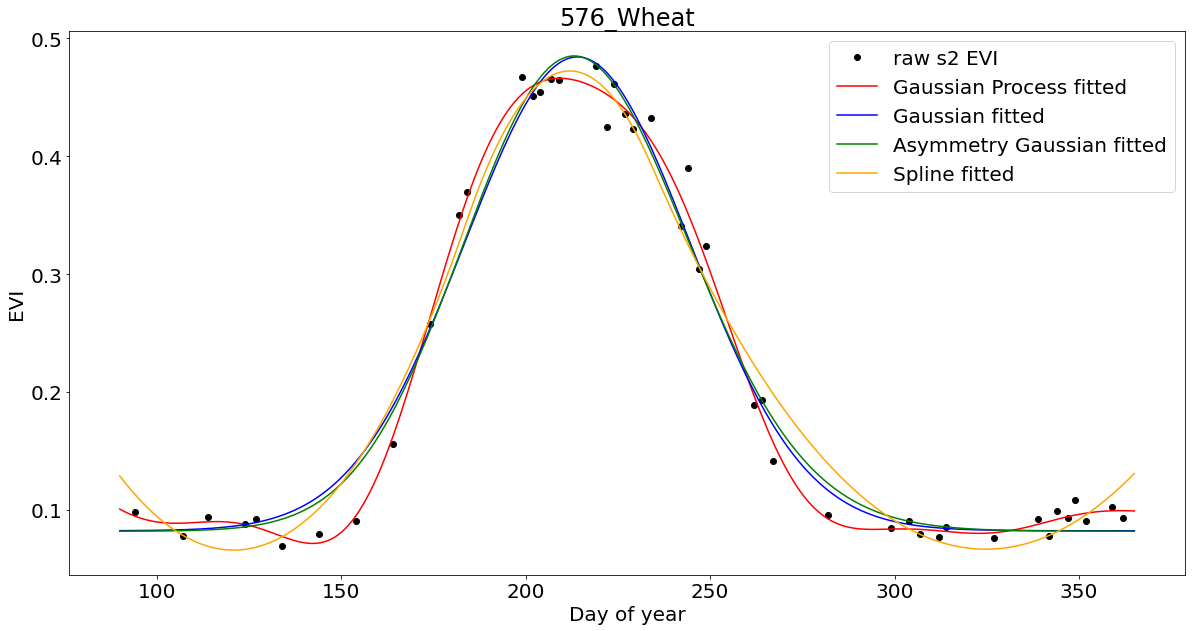
\includegraphics[scale=0.3]{img/yan_wheat_GPR_plot.png}
    \caption{Andries' team found that GPs where superior in terms of predicting a phenological timeline for a number of common seasonal crops over other parameteric models.}
    \label{fig: GP_motivate_wheat}
\end{figure}
Andries' team found that the only draw back to using GPs was the lengthy run time required to create predictions and fears that as more data is collected each season this would only exacerbate the issue. This is a common problem shared by anyone wanting to use GPs. Due to their unwieldy $\calO \left( n^3 \right)$ runtime, where $n$ is the number of observations,  GPs become impractical to apply on datasets with $n > 10^5$. The goal of this thesis is to explore various avenues one can take to replace some of the more intense calculations with computational more efficient approximations without sacrificing a great deal of precision.

Chapter \ref{Chapter1} will give a more mathematical treatment of GPs starting from the ground up by first giving a review of some essential material from functional analysis and then motivating the theory behind GPs before finally ending with a concrete algorithm for GP regression and classification. In chapter FIX and \ref{Chapter3} we shall look at techniques for approximating a large matrix that essentially provides information on how similar each observation is from one other. Chapter \ref{Chapter4} then gives alternative methods for solving linear systems which is an essential component required for GP algorithm to work.

\newpage
\addtocontents{toc}{\protect\setcounter{tocdepth}{2}}
%%%%%%%%%%%%%%%%%%%%%%%%%%%%%%%%%%%%%%%%%%%%%%%%%%%%%%%%%%%%%%%%%%%%%%%%%%%%%%%
\newpage

\section{A Review of Gaussian Processes and Related Topics}\label{Chapter1}
The aim of this chapter is to review some essential mathematical machinery required for us to understand the core concepts of Gaussian Processes.

\subsection{Krylov Subspace Methods}\label{Section1.1}

In this section we will focus on how iterative methods, in particular a class of iterative methods called Krylov Subspace methods, may be used to solve a linear system $\bm{A} \bm{x} = \bm{b}$. While non-iterative methods exist to solve such systems virtually all of them carry an unwieldy runtime of $\mathcal{O} \left( n^3 \right)$ for a system of $n$ parameters. Even for current computer systems, this renders many common matrix problems untractable. Consequently the focus of solving linear systems has shifted towards iterative methods. While iterative methods typically demand certain structural properties of the matrices, such as symmetry and positive definiteness, this generally is not a problem since the majority of large matrix problems that, by mature, endow these systems with the desired properties. For example, in the context of this paper the Gram matrices used to solve linear systems in Gaussian Processes possess both symmetry and positive definiteness. There are also a number of other properties of iterative methods which make them rather attractive to users. To start, iterative Krylov subspace methods are guranteed to converge to an exact solution within a finite number of iterations and even if the method is prematurely stopped before reaching an exact solution, the approximation obtained on the final iteration will in some sense be a good enough estimate of our exact solution. Furthermore, unlike most non-iterative methods, Krylov subspace methods do not require an explicit form of the matrix $\bm{A}$ and instead only requires some routine or process for computing $\bm{A} \bm{x}$.

\subsubsection{Krylov Subspaces}\label{Section1.1.1}

We will motivate the Krylov subspaces by observing their usefullness in solving linear systems. To this end, consider the problem of solving the linear system
\begin{equation}\label{eq: lin_sys_1}
    \bm{A} \bm{x^{\star}} = \bm{b}
\end{equation}
where no explicit form of $\bm{A}$ is available and instead one must draw information from $\bm{A}$ solely through a routine that can evaluate $\bm{A} \bm{v}$ for any $\bm{v}$. How could this routine be utilized in such a manner to provide with a solution to equation \ref{eq: lin_sys_1}? Before answering this, consider the following theorem

\begin{thm} \label{theorem: invert_mat_norm}
    For $\bm{A} \in \KK^{n \times n}$ if $\| \bm{A} \| = q < 1$ then $\Id - \bm{A}$ is invertible and its inverse admits the following representation
    \[
        \left( \Id - \bm{A} \right)^{-1} = \sum_{k=0}^{\infty} \bm{A}^k.
    \]
    \cite{BerezanskyMakarovich1996FaV1}
\end{thm}
Consider a matrix for which $\| \bm{A} \| < 2$, it follows that $\| \Id - \bm{A} \| < 1$ meaning $\Id - \left( \Id - \bm{A} \right)$ is invertible and $\bm{A}^{-1} = \left( \Id - \left( \Id - \bm{A} \right) \right)^{-1} = \sum_{k=0}^{\infty} \left( \Id - \bm{A} \right)^{k}$. Thinking back to equation \ref{eq: lin_sys_1} for any $x_0 \in \KK^{n}$ we have
\begin{align*}
    \bm{x^{\star}} & = \bm{A}^{-1} \bm{b} = \bm{A}^{-1} \left( \bm{A} \bm{x^{\star}} - \bm{A} \bm{x_0} + \bm{A} \bm{x_0} \right) \\
                   & = \bm{x_0} + \bm{A}^{-1} \bm{r_0}                                                                           \\
                   & = \bm{x_0} + \sum_{k=0}^{\infty} \left( \Id - \bm{A} \right)^k
\end{align*}
where $\bm{r_0} = \bm{A} \bm{x^{\star}} - \bm{A} \bm{x_0}$. A natural question that arises is that can we find a closed form solution of the above equation? To answer this question we need to enlist the help of the Cayley-Hamilton theorem.
\begin{thm}[Cayley-Hamilton] \label{theorem: cayley_amilton}
    Let $p_n \left( \lambda \right) = \sum_{i=0}^{n} c_i \lambda^{i}$ be the characteristic polynomial of the matrix $\bm{A} \in \KK^{n \times n}$, then $p_n \left( \bm{A} \right) = \bm{0}$. {\color{red} \textbf{THIS NEEDS A CITATION}}
\end{thm}
The Cayley-Hamilton theorem implies that
\begin{align*}
    0           & = c_0 + c_1 \bm{A} + \ldots + c_{n-1} \bm{A}^{n-1} + c_{n} \bm{A}^{n}           \\
    0           & = \bm{A}^{-1} c_0 + c_1 + \ldots + c_{n-1} \bm{A}^{n-2} + c_{n} \bm{A}^{n-1}    \\
    \bm{A}^{-1} & = \alpha_0 + c_1 + \ldots + \alpha_{n-1} \bm{A}^{n-2} + \alpha_{n} \bm{A}^{n-1}
\end{align*}
where $\alpha_i = -c_i / c_0$. This demonstrates that $\bm{A}^{-1}$ can be represented as a matrix polynomial of degree $n-1$. This means that $\sum_{k=0}^{\infty} \left( \Id - \bm{A} \right)^k$ indeed possess a closed form solution namely
\[
    \bm{x^{\star}} = \bm{x_0} + \bm{A}^{-1} \bm{r_0} = \alpha_0 + c_1 + \ldots + \alpha_{n-1} \bm{A}^{n-2} + \alpha_{n} \bm{A}^{n-1}.
\]
This also shows that $\bm{x^{\star}} \in \operatorname{l.s} \left\{ \bm{r_0}, \bm{A} \bm{r_0}, \bm{A}^2 \bm{r_0}, \ldots , \bm{A}^{n-1} \bm{r_0} \right\}$. One idea for finding a solution to equation \ref{eq: lin_sys_1} is to use our routine for evaluting $\bm{A} \bm{v}$ to iteratively compute new basis elements for the space generated by $\left\{ \bm{r_0}, \bm{A} \bm{r_0}, \bm{A}^2 \bm{r_0}, \ldots , \bm{A}^{n-1} \bm{r_0} \right\}$ and at each step carefully choosing a $\bm{x_k}$ such that $\bm{x_k}$ approaches $\bm{x^{\star}}$, in some form. The subspace constructed using this technique is so important that is has its own name.
\begin{defe}[Krylov Subspace] \label{defe: krylov_subspace}
    The Krylov Subspace of order $k$ generated by the matrix $\bm{A} \in \KK^{n \times n}$ and the vector $\bm{v} \in \KK$ is defined as
    \[
        \calK_{k} \left( \bm{A},\bm{v} \right) = \operatorname{l.s} \left\{ \bm{r_0}, \bm{A} \bm{r_0}, \bm{A}^2 \bm{r_0}, \ldots , \bm{A}^{n-1} \bm{r_0} \right\}
    \]
    for $k \geq 1$ and $\calK_{k} \left( \bm{A},\bm{v} \right) = \left\{ \bm{0} \right\}$.
\end{defe}
For the purposes of solving equation \ref{eq: lin_sys_1} it is of much interest to understand how $\calK_{k} \left( \bm{A},\bm{v} \right)$ grows for larger and larger $k$ since a solution for equation \ref{eq: lin_sys_1} will be present in a Krylov Subspace that cannot be grown any larger. In other words, an exact solution can be constructed once we have extracted all the information from $\bm{A}$ through multiplication of $\bm{r_0}$. The following theorem provides information on how exactly the Krylov Subspace grows as $k$ increases.
\begin{thm} \label{theorem: grade_of_v}
    There is a positive called the grade of $\bm{v}$ with respect to $\bm{A}$, denoted $t_{\bm{v}, \bm{A}}$, where
    \[
        \operatorname{dim} \left( \calK_{k} \left( \bm{A} , \bm{v} \right) \right) = \left\{
        \begin{matrix}
            k, & k \leq t \\
            t, & k \geq t
        \end{matrix}
        \right.
    \]
\end{thm}
Theorem \ref{theorem: grade_of_v} essentially tells us that for $k \leq t_{\bm{v}, \bm{A}}$ that $\bm{A}^k \bm{v}$ is linearly independent to $\bm{A}^i \bm{v}$ for $0 \leq i \leq k-1$ meaning $\left\{ \bm{v}, \bm{A} \bm{v}, \bm{A}^2 \bm{v}, \ldots , \bm{A}^{n-1} \bm{v} \right\}$ serves as a basis for $\calK_{k} \left( \bm{A},\bm{v} \right)$ and that $\calK_{k-1} \left( \bm{A},\bm{v} \right) \subsetneq \calK_{k} \left( \bm{A},\bm{v} \right)$. Conversely, any new vectors formed beyond $t_{\bm{v}, \bm{A}}$ will be linearly independent meaning $\calK_{k} \left( \bm{A},\bm{v} \right) \subsetneq \calK_{k+1} \left( \bm{A},\bm{v} \right)$ for $k \geq t_{\bm{v}, \bm{A}}$. While $t_{\bm{v}, \bm{A}}$ clearly plays a role in determining a suitable basis for which $\bm{A}^{-1} \bm{b}$ lies in its importance is made abundantly clear in the following corollary.
\begin{cor} \label{theorem: grade_as_min}
    \[
        t_{\bm{v}, \bm{A}} = \min \left\{k \mid \bm{A}^{-1} \bm{v} \in \calK_{k} \left( \bm{A},\bm{v} \right) \right\}
    \]
\end{cor}
\begin{proof}
    Recall from Cayley-Hamilton (theorem \ref{theorem: cayley_amilton}) that
    \[
        \bm{A}^{-1} \bm{v} = \sum_{i=0}^{n-1} \alpha_{i} \bm{A}^{i} \bm{v}
    \]
    But since $\calK_{k} \left( \bm{A},\bm{v} \right) = \calK_{k+1} \left( \bm{A},\bm{v} \right)$ for $k \geq t_{\bm{v}, \bm{A}}$
    \[
        \bm{A}^{-1} \bm{v} = \sum_{i=0}^{t-1} \beta_{i} \bm{A}^{i} \bm{v}
    \]
    meaing $\bm{A}^{-1} \bm{v} \in \calK_{k} \left( \bm{A},\bm{v} \right)$ for $k \geq t_{\bm{v}, \bm{A}}$. Suppose for the sake of contradiction that this also holds for $k = t_{\bm{v}, \bm{A}} - 1$, that is, $\bm{A}^{-1} \bm{v} = \sum_{i=0}^{t-2} \gamma_{i} \bm{A}^{i} \bm{v}$. However, this gives
    \[
        \bm{v} = \sum_{i=0}^{t-2} \gamma_{i} \bm{A}^{i+1} \bm{v} = \sum_{i=0}^{t-1} \gamma_{i-1} \bm{A}^{i} \bm{v}
    \]
    implying $\left\{ \bm{v}, \bm{A} \bm{v}, \bm{A}^2 \bm{v}, \ldots , \bm{A}^{t-1} \bm{v} \right\}$ are linearly dependent which means that $\operatorname{dim} \left( \calK_{k} \left( \bm{A} , \bm{v} \right) \right) < t$, which provides us with our contrdiction.
\end{proof}
This machinery allows us to make a much stronger statement on the where abouts of $\bm{x^{\star}}$ in relation to the Krylov Subspaces.
\begin{cor} \label{theorem: sol_in_krylov}
    For any $\bm{x_0}$, we have
    \[
        \bm{x^{\star}} \in \bm{x_0} + \calK_{t_{\bm{r_0}, \bm{A}}} \left( \bm{A},\bm{r_0} \right)
    \]
    where $\bm{r_0} = \bm{b} - \bm{A} \bm{x_0}$.
\end{cor}

\subsubsection{Gram-Schmidt Process and QR factorisations}\label{Section1.1.2}

Many areas of linear algebra involving studing the column space of matrices. The $QR$ factorisation provides us with a powerful tool to better understand the column space of a matrix as well as serving as an important factorisation mechanism for many numerical methods. Suppose that a matrix $\bm{A} = \left[ \bm{a}_1 , \bm{a}_2 , \ldots , \bm{a}_n \right] \in \KK^{n \times n}$ has full rank. The idea of a $QR$ factorisation is to find an alternative orthornormal basis for $\left( \bm{a}_i \right)_{i=1}^{n}$, say $\left( \bm{q}_i \right)_{i=1}^{n}$, and to somehow relate the original matrix $\bm{A}$ to a new matrix whose columns are $\left( \bm{q}_i \right)_{i=1}^{n}$. Consider the following procedure that allows us to find an orthornormal basis $\left( \bm{q}_i \right)_{i=1}^{n}$ for which $\operatorname{l.s} \left\{ \left( \bm{a}_i \right)_{i=1}^{n} \right\} = \operatorname{l.s} \left\{ \left( \bm{q}_i \right)_{i=1}^{n} \right\}$. First set $\bm{q}_1 = \frac{\bm{a}_1}{\| \bm{a}_i \|}$, clearly $\operatorname{l.s} \left\{ \bm{a}_1 \right\} = \operatorname{l.s} \left\{ \bm{q}_1 \right\}$. Next, construct a vector $\bm{q}_2' = \bm{a}_2 - r_{1,2} \cdot \bm{q}_1$ so that $\bm{q}_2' \perp \bm{q}_1$. This means
\begin{align*}
    0       & = \langle \bm{q}_1, \bm{q}_2' \rangle                                                   \\
    0       & = \langle \bm{q}_1, \bm{a}_2 - r_{1,2} \cdot \bm{q}_1 \rangle                           \\
    0       & = \langle \bm{q}_1, \bm{a}_2 \rangle - r_{1,2} \cdot \langle \bm{q}_1, \bm{q}_1 \rangle \\
    r_{1,2} & = \langle \bm{q}_1, \bm{a}_2 \rangle
\end{align*}
Since $\bm{q}_2'$ may not be a unit vector we set $\bm{q}_2 = \frac{\bm{q}_2'}{\| \bm{q}_2' \|}$ where $\operatorname{l.s} \left( \left\{ \bm{a}_1, \bm{a}_2 \right\} \right) = \operatorname{l.s} \left( \left\{ \bm{q}_1, \bm{q}_2 \right\} \right)$. Continuing the vector $\bm{q}_3'$ is constructed so that
\[
    \bm{q}_3' = \bm{a}_3 - \bm{r}_{1,3} \bm{q}_1 - \bm{r}_{2,3} \bm{q}_2
\]
are chosen so that $\bm{q}_3'$ is orthogonal to both $\bm{q}_2$ and $\bm{q}_1$. This amounts to setting $r_{1,3} = \langle \bm{q}_1, \bm{a}_3 \rangle$ and $r_{2,3} = \langle \bm{q}_2, \bm{a}_{3} \rangle$. Similarly, $\bm{q}_3'$ is normalized so that $\bm{q}_3 = \frac{\bm{q}_3'}{\| \bm{q}_3' \|}$ and $\operatorname{l.s} \left( \left\{ \bm{a}_1, \bm{a}_2, \bm{a}_3 \right\} \right) = \operatorname{l.s} \left( \left\{ \bm{q}_1, \bm{q}_2, \bm{q}_3 \right\} \right)$. Continuing in this fashion the $k^{th}$ vector in our orthornormal basis is computed as
\begin{equation}\label{eq: comp_orth_basis}
    \bm{q}_k = \frac{\bm{a}_k - \sum_{i=1}^{k-1} r_{i,k} \cdot \bm{q}_i}{r_{k,k}}
\end{equation}
where $r_{i,k} = \langle \bm{q}_i, \bm{a}_k \rangle$, $r_{k,k} = \| \bm{a}_k - \sum_{i=1}^{k-1} r_{i,k} \cdot \bm{q}_i \|$ and $\operatorname{l.s} \left( \left\{ \bm{a}_1, \bm{a}_2, \ldots , \bm{a}_k \right\} \right) = \operatorname{l.s} \left( \left\{ \bm{q}_1, \bm{q}_2, \ldots , \bm{q}_k \right\} \right)$. This procedure is famiously known as the Gram-Schmidt process \cite{BerezanskyMakarovich1996FaV1,TrefethenLloydN.LloydNicholas1997Nla/,DemmelJamesW1997Anla} and is summarized in the following algorithm.

    % https://tex.stackexchange.com/questions/463359/algorithm-inside-a-tcolorbox-how-to-put-a-label-to-the-algorithm-but-the-captio
    % http://cfrgtkky.blogspot.com/2018/12/algorithm-inside-tcolorbox-how-to-put.html
    % {\centering
    %     \begin{minipage}{.85\linewidth}
    %         \begin{tcolorbox}[colback=white!100,colframe=black!100]
    %             \begin{algorithm}[H]
    %                 \caption{Classical Gram-Schmidt}
    % \label{alg: Classical_Gram-Schmidt}
    % \SetAlgoLined
    % \DontPrintSemicolon
    % \SetKwInOut{Input}{input}\SetKwInOut{Output}{output}

    % \Input{A basis $\left( \bm{a}_i \right)_{i=1}^{n}$.}
    % \Output{An orthornormal basis $\left( \bm{q}_i \right)_{i=1}^{n}$ such that $\operatorname{l.s} \left\{ \left( \bm{a}_i \right)_{i=1}^{n} \right\} = \operatorname{l.s} \left\{ \left( \bm{q}_i \right)_{i=1}^{n} \right\}$}
    % \BlankLine
    % \For{$k = 1$ \KwTo $n$}{
    %     $\bm{q}_k' = \bm{a}_k$\;
    %     \For{$i = 1$ \KwTo $k-1$}{
    %         $r_{i,k} = \langle \bm{q}_i, \bm{a}_k \rangle$\;
    %         $\bm{q}_k' = \bm{q}_k' - r_{i,k} \bm{q}_i$\;
    %     }
    %     $r_{k,k} = \| \bm{q}_k' \|$\;
    %     $\bm{q}_k = \bm{q}_k' / r_{k,k}$\;
    % }
    % \Return{$\left( \bm{q}_i \right)_{i=1}^{n}$}
    % \BlankLine
    %             \end{algorithm}
    %         \end{tcolorbox}
    %     \end{minipage}
    %     \par
    % }


    {\centering
        \begin{minipage}{.85\linewidth}
            \begin{algorithm}[H]
                \caption{Classical Gram-Schmidt}
                \label{alg: Classical_Gram-Schmidt}
                \SetAlgoLined
                \DontPrintSemicolon
                \SetKwInOut{Input}{input}\SetKwInOut{Output}{output}

                \Input{A basis $\left( \bm{a}_i \right)_{i=1}^{n}$.}
                \Output{An orthornormal basis $\left( \bm{q}_i \right)_{i=1}^{n}$ such that $\operatorname{l.s} \left\{ \left( \bm{a}_i \right)_{i=1}^{n} \right\} = \operatorname{l.s} \left\{ \left( \bm{q}_i \right)_{i=1}^{n} \right\}$}
                \BlankLine
                \For{$k = 1$ \KwTo $n$}{
                    $\bm{q}_k' = \bm{a}_k$\;
                    \For{$i = 1$ \KwTo $k-1$}{
                        $r_{i,k} = \langle \bm{q}_i, \bm{a}_k \rangle$\;
                        $\bm{q}_k' = \bm{q}_k' - r_{i,k} \bm{q}_i$\;
                    }
                    $r_{k,k} = \| \bm{q}_k' \|$\;
                    $\bm{q}_k = \bm{q}_k' / r_{k,k}$\;
                }
                \Return{$\left( \bm{q}_i \right)_{i=1}^{n}$}
                \BlankLine
            \end{algorithm}
        \end{minipage}
        \par
    }

Relating the column space of $\bm{A}$ to the orthornormal basis $\left( \bm{q}_{i} \right)_{i=1}^{n}$ in a matrix form
\[
    \left[ \bm{a}_1 , \bm{a}_2 , \ldots \bm{a}_n \right] =
    \left[ \bm{q}_1 , \bm{q}_2 , \ldots \bm{q}_n \right]
    \begin{bmatrix}
        r_{1,1} & r_{1,2} & \cdots & r_{1,n} \\
                & r_{2,2} &        & \vdots  \\
                &         & \ddots & \vdots  \\
                &         &        & r_{n,n}
    \end{bmatrix}
\]
or more succinctly
\begin{equation}\label{eq: QR_factorisation}
    \bm{A} = \bm{Q} \bm{R}
\end{equation}
where $\bm{Q} = \left[ \bm{q}_1 , \bm{q}_2 , \ldots \bm{q}_n \right]$ and $\left( \bm{R} \right)_{i,j} = r_{i,j}$ for $i \leq j$ and $\left( \bm{R} \right)_{i,j} = 0$ for $i > j$. This is exactly the $QR$ factorisation for a full rank matrix. Note that $\operatorname{Range} \left( \bm{A} \right) = \operatorname{Range} \left( \bm{Q} \right)$. In general, any square matrix  $\bm{A} \in \KK^{m \times n}$ may be decomposed as $\bm{A} = \bm{Q} \bm{R}$ where $\bm{Q} \in \KK^{m \times m}$ is an orthogonal matrix and $\bm{R} \in \KK^{m \times n}$ is an upper triangular matrix. This is known as a full $QR$ factorisation. Since bottom $(m-n)$ rows of this $\bm{R}$ consists entirely of zeros, it is often useful to partition the full $QR$ factorisation in the following manner to shed vacuous entries
\[
    \bm{A} = \bm{Q} \bm{R} = \bm{Q}
    \begin{bmatrix}
        \hat{\bm{R}} \\
        \bm{0}_{(m-n) \times n}
    \end{bmatrix}
    =
    \begin{bmatrix}
        \hat{\bm{Q}} & \bm{Q}'
    \end{bmatrix}
    \begin{bmatrix}
        \hat{\bm{R}} \\
        \bm{0}_{(m-n) \times n}
    \end{bmatrix}
    = \hat{\bm{Q}} \hat{\bm{R}}.
\]
This alternate decomposition is called the reduced (or somtimes the thin) QR-factorization. We shall state the following two theorems on the QR-factorization are stated without proof.

\begin{thm} \label{theorem: QR_general_existence}
    Every $\bm{A} \in \KK^{m \times n}, \; (m \geq n)$ has a full $QR$ factorisation, hence also a reduced $QR$ factorisation.
    \cite{TrefethenLloydN.LloydNicholas1997Nla/}
\end{thm}

\begin{thm} \label{theorem: QR_full_rank_unique}
    Each $\bm{A} \in \KK^{m \times n}, \; (m \geq n)$ of full rank has a unique reduced $QR$ factorisation $\bm{A} = \hat{\bm{Q}} \hat{\bm{R}}$ with $r_{k,k} > 0$.
    \cite{TrefethenLloydN.LloydNicholas1997Nla/}
\end{thm}

In practice the classical Gram-Schmidt process described in algorithm \ref{alg: Classical_Gram-Schmidt} is rarely used as the procedure becomes numerically unstable if $\left( \bm{a}_i \right)_{i=1}^{n}$ are almost linearly dependent. Before looking for ways to resolve these numerical instabilities a quick recap of projectors has been devised. A square matrix $\bm{P}_{G}$ acting on a Hilbert space $H$ that sends $\bm{x} \in H$ to its projection onto a subspace $G$ is called the projector onto $G$. If $\left( \bm{q}_k \right)_{k=1}^{m}$ is an orthornormal basis in $G$ then
\[
    \bm{P}_{G} = \bm{Q} \bm{Q}^{\ast}
\]
where $\bm{Q} = \left[ \bm{q}_1 , \bm{q}_2 , \ldots \bm{q}_m, 0 , \ldots , 0 \right] \in \KK^{n \times n}$. A special class of projectors which isolates the components of a given vector onto a one dimensional subspace spanned by a single unit vector $\bm{q}$ called a rank one orthogonal projector, denoted as $\bm{P}_{q}$. Each $k$ in the classical Gram-Schmidt process $\bm{q}_k'$ using the following orthogonal projection
\begin{equation}\label{eq: classical_GS_proj}
    \bm{q}_k' = \bm{P}_{A_{k}^{\perp}} \bm{a}_k
\end{equation}
where $A_k = \operatorname{l.s} \left\{ \bm{a}_i \right\}_{i=1}^{k}$ and $\bm{P}_{A_{1}^{\perp}} = \Id$ for convenience. A modified version of the Gram-Schmidt process performs the same orthogonal projection broken up as $k-1$ orthogonal projections of rank $n-1$ as so
\begin{align*}
    \bm{q}_k' & = \bm{P}_{A_{k}^{\perp}} \bm{a}_k                                                                                                                                   \\
              & = \left( \Id - \bm{Q}_{k} \bm{Q}_{k}^{\ast} \right) \bm{a}_k                                                                                                        \\
              & = \left( \prod_{i=1}^{k-1} \left( \Id - \bm{q}_i \bm{q}_i^{\ast} \right) \right)\bm{a}_k                                                                            \\
              & = \left( \Id - \bm{q}_1 \bm{q}_1^{\ast} \right) \left( \Id - \bm{q}_1 \bm{q}_1^{\ast} \right) \cdots \left( \Id - \bm{q}_{k-1} \bm{q}_{k-1}^{\ast} \right) \bm{a}_k \\
              & = \bm{P}_{\bm{q}_{k}^{\perp}} \cdots \bm{P}_{\bm{q}_{1}^{\perp}} \bm{a}_k
\end{align*}

While its clear that $\bm{P}_{A_{k}^{\perp}} \bm{a} $ and $\bm{P}_{\bm{q}_{k}^{\perp}} \cdots \bm{P}_{\bm{q}_{1}^{\perp}} \bm{a}_k$ used for computing $\bm{q}_k'$ are algebraically, they differ arithmetically as the latter expression evaluates $\bm{q}_k'$ using the follow procedure

\begin{align*}
    \bm{q}_k^{(1)}             & = \bm{a}_k                                       \\
    \bm{q}_k^{(2)}             & = \bm{P}_{\bm{q}_{1}^{\perp}} \bm{q}_k^{(1)}     \\
    \bm{q}_k^{(3)}             & = \bm{P}_{\bm{q}_{2}^{\perp}} \bm{q}_k^{(2)}     \\
                               & \vdots                                           \\
    \bm{q}_k' = \bm{q}_k^{(k)} & = \bm{P}_{\bm{q}_{k-1}^{\perp}} \bm{q}_k^{(k-1)}
\end{align*}

Applying projections sequentially in this manner produces smaller numerical errors. The modified Gram-Schmidt process \cite{TrefethenLloydN.LloydNicholas1997Nla/,DemmelJamesW1997Anla} is summarized in the following algorithm.

    {\centering
        \begin{minipage}{.85\linewidth}
            \begin{algorithm}[H]
                \caption{Modified Gram-Schmidt}
                \label{alg: Modified_Gram-Schmidt}
                \SetAlgoLined
                \DontPrintSemicolon
                \SetKwInOut{Input}{input}\SetKwInOut{Output}{output}

                \Input{A basis $\left\{ \bm{a}_i \right\}_{i=1}^{n}$.}
                \Output{An orthornormal basis $\left\{ \bm{q}_i \right\}_{i=1}^{n}$ such that $\operatorname{l.s} \left\{ \bm{a}_i \right\}_{i=1}^{n} = \operatorname{l.s} \left\{  \bm{q}_i \right\}_{i=1}^{n}$}
                \BlankLine
                \For{$k = 1$ \KwTo $n$}{
                    $\bm{q}_k' = \bm{a}_k$\;
                }
                \For{$k = 1$ \KwTo $n$}{
                    $r_{k,k} = \| \bm{q}_k' \|$\;
                    $\bm{q}_k = \bm{q}_k' / r_{k,k}$\;
                    \For{$i = k+1$ \KwTo $n$}{
                        $r_{i,k} = \langle \bm{q}_k, \bm{q}_i' \rangle$\;
                        $\bm{q}_i = \bm{q}_i - r_{i,k} \bm{q}_i$\;
                    }
                }
                \Return{$\left\{ \bm{q}_i \right\}_{i=1}^{n}$}
                \BlankLine
            \end{algorithm}
        \end{minipage}
        \par
    }

\subsubsection{Arnoldi and Lanczos Algorithm}\label{Section1.1.3}

As a quick reminder, we are in search of an iterative process to solve the linear system $\bm{A} \bm{x}^{\star} = \bm{b}$ where no explicit form of $\bm{A}$ is available and we may only rely on a routine that computes $\bm{A} \bm{v}$ for any $\bm{v}$ to extract information on $\bm{A}$. In section \ref{Section1.1.1} we discovered that $\bm{x}^{\star} \in \calK_{t_{\bm{r}_0}, \bm{A}} \left( \bm{A}, \bm{r}_0 \right)$. With many iterative methods, computing an exact value for $\bm{x}^{\star}$ is out the question with the view that $t_{\bm{r}_0, \bm{A}}$ is impractically large. We must instead resort to approximating $\bm{x}^{\star}$ by $\bm{x}_k$ for which $\bm{x}^{k} \in \calK_{k} \left( \bm{A}, \bm{r}_0 \right)$ where $k \ll t_{\bm{r}_0}$. To find an appropriate value for $\bm{x}_k$, a good start would be to find a basis $\calK_{k} \left( \bm{A}, \bm{r}_0 \right)$. Definition \ref{defe: krylov_subspace} showed us that $\left\{ \bm{A}^{i-1} \bm{r}_0 \right\}_{i=1}^{k}$ serves as a basis for $\calK_{k} \left( \bm{A}, \bm{r}_0 \right)$. However, for numericcal reasons this is a poor choice of basis since this each consecutive term becomes closer and closer to being linearly dependent. To search for a more appriporate basis, set $n = t_{\bm{r}_0, \bm{A}}$ so that $\bm{x}^{\star} \in \calK_{n} \left( \bm{A}, \bm{r}_0 \right)$. Let $\bm{K} \in \KK^{n \times n}$ be the invertible matrix
\[
    \bm{K} = \left[ \bm{r}_0 , \bm{A} \bm{r}_0, \ldots , \bm{A}^{n-1} \bm{r}_0 \right].
\]
Since $\bm{K}$ is invertible we can compute $\bm{c} = - \bm{K}^{-1} \bm{A}^{n} \bm{r}_0$ so that
\begin{align*}
    \bm{A} \bm{K} & = \left[ \bm{A} \bm{r}_0, \bm{A}^{2} \bm{r}_0, \ldots , \bm{A}^{n} \bm{r}_0 \right]                     \\
    \bm{A} \bm{K} & = \bm{K} \cdot \left[ \bm{e}_2, \bm{e}_3, \ldots , \bm{e}_n, - \bm{c}  \right] \triangleq \bm{K} \bm{C}
\end{align*}
or, in a more verbose form
\[
    \bm{K}^{-1} \bm{A} \bm{K} = \bm{C} =
    \begin{bmatrix}
        0      & 0      & \cdots & 0      & -c_1   \\
        1      & 0      & \cdots & 0      & -c_2   \\
        0      & 1      & \cdots & 0      & \vdots \\
        \vdots & \vdots & \cdots & \vdots & \vdots \\
        0      & 0      & \cdots & 1      & -c_n
    \end{bmatrix}.
\]
Note here that $\bm{C}$ is upper Hessenberg. While this form is simple, it is of little practical use since the matrix $\bm{K}$ is very likely to be ill-conditioned. To remedy this we can replace $\bm{K}$ with an orthogonal matrix which spans the same space. These are exactly the properties that the $\bm{Q}$ matrix offers in the $QR$-factorisation of $\bm{K}$. With this in mind let $\bm{K} = \bm{Q} \bm{R}$ be the full $QR$-factorisation of $\bm{K}$. Then
\begin{align*}
    \bm{A} \bm{Q} \bm{R} & = \bm{A} \bm{K}                    \\
    \bm{A} \bm{Q}        & = \bm{A} \bm{K} \bm{R}^{-1}        \\
    \bm{A} \bm{Q}        & = \bm{K} \bm{C} \bm{R}^{-1}        \\
    \bm{A} \bm{Q}        & = \bm{Q} \bm{R} \bm{C} \bm{R}^{-1} \\
    \bm{A} \bm{Q}        & \triangleq \bm{Q} \bm{H}.
\end{align*}
Since $\bm{R}$ and $\bm{R}^{-1}$ and both upper triangular and $\bm{C}$ is upper Hessenberg, $\bm{H}$ is also upper Hessenberg. This form provides us with a $\bm{Q}$ such that the range of $\bm{Q}$ is $\calK_{n} \left( \bm{A}, \bm{r}_0 \right)$ and
\begin{equation}\label{eq: QTAQ_eq_H}
    \bm{Q}^{\intercal} \bm{A} \bm{Q} = \bm{H}.
\end{equation}
Again, in practice, it may be very difficult to compute this entire expression forcing us to search for approximative alternatives. Consider equation \ref{eq: QTAQ_eq_H} for which the only first $k$ columns of $\bm{Q}$ have been computed. Let $\bm{Q}_k = \left[ \bm{q}_1 , \bm{q}_2 , \ldots , \bm{q}_k \right]$ and $\bm{Q}_u = \left[ \bm{q}_{k+1} , \bm{q}_{k+2} , \ldots , \bm{q}_{n} \right]$. Then
\begin{align*}
    \bm{Q}^{\intercal} \bm{A} \bm{Q}                                                         & = \bm{H} \\
    \left[ \bm{Q}_k , \bm{Q}_u \right]^{\intercal} \bm{A} \left[ \bm{Q}_k , \bm{Q}_u \right] & =
    \begin{bmatrix}
        \bm{H}_k     & \bm{H}_{u,k} \\
        \bm{H}_{k,u} & \bm{H}_{u}
    \end{bmatrix}                                                                           \\
    \begin{bmatrix}
        \bm{Q}_{k}^{\intercal} \bm{A} \bm{Q}_{k} & \bm{Q}_{k}^{\intercal} \bm{A} \bm{Q}_{u} \\
        \bm{Q}_{u}^{\intercal} \bm{A} \bm{Q}_{k} & \bm{Q}_{u}^{\intercal} \bm{A} \bm{Q}_{u}
    \end{bmatrix}
                                                                                             & =
    \begin{bmatrix}
        \bm{H}_k     & \bm{H}_{u,k} \\
        \bm{H}_{k,u} & \bm{H}_{u}
    \end{bmatrix}
\end{align*}
where $\bm{H}_k , \bm{H}_{u,k}, \bm{H}_{k,u}$ and $\bm{H}_u$ are the relevant sub matrices. This provides us with the equality
\begin{equation}\label{eq: QTkAQk_eq_Hk}
    \bm{Q}_{k}^{\intercal} \bm{A} \bm{Q}_{k} = \bm{H}_k
\end{equation}
noting that $\bm{H}_{k}$ is upper Hessenberg for the same reason that $\bm{H}$ is. We know that when $n = t_{\bm{r}_0, \bm{A}}$ we can find a $\bm{Q} \in \KK^{n \times n}$ and $\bm{H} \in \KK^{n \times n}$ that satisfies $\bm{A} \bm{Q} = \bm{Q} \bm{H}$. However, in general, we may not be so fortunate in finding a $\bm{Q}_{k} \in \KK^{n \times k}$ and $\bm{H}_{k} \in \KK^{n \times k}$ so satisfy $\bm{A} \bm{Q}_{k} = \bm{Q}_{k} \bm{H}_k$ for any $k < n$. Instead we can adjust this equality by adding an error $\bm{E}_k \in \KK^{n \times k}$ so that we do get equality. Our expression now becomes
\begin{equation}\label{eq: QTkAQk_eq_HkEk}
    \bm{Q}_{k}^{\intercal} \bm{A} \bm{Q}_{k} = \bm{H}_k + \bm{E}_k.
\end{equation}
A careful choice of $\bm{E}_k$ must be made to also retain equality in equation \ref{eq: QTkAQk_eq_Hk}, meaning $\bm{Q}_{k}^{\intercal} \bm{E}_k = \bm{0}$. Since $\left\{ \bm{q}_i \right\}_{i=1}^{k}$ forms an orthornormal basis for $\calK_{n} \left( \bm{A}, \bm{r}_0 \right)$, consider the following choice of $\bm{E}_k$,
\[
    \bm{E}_k = \bm{q}_{k+1} \bm{h}_{k}^{\intercal}
\]
where $\bm{h}_k$ is any vector in $\KK^{k}$. Notice that
\[
    \bm{Q}_{k}^{\intercal} \bm{E} = \bm{Q}^{\intercal} \left( \bm{q}_{k+1} \bm{h}_k \right) = \left( \bm{Q}^{\intercal} \bm{q}_{k+1} \right) \bm{h}_{k}^{\intercal} = \bm{0}.
\]
Since this holds for any $\bm{h}_k \in \KK^{k}$, to preserve sparsity and to keep this form as simple as possible we can set $\bm{h}_k = \left[ 0,0, \ldots , h_{k+1,k} \right]^{\intercal}$. This means $\bm{A} \bm{Q}_k$ can be written as
\begin{equation}\label{eq: QTkAQk_eq_Hk_p_qkhk}
    \bm{A} \bm{Q}_k =  \bm{Q}_k \bm{H}_k + \bm{q}_{k+1} \bm{h}_{k}^{\intercal}
\end{equation}
where
\[
    \bm{Q}_k \bm{H}_k =
    \left[ \bm{q}_1 , \bm{q}_2 , \ldots , \bm{q}_k \right]
    \begin{bmatrix}
        h_{1,1} & \cdots & \cdots & \cdots    & h_{1,k}   \\
        h_{2,1} & \cdots & \cdots & \cdots    & \vdots    \\
        0       & \ddots & \ddots & \ddots    & \vdots    \\
        \vdots  & \ddots & \ddots & \ddots    & \vdots    \\
        0       & \cdots & 0      & h_{k,k-1} & h_{k,k}   \\
        0       & \cdots & 0      & 0         & h_{k+1,k}
    \end{bmatrix}.
\]
Equating the $j^{th}$ columns of equation \ref{eq: QTkAQk_eq_Hk_p_qkhk} yields
\[
    \bm{A} \bm{q}_j = \sum_{i=1}^{j+1} h_{i,j} \bm{q}_{i}.
\]
Again since $\left\{ \bm{q}_i \right\}_{i=1}^{n}$ form an orthornormal basis, multiplying both sides by $\bm{q}_m$ for $1 \leq m \leq j$ gives
\[
    \bm{q}_m^{\intercal} \bm{A} \bm{q}_j = \sum_{i=1}^{j+1} h_{i,j} \bm{q}_m^{\intercal} \bm{q}_{i} = h_{m,j}
\]
and so
\begin{equation}\label{eq: arn_eq_1}
    h_{j+1,j} \bm{q}_{j+1} = \bm{A} \bm{q}_j - \sum_{i=1}^{j} h_{i,j} \bm{q}_{i}.
\end{equation}
From equation \ref{eq: arn_eq_1} we find that $\bm{q}_{j+1}$ can be computed using a recurrance involving its previous Krylov factors. Notice this bears a striking resemblance to equation \ref{eq: comp_orth_basis} having a virtually an identical setup to computing an orthornormal basis using the modified Gram-Schmidt process (algorithm \ref{alg: Modified_Gram-Schmidt}). As such, values for $\bm{q}_{j+1}$ and $h_{j+1,j}$ can be evaluted using a procedure very similar to the modified Gram-Schmidt process better known as the Arnoldi algorithm \cite{TrefethenLloydN.LloydNicholas1997Nla/,DemmelJamesW1997Anla}, presented in algorithm \ref{alg: Arnoldi_Algorithm}.

{\centering
\begin{minipage}{.85\linewidth}
    \begin{algorithm}[H]
        \caption{Arnoldi Algorithm}
        \label{alg: Arnoldi_Algorithm}
        \SetAlgoLined
        \DontPrintSemicolon
        \SetKwInOut{Input}{input}\SetKwInOut{Output}{output}

        \Input{$\bm{A}, \bm{r}_0$ and $k$, the number of columns of $\bm{Q}$ to compute.}
        \Output{$\bm{Q}_k , \bm{H}_k$.}
        \BlankLine
        $\bm{q}_1 = \bm{r}_0 / \| \bm{r}_0 \|$\;
        \For{$j = 1$ \KwTo $k$}{
            $\bm{z} = \bm{A} \bm{q}_j$\;
            \For{$i = 1$ \KwTo $j$}{
                $h_{i,j} = \langle \bm{q}_{i} , \bm{z} \rangle$\;
                $\bm{z} = \bm{z} - h_{i,j} \bm{q}_{i}$\;
            }
            $h_{j+1,j} = \| \bm{z} \|$\;
            \If{$h_{j+1,j} = 0$}{
                \Return{$\bm{Q}_k , \bm{H}_k$}
            }
            $\bm{q}_{j+1} = \bm{z} / h_{j+1,j}$\;
        }
        \Return{$\bm{Q}_k , \bm{H}_k$}
        \BlankLine
    \end{algorithm}
\end{minipage}
\par
}

When $\bm{A}$ is symmertic then $\bm{H} = \bm{T}$ becomes a tridiagonal matrix, simplifying a large amount of the Arnoldi algorithm since a considerably large number of matrix elements from $\bm{T}$ can be written as
\[
    \bm{T} =
    \begin{bmatrix}
        \alpha_1 & \beta_1 &        &             &             \\
        \beta_1  & \ddots  & \ddots &             &             \\
                 & \ddots  & \ddots & \ddots      &             \\
                 &         & \ddots & \ddots      & \beta_{n-1} \\
                 &         &        & \beta_{n-1} & \alpha_{n}
    \end{bmatrix}.
\]
As before, equating the $j^{th}$ columns of $\bm{A} \bm{Q} = \bm{Q} \bm{T}$ yields
\begin{equation}\label{eq: lancz_orth_basis}
    \bm{A} \bm{q}_{j} = \beta_{j-1} \bm{q}_{j-1} + \alpha_{j} \bm{q}_j + \beta_j \bm{q}_{j+1}.
\end{equation}
Again since $\left\{ \bm{q}_{i} \right\}_{i=1}^{n}$ form an orthornormal basis, multiplying both sides of equation \ref{eq: lancz_orth_basis} by $\bm{q}_j$ gives $\bm{q}_j = \bm{A} \bm{q}_j = \alpha_j$. A simplified version of the Arnoldi algorithm can be devised can be used to compute $\left\{ \bm{q}_{i} \right\}_{i=1}^{n}$ and $\bm{T}$ for symmetric matrices known as the Lanczos algorithm \cite{DemmelJamesW1997Anla}. The Lanczos algorithm is presented in algorithm \ref{alg: Lanczos_Algorithm}.

{\centering
\begin{minipage}{.85\linewidth}
    \begin{algorithm}[H]
        \caption{Lanczos Algorithm}
        \label{alg: Lanczos_Algorithm}
        \SetAlgoLined
        \DontPrintSemicolon
        \SetKwInOut{Input}{input}\SetKwInOut{Output}{output}

        \Input{$\bm{A}, \bm{r}_0$ and $k$, the number of columns of $\bm{Q}$ to compute.}
        \Output{$\bm{Q}_k , \bm{T}_k$.}
        \BlankLine
        $\bm{q}_1 = \bm{r}_0 / \| \bm{r}_0 \|$, $\beta_0 = 0$, $\bm{q}_0 = 0$\;
        \For{$j = 1$ \KwTo $k$}{
            $\bm{z} = \bm{A} \bm{q}_j$\;
            $\alpha_j = \langle \bm{q}_{j}, \bm{z} \rangle$\;
            $\bm{z} = \bm{z} - \alpha_j \bm{q}_{j} - \beta_{j-1} \bm{q}_{j-1}$\;
            $\beta_j = \| z \|$\;
            \If{$\beta_{j} = 0$}{
                \Return{$\bm{Q}_k , \bm{T}_k$}
            }
            $\bm{q}_{j+1} = \bm{z} / \beta_{j}$\;
        }
        \Return{$\bm{Q}_k , \bm{T}_k$}
        \BlankLine
    \end{algorithm}
\end{minipage}
\par
}

\subsubsection{Optimality Conditions}\label{Section1.1.4}

So far we have shown that $\bm{x}^{\star} \in \calK_{t_{\bm{r}_0}, \bm{A}} \left( \bm{A}, \bm{r}_0 \right)$ where $n = t_{\bm{r}_0}$ is the grade of $\bm{r}_0$ with respect to $\bm{A}$. Moreover from section \ref{Section1.1.3} we found ways to construct a basis for $\calK_{t_{\bm{r}_0}, \bm{A}} \left( \bm{A}, \bm{r}_0 \right)$ allowing us to generate vectors with these affine spaces, namely the Arnoldi algorithm (algorithm \ref{alg: Arnoldi_Algorithm})and Lanczos algorithm (algorithm \ref{alg: Lanczos_Algorithm}) for non-symmertic and symmertic systems respectively. From now on $\calK_{t_{\bm{r}_0}, \bm{A}} \left( \bm{A}, \bm{r}_0 \right)$ will be abbreviated to $\calK_{t_{\bm{r}_0}, \bm{A}}$ when the context is clear. The question still remains however, how should one choose an $\bm{x}_k$ that best approximates $\bm{x}^{\ast}$ satisfying equation \ref{eq: lin_sys_1}? Here are a few of the most well known methods for selecting a suitable $\bm{x}_k$.

\begin{enumerate}

    \item Select an $\bm{x}_k \in \bm{x}_0 + \calK_k$ which minimizes $\| \bm{x}_k - \bm{x}^{\ast} \|_2$. While this method seems like the most intuitive and natural way to select $\bm{x}_k$, it is unfortunately of no practical use since there is not enough information in the Krylov subspace to find an $\bm{x}_k$ which matches this specification.

    \item Select an $\bm{x}_k \in \bm{x}_0 + \calK_k$ which minimizes $\| \bm{r}_k \|_2$ (recall is the residual of $\bm{x}_k$, that is, $\bm{r}_k = \bm{b} - \bm{A} \bm{x}_k$). This method is possible to implement. Two well known algorithms stem from this class of methods, notably MINRES (minimum residual) and GMRES (general minimum residual) which solve linear systems for symmetric and non-symmertic $\bm{A}$ respectively.

    \item When $\bm{A}$ is a positive definite matrix it defines a norm $\| r \|_{\bm{A}} = \left( \bm{r}^{\intercal} \bm{A} \bm{r} \right)^{\frac{1}{2}}$, called the energy norm. Select an $\bm{x}_k \in \bm{x}_0 + \calK_k$ which minimizes $\| r \|_{\bm{A}^{-1}}$ which is equivalent to minimizing $\| \bm{x}_k - \bm{x} \|_{A}$. This technique is known as the CG (conjugate gradient) algorithm.

    \item Select an $\bm{x}_k \in \bm{x}_0 + \calK_k$ for which $\bm{r}_{k} \perp \calW_k$ where $\calW_k$ is some $k$-dimensional subspace. Two well known algorithms that belong to this family of methods are SYMMLQ (Symmetric LQ Method) and a variant of GMRES used for solving symmetric and non-symmetric methods respectively.

\end{enumerate}

Interestingly, when $\bm{A}$ is symmetric positive definite and $\calW_k = \calK_k$ the last two selection methods are equivalent. This is stated more precisely in thoerem

\begin{thm} \label{theorem: 3_4_method_eq}
    In the context of the above selection method, if $\bm{A} \succ \bm{0}$ and $\calW_k = \calK_k$ in method (4) then it produces the same $\bm{x}_k$ in method (3) \cite{DemmelJamesW1997Anla}.
\end{thm}

In fact the very last method can be used to bring together a number of different analytical aspects and unify them in a general framework known as projection methods. Selecting an $\bm{x}_k$ from our Krylov subspace allows $k$ degrees of freedom meaning $k$ constraints must be used to determine a unique $\bm{x}_k$ for selection. As seen in method (4) already, typically orthogonality constraints are imposed on the residual $\bm{r}_k$. Specifically we would like to find a $\bm{x}_k \in \bm{x}_0 + \calK_k$ where $\bm{r}_k \perp \calW_k$. This is sometimes referred to as the Petrov-Galerkin (or just Galerkin) conditions. Projection methods for which $\calW_k = \calK_k$ are known as orthogonal projections while methods for which $\calW_k = \bm{A} \calK_k$ are known as oblique projections. If we set $\bm{x}_k = \bm{x}_0 + \bm{z}_k$ for some $\bm{z}_k \in \calK_k$ then the Petrov-Galerkin conditions imply $\bm{r}_0 - \bm{A} \bm{z}_k \perp \calW_k$, or alternatively $\langle \bm{r}_0 - \bm{A} \bm{z}_k , \bm{w} \rangle = 0$ for every $\bm{w} \in \calW_k$. To impose these conditions it will help to have an appropriate basis for $\calK$ and $\calW$. Suppose we have access to such a basis where $\left\{ \bm{q}_i \right\}_{i=1}^{k}$ and $\left\{ \bm{w}_i \right\}_{i=1}^{k}$ are basis elements for $\calK$ and $\calW$ respectively. Let
\begin{align*}
    \bm{K}_k & \triangleq \left[ \bm{v}_1 , \bm{v}_2 , \ldots , \bm{v}_k \right] \in \KK^{n \times k} \\
    \bm{W}_k & \triangleq \left[ \bm{w}_1 , \bm{w}_2 , \ldots , \bm{w}_k \right] \in \KK^{n \times k}
\end{align*}
then the Petrov-Galerkin conditions can be imposed as follows
\begin{align*}
    \bm{K}_k \bm{y}_k                                                       & = \bm{z}_k , \quad \text{for some} \; \bm{y}_k \in \KK^k \\
    \bm{W}_k^{\intercal} \left( \bm{r}_0 - \bm{A} \bm{K}_k \bm{y}_k \right) & = \bm{0}.
\end{align*}
Moreover if $\bm{W}_k^{\intercal} \bm{A} \bm{K}_k$ is invertible then $\bm{x}_k$ can be expressed as
\begin{equation} \label{eq: expr_x_Petrov_Galerkin_1}
    \bm{x}_k = \bm{x}_0 + \bm{K}_k \left( \bm{W}_k^{\intercal} \bm{A} \bm{K}_k \right)^{-1} \bm{W}_k \bm{r}_0.
\end{equation}
This justifies a general form of the projection method algorithm presented in algorithm \ref{alg: General_Projection}.

{\centering
\begin{minipage}{.85\linewidth}
    \begin{algorithm}[H]
        \caption{General Projection Method}
        \label{alg: General_Projection}
        \SetAlgoLined
        \DontPrintSemicolon
        \SetKwInOut{Input}{input}\SetKwInOut{Output}{output}

        \Output{An approximation of $\bm{x}^{\ast}$, $\bm{x}_k$.}
        \BlankLine
        \For{$k = 1 , \ldots $ \Until convergence}{
        Select $\calK_k$ and $\calW_k$\;
        Form $\bm{K}_k$ and $\bm{W}_k$\;
        Solve $\left( \bm{W}_k^{\intercal} \bm{A} \bm{K}_k \right) \bm{y}_k = \bm{W}_k^{\intercal} \bm{r}_0$\;
        $\bm{x}_k = \bm{x}_0 + \bm{K}_k \bm{y}_k$\;
        }
        \Return{$\bm{x}_k$}
        \BlankLine
    \end{algorithm}
\end{minipage}
\par
}

\subsubsection{Conjugate Gradient Algorithm}\label{Section1.1.5}

From \Cref{Section1.1.4} that the Petrov-Galerkin conditions for the CG algorithm used an orthogonal projection and the matrix $\bm{A}$ was assumed to be positive definite. To derive the CG algorithm we can start be using some machinery that the Lanczos algorithm provides us with. Recall, the Lanczos algorithm produces the form $\bm{A}\bm{Q}_k = \bm{Q}_k \bm{T}_k + \bm{q}_{k+1} \bm{t}_{k}^{\intercal}$ where $\bm{t}_{k} \triangleq \left[ 0,0, \ldots , 0, \beta_k \right]^{\intercal} \in \KK^k$ and the columns of $\bm{Q}_k$ span $\calK_k$. Recall that $\bm{x}_k$ can be expressed as $\bm{x}_k = \bm{x}_0 + \bm{K}_k \left( \bm{W}_k^{\intercal} \bm{A} \bm{K}_k \right)^{-1} \bm{W}_k \bm{r}_0$ (\Cref{eq: expr_x_Petrov_Galerkin_1}) when $\bm{W}_k^{\intercal} \bm{A} \bm{K}_k$ is invertible. For the CG algorithm $\calK = \calW$ and $\bm{A} \succ \bm{0}$. Under these conditions we can easily show that $\bm{W}_k^{\intercal} \bm{A} \bm{K}_k$ is indeed invertible. This means the approximate vector can be expressed as $\bm{x}_k = \bm{x}_0 + \bm{z}_k$ where $\bm{z}_k \in \calK_k$. In terms of the Petrov-Galerkin conditions this means that $\bm{z}_k$ must satisfy $\bm{r}_0 - \bm{A} \bm{z}_k \perp \calW_k$. Furthermore since $\calK_k = \operatorname{Range} \left( \bm{Q}_k \right)$ where $\bm{Q}_k$ has full column rank then $\bm{z}_k$ can be represented as $\bm{z}_k = \bm{Q}_k \bm{y}$ for a unique $\bm{y} \in \KK^k$ so that
\begin{equation} \label{eq: x_eq_Qky}
    \bm{x}_k = \bm{x}_0 + \bm{Q}_k \bm{y}.
\end{equation}
Coupling this with the Petrov-Galerkin conditions means
\begin{align} \label{eq: Tky_eq_normr0e1}
    \bm{Q}_k^{\intercal} \left( \bm{r}_0 - \bm{A} \bm{Q}_k \bm{y} \right) & = \bm{0}                        \nonumber \\
    \bm{Q}_k^{\intercal} \bm{A} \bm{Q}_k \bm{y}                           & = \bm{Q}_k^{\intercal} \bm{r}_0 \nonumber \\
    \bm{T}_k \bm{y}                                                       & = \| \bm{r}_0 \| \bm{e}_1.
\end{align}
In the CG algorithm $\bm{x}_{k+1}$ is computed as the recurrance of the following three sets of vectors
\begin{enumerate}
    \item The approximate solutions $\bm{x}_{k}$
    \item The residual vectors $\bm{r}_{k}$
    \item The conjugate gradient vectors $\bm{p}_k$
\end{enumerate}
The conjugate gradient vectors are given the name gradient since the attempt to find the direction of steepest descent that minimizes $\| \bm{r}_{k} \|_{\bm{A}^{-1}}$. The are also given the name conjugate since $\langle \bm{p}_k, \bm{A} \bm{p}_j \rangle = 0$ for $i \neq j$, that is, vectors $\bm{p}_i$ and $\bm{p}_j$ are mutally $A$-conjugate.

Since $\bm{A}$ is symmetric positive definite then so is $\bm{T}_k  = \bm{Q}_k \bm{A} \bm{Q}_k$. We can take the Cholesky decomposition of $\bm{T}_k$ to get
\begin{equation} \label{eq: Tk_Cholesky}
    \bm{T}_k = \bm{L}_k \bm{D}_k \bm{L}_k^{\intercal}
\end{equation}
where $\bm{L}_k$ is a unit lower bidiagonal matrix and $\bm{D}_k$ is diagonal written as
\[
    \bm{L}_k =
    \begin{bmatrix}
        1   &        &         &   \\
        l_1 & \ddots &         &   \\
            & \ddots & \ddots  &   \\
            &        & l_{k-1} & 1
    \end{bmatrix}, \quad
    \bm{D}_k =
    \begin{bmatrix}
        d_1 &     &        &     \\
            & d_2 &        &     \\
            &     & \ddots &     \\
            &     &        & d_k
    \end{bmatrix}.
\]
Combining equations \Cref{eq: x_eq_Qky}, \Cref{eq: Tky_eq_normr0e1} and \Cref{eq: Tk_Cholesky}
\begin{align*}
    \bm{x}_k & = \bm{x}_0 + \bm{Q}_k \bm{y}                                                                                                  \\
    \bm{x}_k & = \bm{x}_0 + \| \bm{r}_0 \| \bm{Q}_k \bm{T}_k^{-1} \bm{e}_1                                                                   \\
    \bm{x}_k & = \bm{x}_0 + \| \bm{r}_0 \| \bm{Q}_k \left( \bm{L}_k \bm{D}_k \bm{L}_k^{\intercal} \right)^{-1} \bm{e}_1                      \\
    \bm{x}_k & = \bm{x}_0 + \left( \bm{Q}_k \bm{L}_k^{-\intercal} \right) \left( \| \bm{r}_0 \| \bm{D}_k^{-1} \bm{L}_k^{-1} \bm{e}_1 \right) \\
    \bm{x}_k & \triangleq \bm{x}_0 + \tilde{\bm{P}}_k \tilde{\bm{y}}_k
\end{align*}
where $\tilde{\bm{P}}_k = \bm{Q}_k \bm{L}_k^{-\intercal}$ and $\tilde{\bm{y}}_k = \| \bm{r}_0 \| \bm{D}_k^{-1} \bm{L}_k^{-1} \bm{e}_1$. The matrix $\tilde{\bm{P}}_k$ can be written as
$\tilde{\bm{P}}_k = \left[ \tilde{\bm{p}}_1 , \tilde{\bm{p}}_2 , \ldots , \tilde{\bm{p}}_k \right]$. \Cref{lemma: Pk_cols_A_conj} shows that the columns of $\tilde{\bm{P}}_k$ are $A$-conjugate.

\begin{lem} \label{lemma: Pk_cols_A_conj}
    The columns of $\tilde{\bm{P}}_k$ are $A$-conjugate, in otherwise $\tilde{\bm{P}}_k^{\intercal} \bm{A} \tilde{\bm{P}}_k$ is diagonal.
\end{lem}

\begin{proof}
    We compute
    \begin{align*}
        \tilde{\bm{P}}_k^{\intercal} \bm{A} \tilde{\bm{P}}_k & = \left( \bm{Q}_k \bm{L}_k^{-\intercal} \right)^{\intercal} \bm{A} \left( \bm{Q}_k \bm{L}_k^{-\intercal} \right)         \\
                                                             & = \bm{L}_k^{-1} \left( \bm{Q}_k^{\intercal} \bm{A} \bm{Q}_k \right) \bm{L}_k^{-\intercal}                                \\
                                                             & = \bm{L}_k^{-1} \left( \bm{T}_k \right) \bm{L}_k^{-\intercal}                                                            \\
                                                             & = \bm{L}_k^{-1} \left( \bm{L}_k \bm{D}_k \bm{L}_k^{\intercal} \right) \bm{L}_k^{-\intercal} \tag{\Cref{eq: Tk_Cholesky}} \\
                                                             & = \bm{D}_k
    \end{align*}
    as wanted.
\end{proof}

Since $\bm{L}_k$ is a lower bidiagonal, setting $\bm{a} \triangleq l_{k-1} \bm{e}_{k-1}$, it can be written in the form
\[
    \bm{L}_k =
    \begin{bmatrix}
        \bm{L}_{k-1}       & \bm{0} \\
        \bm{a}^{\intercal} & 1
    \end{bmatrix}
\]
meaning
\[
    \bm{L}_k^{-1} =
    \begin{bmatrix}
        \bm{L}_{k-1}^{-1} & \bm{0} \\
        \star             & 1
    \end{bmatrix}.
\]

With this a recurrance for the columns of $\tilde{\bm{P}}_k$ can now be derived in terms of $\bm{y}_k$. To start we can show that the first $k-1$ entries of $\tilde{\bm{y}}_{k}$ shares the first $k-1$ entires with $\tilde{\bm{y}}_{k-1}$ and that $\tilde{\bm{P}}_k$ and $\tilde{\bm{P}}_{k-1}$ share the same first $k-1$ columns. To start we can compute a recurrance for $\tilde{\bm{y}}_{k}$ as follows
\begin{align*}
    \tilde{\bm{y}}_{k} & = \| \bm{r}_0 \| \bm{D}_k^{-1} \bm{L}_k^{-1} \bm{e}_1^k \\
                       & = \| \bm{r}_0 \|
    \begin{bmatrix}
        \bm{D}_{k-1}^{-1} & \bm{0}   \\
        \bm{0}            & d_k^{-1}
    \end{bmatrix}
    \begin{bmatrix}
        \bm{L}_{k-1}^{-1} & \bm{0} \\
        \star             & 1
    \end{bmatrix}
    \bm{e}_1^k                                                                   \\
                       & = \| \bm{r}_0 \|
    \begin{bmatrix}
        \bm{D}_{k-1}^{-1} \bm{L}_{k-1}^{-1} & \bm{0}   \\
        \star                               & d_k^{-1}
    \end{bmatrix}
    \begin{bmatrix}
        \bm{e}_1^k \\
        0
    \end{bmatrix}                                                   \\
                       & =
    \begin{bmatrix}
        \tilde{\bm{y}}_{k-1} \\
        \eta_k
    \end{bmatrix}
\end{align*}
To get a recurrance for the columns of $\tilde{\bm{P}}_{k-1} = \left[ \tilde{\bm{p}}_1 , \tilde{\bm{p}}_2 , \ldots , \tilde{\bm{p}}_k \right]$ since $\bm{L}_{k-1}^{\intercal}$ is upper triangular then so is $\bm{L}_{k-1}^{-\intercal}$, thus forming the leading $(k-1)-\text{by}-(k-1)$ submatrix of $\bm{L}_{k}^{-\intercal}$. This means that $\tilde{\bm{P}}_{k-1}$ is identical to the leading $k-1$ columns of
\[
    \tilde{\bm{P}}_{k} = \bm{Q}_k \bm{L}_k^{-\intercal} = \left[ \bm{Q}_{k-1} , \bm{q}_k \right]
    \begin{bmatrix}
        \bm{L}_{k-1}^{-1} & \bm{0} \\
        \star             & 1
    \end{bmatrix}
    = \left[ \bm{Q}_{k-1} \bm{L}_{k-1}^{-1} , \tilde{\bm{p}}_{k} \right]
    = \left[ \tilde{\bm{P}}_{k-1} , \tilde{\bm{p}}_{k} \right].
\]
Moreover rearranging $\tilde{\bm{P}}_{k} = \bm{Q}_k \bm{L}_k^{-\intercal}$ we get $\tilde{\bm{P}}_{k} \bm{L}_k^{\intercal} = \bm{Q}_k$. Equating the $k^{th}$ column yields
\begin{equation} \label{eq: pk_rec}
    \tilde{\bm{p}}_{k} = \bm{q}_k - l_{k-1} \tilde{\bm{p}}_{k-1}.
\end{equation}
Finally we can use
\begin{equation} \label{eq: xk_rec}
    \bm{x}_k = \bm{x}_0 + \tilde{\bm{P}}_{k} \tilde{\bm{y}}_{k}                                 \\
    = \bm{x}_0 + \left[ \tilde{\bm{P}}_{k-1} , \tilde{\bm{p}}_{k} \right]
    \begin{bmatrix}
        \tilde{\bm{y}}_{k-1} \\
        \eta_k
    \end{bmatrix}                                                                    \\
    = \bm{x}_0 + \tilde{\bm{P}}_{k-1} \tilde{\bm{y}}_{k-1} + \eta_k \tilde{\bm{p}}_{k} \\
    = \bm{x}_{k-1} + \eta_k \tilde{\bm{p}}_{k}
\end{equation}
as a recurrance for $\bm{x}_k$. A recurrance for $\bm{r}_k$ is easily computed as
\begin{equation} \label{eq: rk_rec}
    \bm{r}_{k} = b - \bm{A} \bm{x}_k = b - \bm{A} \left( \bm{x}_{k-1} + \eta_k \tilde{\bm{p}}_{k} \right) = \left( b - \bm{A} \bm{x}_{k-1} \right) - \eta_k \bm{A} \tilde{\bm{p}}_{k} = \bm{r}_{k-1} - \eta_k \bm{A} \tilde{\bm{p}}_{k}
\end{equation}
Altogether we are left with recurrences for $\bm{q}_k$ from Lanczos, $\tilde{\bm{p}}_{k}$ (\Cref{eq: pk_rec}), the residual $\bm{r}_k$ (\Cref{eq: pk_rec}),  and for the approximate solution $\bm{x}_k$ (\Cref{eq: xk_rec}). However, futher simplification can be made for a more efficient algorithm. Recall from \Cref{Section1.1.3} that $\bm{A} \bm{Q}_k =  \bm{Q}_k \bm{T}_k + \bm{q}_{k+1} \bm{t}_{k}^{\intercal}$ where $\bm{t}_k = \left[ 0,0, \ldots , 0, \beta_k \right]^{\intercal} \in \KK^k$ meaning
\[
    \bm{r}_k = \bm{r}_0 - \bm{A} \bm{Q}_k \bm{y}_k = \bm{r}_0 - \bm{Q}_k \bm{T}_k \bm{y}_k - \langle \bm{t}_k , \bm{y} \rangle \bm{q}_{k+1} = - \beta_k y_k \bm{q}_{k+1}.
\]
This tells us that $\bm{r}_k$ is parallel to $\bm{q}_{k+1}$ and orthogonal to all $\bm{q}_{i}, \; 1 \leq i \leq k$. This further implies that $\bm{r}_k$ is orthogonal to all $\bm{r}_i, \; 1 \leq i \leq k-1$ since they are just $\bm{q}_{i}$ scaled by some constant factor. So replacing $\bm{r}_{k-1}$ with $\bm{q}_k / \eta_k$ and defining $\bm{p}_k \triangleq \tilde{\bm{p}}_k / \gamma_k$ gives us a new set of recurrences
\begin{align*}
    \bm{x}_k & = \bm{x}_{k-1} + \alpha_k \bm{p}_k        \\
    \bm{r}_k & = \bm{r}_{k-1} - \alpha_k \bm{A} \bm{p}_k \\
    \bm{p}_k & = \bm{r}_{k-1} + \beta_k \bm{p}_{k-1}
\end{align*}
where $\alpha_k = \eta_k / \gamma_k$. From \Cref{lemma: Pk_cols_A_conj} we have shown that the columns of $\tilde{\bm{P}}_k$ are $A$-conjugate (that is $\langle \tilde{\bm{p}}_i , \bm{A} \tilde{\bm{p}}_j \rangle = 0, \; i \neq j$) and that $\tilde{\bm{P}}_k^{\intercal} \bm{A} \tilde{\bm{P}}_k = \bm{D}_k$. This also means that $\langle \bm{r}_i , \bm{r}_j \rangle = 0, \; i \neq j$. Now note that from our recurrence for $\bm{p}_k = \bm{r}_{k-1} + \beta_k \bm{p}_{k-1}$ that
\[
    \langle \bm{A} \bm{p}_k ,\bm{p}_k \rangle = \langle \bm{A} \bm{p}_k , \bm{r}_{k-1} + \beta_k \bm{p}_{k-1} \rangle = \langle \bm{A} \bm{p}_k , \bm{r}_{k-1} \rangle.
\]
We can now find an expression for $\alpha_k$ as
\begin{align*}
    \langle \bm{r}_{k-1} , \bm{r}_{k} \rangle & = \langle \bm{r}_{k-1} , \bm{r}_{k-1} - \alpha_k \bm{A} \bm{p}_k \rangle                           \\
    \langle \bm{r}_{k-1} -1 \rangle           & = \langle \bm{r}_{k-1} , \bm{r}_{k-1} \rangle - \alpha_k \langle \bm{p}_k, \bm{A} \bm{p}_k \rangle \\
    \alpha_k                                  & = \frac{\langle \bm{r}_{k-1} , \bm{r}_{k-1} \rangle}{\langle \bm{p}_k, \bm{A} \bm{p}_k \rangle}.
\end{align*}
Similarly, using the recurrence for $\bm{p}_k$, an expression for $\beta_k$ can be computed as
\begin{align*}
    \langle \bm{A} \bm{p}_{k-1} , \bm{p}_k \rangle & = \langle \bm{A} \bm{p}_{k-1}, \bm{r}_{k-1} + \beta_k \bm{p}_{k-1} \rangle                                      \\
    \langle \bm{A} \bm{p}_{k-1} , \bm{p}_k \rangle & = \langle \bm{A} \bm{p}_{k-1}, \bm{r}_{k-1} \rangle + \beta_k \langle \bm{A} \bm{p}_{k-1}, \bm{p}_{k-1} \rangle \\
    \beta_k                                        & = - \frac{\langle \bm{A} \bm{p}_{k-1}, \bm{r}_{k-1} \rangle}{\langle \bm{A} \bm{p}_{k-1}, \bm{p}_{k-1} \rangle}
\end{align*}
This formula requires am additional dot product which was not present before. Fortunately, this dot product can be eliminated using our recurrence for $\bm{r}_k$
\begin{align*}
    \langle \bm{r}_k , \bm{r}_k \rangle & = \langle \bm{r}_k , \bm{r}_{k-1} - \alpha_k \bm{A} \bm{p}_k \rangle                            \\
    \langle \bm{r}_k , \bm{r}_k \rangle & = \langle \bm{r}_k , \bm{r}_{k-1} \rangle - \alpha_k \langle \bm{r}_k , \bm{A} \bm{p}_k \rangle \\
    \alpha_k                            & = - \frac{\langle \bm{r}_k , \bm{r}_k \rangle}{\langle \bm{r}_k , \bm{A} \bm{p}_k \rangle}.
\end{align*}
Equating the two expressions for $\bm{a}_k$ yields
\begin{align*}
    - \frac{\langle \bm{r}_k , \bm{r}_k \rangle}{\langle \bm{r}_k , \bm{A} \bm{p}_k \rangle}  & = \frac{\langle \bm{r}_{k-1} , \bm{r}_{k-1} \rangle}{\langle \bm{p}_k, \bm{A} \bm{p}_k \rangle} \\
    - \frac{\langle \bm{r}_k , \bm{r}_k \rangle}{\langle \bm{r}_{k-1} , \bm{r}_{k-1} \rangle} & = \frac{\langle \bm{r}_k , \bm{A} \bm{p}_k \rangle}{\langle \bm{p}_k, \bm{A} \bm{p}_k \rangle}.
\end{align*}
This means that
\[
    \beta_k = \frac{\langle \bm{r}_{k-1} , \bm{r}_{k-1} \rangle}{\langle \bm{r}_{k-2} , \bm{r}_{k-2} \rangle}.
\]
These recurrences are computed iteratively to form the basis of the CG algorithm, seen in \Cref{alg: CG}.

{\centering
\begin{minipage}{.85\linewidth}
    \begin{algorithm}[H]
        \caption{CG Algorithm}
        \label{alg: CG}
        \SetAlgoLined
        \DontPrintSemicolon
        \SetKwInOut{Input}{input}\SetKwInOut{Output}{output}

        \Input{$\bm{A} \succ \bm{0}$, $\bm{b}$ and an initial guess $\bm{x}_0$.}
        \Output{An approximation of $\bm{x}^{\ast}$, $\bm{x}_k$.}
        \BlankLine
        $\bm{r}_0 = \bm{b} - \bm{A} \bm{x}_0$, $\bm{p}_1 = \bm{r}_0$\;
        \For{$k = 1 , \ldots $ \Until $\| r_{k-1} \| \leq \tau$}{
            $\alpha_k = \frac{\langle \bm{r}_{k-1} , \bm{r}_{k-1} \rangle}{\langle \bm{p}_k, \bm{A} \bm{p}_k \rangle}$ \;
            $\bm{x}_k = \bm{x}_{k-1} + \alpha_k \bm{p}_k$ \;
            $\bm{r}_k = \bm{r}_{k-1} - \alpha_k \bm{A} \bm{p}_k$ \;
            $\beta_{k+1} = \frac{\langle \bm{r}_{k} , \bm{r}_{k} \rangle}{\langle \bm{r}_{k-1} , \bm{r}_{k-1} \rangle}$ \;
            $\bm{p}_{k+1} = \bm{r}_{k} + \beta_{k+1} \bm{p}_k$ \;
        }
        \Return{$\bm{x}_k$}
        \BlankLine
    \end{algorithm}
\end{minipage}
\par
}


\subsection{Gaussian Processes}\label{Section1.4}
A {\it Gaussian Process} (GP) is a collection of random variables with index set $I$, such that every finite subset of random variables has a joint Gaussian distribution \cite{RasmussenCarlEdward2006Gpfm,MurphyKevinP2012Ml}.

A GP is completely characterised by a mean function $m(\bm{x})$ and a covariance function $k (\bm{x}, \bm{x'})$ on a real process as
\begin{align*}
    m(\bm{x})           & = \EE \left[ f(\bm{x}) \right]                                         \\
    k (\bm{x}, \bm{x'}) & = \EE \left[ (f(\bm{x}) - m(\bm{x})) (f(\bm{x'}) - m(\bm{x'})) \right]
\end{align*}
A function $f(\bm{x})$ sampled from a GP with mean $m(\bm{x})$ and covariance $k (\bm{x}, \bm{x'})$ is written as
\[
    f(\bm{x}) \sim \calG \calP \left( m(\bm{x}), k (\bm{x}, \bm{x'}) \right)
\]
Since a GP is a collection of random variables it must satisfy the consistency requirement, that is, an observation of a set of variables should not the distribution of any small sub set of the observed values. More specifically if
\[
    (\bm{y_1}, \bm{y_2}) \sim \calN (\bm{\mu}, \bm{\Sigma})
\]
then
\begin{align*}
    \bm{y_1} & \sim \calN (\bm{\mu_1}, \bm{\Sigma_{1,1}}) \\
    \bm{y_2} & \sim \calN (\bm{\mu_2}, \bm{\Sigma_{2,2}})
\end{align*}

where $\bm{\Sigma_{1,1}}$ and $\bm{\Sigma_{2,2}}$ are the relevant sub matrices.

\subsubsection{Noise-free observations}\label{Section1.4.1}
Typically when using GP we would like to incorporate data from observations, or training data, into our predictions on unobserved values.
Let us suppose there is some obsevered data $D = \left\{ (\bm{x}_i, \bm{f}_i) \mid i \in \left\{ 1,2, \ldots , n \right\} \right\}$ which is (unrealistically) noise-free that we would like to model as a GP. In other words, for any sample in our dataset we can be certain that the observed value is the true value of the underlying function we wish to model. Then for the observed data
\[
    \bm{f} \sim \calN \left( \bm{0}, \bm{K_{XX}} \right).
\]
where $\bm{K_{XX}} = k(\bm{X}, \bm{X}) \in \RR^{n \times n}$. We would then like to make a prediction for unobserved values say $X^{\ast} = \left[ \bm{x}_1^{\ast}, \bm{x}_2^{\ast}, \ldots , \bm{x}_{n_\ast}^{\ast} \right]$ with value $f_{\ast}$ as has a distribution of
\[
    \bm{f}_{\ast} \sim \calN \left( \bm{0}, \bm{K_{X^{\ast}X^{\ast}}} \right).
\]
where $\bm{K_{X^{\ast}X^{\ast}}} = k(\bm{X^{\ast}}, \bm{X^{\ast}}) \in \RR^{n_\ast \times n_\ast}$. Here $\bm{f}$ and $\bm{f}_{\ast}$ are independent but we would like to give them some sort of correlation. We can do this by having them originate from the same joint distribution. According to the prior, we can write the joint distribution of the training points $\bm{f}$ and the test points $\bm{f}_{\ast}$ as
\[
    \begin{bmatrix}
        \bm{f} \\
        \bm{f}_{\ast}
    \end{bmatrix}
    \sim \calN
    \begin{bmatrix}
        \bm{0}, &
        {
                \begin{bmatrix}
                    \bm{K_{XX}}                    & \bm{K_{XX^{\ast}}}        \\
                    \bm{K_{XX^{\ast}}}^{\intercal} & \bm{K_{X^{\ast}X^{\ast}}}
                \end{bmatrix}
            }
    \end{bmatrix}
\]
where $\bm{K_{XX^{\ast}}} = k(\bm{X}, \bm{X^{\ast}}) \in \RR^{n \times n_\ast}$.

While the above does give us some information on $\bm{f}_{\ast}$ is related to the observed data and the test inputs, it does not provide any method to evalute $\bm{f}_{\ast}$. To do this we shall need the assistance of the following lemma
\begin{thm}\label{theorem: cond_of_MVN}
    (Marginals and conditionals of an MVN \cite{MurphyKevinP2012Ml}) Suppose $\bm{x} = (\bm{x}_1, \bm{x}_2)$ is jointly Gaussian with parameters
    \[
        \bm{\mu} =
        \begin{bmatrix}
            \bm{\mu}_1 \\
            \bm{\mu}_2
        \end{bmatrix}, \quad
        \bm{\Sigma} =
        \begin{bmatrix}
            \bm{\Sigma}_{1,1} & \bm{\Sigma}_{1,2} \\
            \bm{\Sigma}_{2,1} & \bm{\Sigma}_{2,2}
        \end{bmatrix}
    \]
    then the posterior conditional is given by
    \begin{align*}
        \bm{x}_2 \mid \bm{x}_1 & \sim \calN \left( \bm{x}_2 \mid \bm{\mu}_{2 \mid 1}, \bm{\Sigma}_{2 \mid 1} \right)          \\
        \bm{\mu}_{2 \mid 1}    & = \bm{\mu}_2 + \bm{\Sigma}_{2,1} \bm{\Sigma}_{1,1}^{-1} \left( \bm{x}_1 - \bm{\mu}_1 \right) \\
        \bm{\Sigma}_{2 \mid 1} & = \bm{\Sigma}_{2,2} - \bm{\Sigma}_{2,1} \bm{\Sigma}_{1,1}^{-1} \bm{\Sigma}_{1,2}
    \end{align*}
\end{thm}

Thus finding a mean an covariance for $\bm{f}_{\ast}$ requires a direct application of Theorem \ref{theorem: cond_of_MVN} which gives
\begin{align*}
    \bm{f}_{\ast} \mid \bm{K_{XX^{\ast}}} , \bm{K_{XX}}, \bm{f} \sim \calN \left( \bm{\mu}^{\ast}, \bm{\Sigma}^{\ast} \right)
\end{align*}
where
\begin{align*}
    \bm{\mu}^{\ast} & = \bm{0} + \bm{K_{XX^{\ast}}}^{\intercal} \bm{K_{XX}}^{-1} \left( \bm{f} - \bm{0} \right) \\
                    & = \bm{K_{XX^{\ast}}}^{\intercal} \bm{K_{XX}}^{-1} \bm{f}
\end{align*}
and
\begin{align*}
    \bm{\Sigma}^{\ast} & = \bm{K_{X^{\ast}X^{\ast}}} - \bm{K_{XX^{\ast}}}^{\intercal} \bm{K_{XX}}^{-1} \bm{K_{XX^{\ast}}}
\end{align*}
meaning we can write a distribution for $\bm{f}_{\ast}$ as
\begin{equation}\label{prop:GP_train_distr1}
    \bm{f}_{\ast} \mid \bm{K_{XX^{\ast}}} , \bm{K_{XX}}, \bm{f} \sim \calN \left( \bm{K_{XX^{\ast}}}^{\intercal} \bm{K_{XX}}^{-1} \bm{f},  \bm{K_{X^{\ast}X^{\ast}}} - \bm{K_{XX^{\ast}}}^{\intercal} \bm{K_{XX}}^{-1} \bm{K_{XX^{\ast}}}  \right)
\end{equation}
Function values from the unobserved inputs $\bm{X^{\ast}}$ can be estimated using the mean of $\bm{f}_{\ast}$ evaluted in \ref{prop:GP_train_distr1}.

\subsubsection{Prediction with Noisy observations}\label{Section1.1.2}
When attempting to model our value function we usually do not have access to the value function itself but a noisy version thereof, $y = f(\bm{x}) + \varepsilon$ where $\varepsilon \calN (0, \sigma_n^2)$ meaning the prior on the noisy values becomes
\[
    \operatorname{cov} (\bm{y}) = \bm{K_{XX}} + \sigma_n^2 \bm{I}
\]
The reason why noise is only added along the diagonal follows from the assumption of independence in our data.
We can write out the new distribution of the observed noisy values along the points at which we wish to test the underlying function as
\[
    \begin{bmatrix}
        \bm{f} \\
        \bm{f}_{\ast}
    \end{bmatrix}
    \sim \calN
    \begin{bmatrix}
        \bm{0}, &
        {
                \begin{bmatrix}
                    \bm{K_{XX}} + \sigma_n^2 \bm{I} & \bm{K_{XX^{\ast}}}        \\
                    \bm{K_{XX^{\ast}}}^{\intercal}  & \bm{K_{X^{\ast}X^{\ast}}}
                \end{bmatrix}
            }
    \end{bmatrix}
\]
Using a similar we arrive at a similar condition distribution of $\bm{f}_{\ast} \mid \bm{K_{XX^{\ast}}} , \bm{K_{XX}}, \bm{f}$ we arrive at one of the most fundamental equations for GP regression tasks
\begin{align*}\label{prop:GP_train_distr2}
    \bm{f}_{\ast} \mid \bm{K_{XX^{\ast}}} , \bm{K_{XX}}, \bm{y} \sim & \calN \left( \overline{\bm{f}_{\ast}}, \operatorname{cov} (\bm{f}_{\ast}) \right)                                                   \\
    \overline{\bm{f}_{\ast}}                                         & := \bm{K_{XX^{\ast}}}^{\intercal} \left[ \bm{K_{XX}} + \sigma_n^2 \bm{I} \right]^{-1} \bm{y}                                        \\
    \operatorname{cov} (\bm{f}_{\ast})                               & = \bm{K_{X^{\ast}X^{\ast}}} - \bm{K_{XX^{\ast}}}^{\intercal} \left[ \bm{K_{XX}} + \sigma_n^2 \bm{I} \right]^{-1} \bm{K_{XX^{\ast}}}
\end{align*}

%%%%%%%%%%%%%%%%%%%%%%%%%%%%%%%%%%%%%%%%%%%%%%%%%%%%%%%%%%%%%%%%%%%%%%%%%%%%%%%%%%%%%%%%%%%%%%

\subsection{The induced representation $\Ind_K^G \1$}\label{Section1.2}
Consider the space of functions in $\Fun(G)$ that are invariant under right-multiplication by elements of $K$.
Explicitly, this space is defined by
\[
    W: = \{f\colon G\to \CC\ |\ f(gk) = f(g),\ \forall g\in G, \forall k \in K\} \subseteq \Fun(G).
\]
Note that the action of $G$ on $\Fun(G)$ leaves $W$ invariant.
The resulting action of $G$ on $W$ is called the \emph{induced representation} and denoted $\Ind_K^G \1$.
When $K=\{1\}$, the representation $\Ind_{\{1\}}^G\1=\Fun(G)$ is the \emph{left regular} representation of $G$.
For future use, we prove the following lemma.
\begin{lem}\label{lemma: W_left_ideal}
    The space $W$ is a left ideal of $(\Fun(G),\star)$.
\end{lem}
\begin{proof}
    We verify that $f\star w\in W$ whenever $w\in W$ and $f\in\Fun(G)$.
    Let $g\in G$ and $k\in K$.
    Then
    \begin{multline*}
        (f\star w)(gk) = \sum_{xy=gk} f(x)w(y) = \sum_{x\in G} f(x)w(x^{-1}gk) \\
        = \sum_{x\in G} f(x)w(x^{-1}g) = \sum_{xy=g} f(x)w(y) = (f\star w)(g).\qedhere
    \end{multline*}
\end{proof}

%%%%%%%%%%%%%%%%%%%%%%%%%%%%%%%%%%%%%%%%%%%%%%%%%%%%%%%%%%%%%%%%%%%%%%%%%%%%%%%%%%%%%%%%%%%%%%

\subsection{The Hecke algebra of a finite group $\calH(G,K)$}\label{Section1.3}
Consider the space of functions in $\Fun(G)$ that are invariant under right- and left-multiplication by elements of $K$.
Explicitly, this space is defined by
\[
    \calH(G,K) := \{f\colon G\to \CC\ |\ f(k_1gk_2) = f(g),\ \forall g\in G,\ \forall k_1,k_2\in K\} \subseteq \Fun(G).
\]
This is the \emph{Hecke algebra} associated to $G$ and $K$ and we will write $\calH$ to mean $\calH(G,K)$ when there is no ambiguity.
The proof of Lemma \ref{lemma: W_left_ideal} can be adapted to show that $\calH$ is a two-sided ideal in $(\Fun(G),\star)$.
Notice that the identity of $(\Fun(G),\star)$ does not lie in $\calH$.
Nevertheless, $\calH$ does have an identity of its own.
It is easy to verify that the identity is $\iota_K$, which we define below.
\[
    \iota_K:G\to\CC,\quad \iota_K(g) := \begin{cases}
        \frac{1}{|K|},\  & \text{if}\ g\in K, \\
        0,\              & \text{else}.
    \end{cases}
\]
We see that $\iota_K$ is an idempotent element, since $(\iota_K\star\iota_K)(g)=0$ for $g\notin K$, and
\[
    (\iota_K\star\iota_K)(k) = \sum_{x\in G} \iota_K(kx)\iota_K(x^{-1}) = \sum_{x\in K} \frac{1}{|K|^2} = \frac{1}{|K|}
\]
for $k\in K$.

This is a special case of a more general situation: if $R$ is a ring and $e$ is an idempotent, then $eRe$ will be a ring in which $e$ serves as a unit.
This is clear since $eree=ere=eere$ for all $ere\in eRe$.
The ring $eRe$ is sometimes called an \emph{idempotented ring} or a \emph{Pierce corner} \cite{Bump10,Lam06}.

We present a basis for $\calH$.
For $KxK\in K\backslash G/K$, the $K$-double cosets in $G$, we define
\[
    \chi_{KxK}(y) := \begin{cases}
        1,\  & \text{if}\ y\in KxK, \\
        0,\  & \text{else}.
    \end{cases}
\]
Recall that double cosets partition $G$ so there is no ambiguity in this definition.
We call $\chi_{KxK}$ the \emph{characteristic function} of the $K$-double coset $KxK$.
As an abuse of notation for the sake of brevity, we will denote this family by $\{\chi_x\}_{x\in G}$, where $x$ ranges over the $K$-double coset representatives as written above.

It is not hard to see that the characteristic functions form a basis of $\calH$.
By the definition of $\calH$, we see characteristic functions span the space.
To see that they're linearly independent, assume that
\[
    \alpha_1 \chi_{x_1} + \cdots + \alpha_n \chi_{x_n}  = 0,
\]
for some complete collection of $K$-double coset representatives $x_i\in G$ and scalars $\alpha_i\in\CC$.
Here $0$ denotes the zero function $g\mapsto 0$ for all $g\in G$.
Evaluating both sides at $x_i$ tells us that $\alpha_i=0$, so the only solution is the trivial solution and we have linear independence.

%%%%%%%%%%%%%%%%%%%%%%%%%%%%%%%%%%%%%%%%%%%%%%%%%%%%%%%%%%%%%%%%%%%%%%%%%%%%%%%%%%%%%%%%%%%%%%

\subsection{The group algebra $\CC[G]$}\label{Section1.4}
We can associate to $G$ another algebra, $\CC[G]$, called the \emph{group algebra} of $G$ over $\CC$.
This algebra is defined by
\[
    \CC[G] := \Bigg\{ \sum_{g\in G} a_g e_g\ \Bigg|\ a_g\in \CC \Bigg\}.
\]
Clearly, the set $\{e_g\}_{g\in G}$ serves as a basis of this space.
We endow the space with a multiplication defined on basis elements by $e_ge_h := e_{gh}$.
The following lemma illustrates the relevance of the group algebra.
\begin{lem}
    The map $\Phi\colon \Fun(G)\to\CC[G]$ defined on basis elements by $\delta_g\mapsto e_g$ and extended linearly is an algebra isomorphism.
\end{lem}
\begin{proof}
    By construction, $\Phi$ is a linear map of vector spaces.
    It is also clear that this map is bijective since it is a bijection on basis elements.
    Thus $\Phi$ is a vector space isomorphism.

    We need to check that $\Phi$ respects the algebra multiplication.
    This amounts to verifying that $\delta_g \star \delta_h = \delta_{gh}$.
    Notice that $(\delta_g\star\delta_h)(x) = \sum_{ab=x} \delta_g(a)\delta_h(b)$ is equal to $1$ when $g=a$ and $h=b$, and $0$ otherwise.
    This is exactly $\delta_{gh}(x)$.
\end{proof}
We may ask ourselves: what is the image of the induced representation and the Hecke algebra inside of the group algebra? To answer this, we define the group algebra element
\[
    e := \frac{1}{|K|} \sum_{k\in K} e_k.
\]
Note that $e$ is an idempotent element.
Then the following proposition answers our question.
\begin{prop}
    \begin{enumerate}[\itshape(i)]
        \item $\Phi(W) = \CC[G]e$.
        \item $\Phi(\calH) = e \CC[G] e$.
    \end{enumerate}
\end{prop}
\begin{proof}
    \begin{enumerate}[\itshape(i)]
        \item We begin by showing that $\CC[G]e\subseteq \Phi(W)$.
              To see this, take an arbitrary element $(\sum_{g\in G} a_ge_g)e$ in $\CC[G]e$.
              Then notice
              \[
                  \bigg(\sum_{g\in G} a_ge_g\bigg)e = \frac{1}{|K|}\bigg(\sum_{g\in G} a_ge_g\bigg)\bigg(\sum_{k\in K}e_k\bigg) = \frac{1}{|K|}\sum_{\substack{g\in G \\ k\in K}} a_ge_ge_k = \frac{1}{|K|}\sum_{\substack{g\in G \\ k\in K}} a_ge_{gk}.
              \]
              Then we apply $\Phi^{-1}$ to see that
              \[
                  \frac{1}{|K|}\sum_{\substack{g\in G \\ k\in K}} a_ge_{gk} \mapsto \frac{1}{|K|}\sum_{\substack{g\in G \\ k\in K}} a_g\delta_{gk}.
              \]
              We wish to show that this lies in $W$, so we wish to check that this map is invariant under right-multiplication by an element of $K$.
              To this end, let $g'\in G$, $k'\in K$ and apply $\frac{1}{|K|}\sum_{\substack{g\in G \\ k\in K}} a_g\delta_{gk}$ to $g'k'$.
              Note that $\delta_{gk}(g'k')=1$ if and only if $gk=g'k'$ (and $0$ otherwise).
              This is equivalent to $g=g'k'k^{-1}$.
              Thus
              \[
                  \frac{1}{|K|}\sum_{\substack{g\in G \\ k\in K}} a_g\delta_{gk}(g'k') = \frac{1}{|K|}\sum_{k\in K} a_{g'k'k^{-1}}\delta_{g'k'}(g'k') = \frac{1}{|K|}\sum_{k\in K} a_{g'k'k^{-1}}.
              \]
              Similarly, we apply the map $\frac{1}{|K|}\sum_{\substack{g\in G \\ k\in K}} a_g\delta_{gk}$ to $g'$.
              This yields
              \[
                  \frac{1}{|K|}\sum_{\substack{g\in G \\ k\in K}} a_g\delta_{gk}(g') = \frac{1}{|K|}\sum_{k\in K} a_{g'k^{-1}}
              \]
              Since right-multiplication by any element of $K$ is an automorphism of $G$, we see that
              \[
                  \frac{1}{|K|}\sum_{k\in K} a_{g'k'k^{-1}}=\frac{1}{|K|}\sum_{k\in K} a_{g'k^{-1}},
              \]
              which shows that $\CC[G]e\subseteq \Phi(W)$.
              Conversely, take $f=\sum_{g\in G} a_g\delta_g\in W$.
              Let $g'\in G$, $k'\in K$ and notice that
              \[
                  a_{g'k'} = \sum_{g\in G} a_g\delta_g(g'k') = f(g'k') = f(g') = \sum_{g\in G} a_g \delta_g(g') = a_{g'}.
              \]
              Then $a_{g'k'}=a_{g'}$ for any $g'\in G$ and $k'\in K$.
              Then observe
              \begin{multline*}
                  \Phi(f)e = \bigg(\sum_{g\in G} a_g\delta_g\bigg)\bigg(\frac{1}{|K|}\sum_{k\in K} e_k\bigg) = \frac{1}{|K|} \sum_{\substack{g\in G \\ k\in K}} a_g e_{gk} = \frac{1}{|K|} \sum_{\substack{g\in G \\ k\in K}} a_{gk^{-1}} e_g \\
                  = \frac{1}{|K|} \sum_{\substack{g\in G \\ k\in K}} a_g e_g = \frac{1}{|K|}\sum_{k\in K}\sum_{g\in G} a_ge_g = \frac{1}{|K|}\sum_{k\in K} \Phi(f) = \Phi(f).
              \end{multline*}
              Then $\varphi(f)=\varphi(f)e\in\CC[G]e$, so $\Phi(W)\subseteq \CC[G]e$ as required.

        \item The proof is similar to that of {\itshape(i)}.\qedhere
    \end{enumerate}
\end{proof}

%%%%%%%%%%%%%%%%%%%%%%%%%%%%%%%%%%%%%%%%%%%%%%%%%%%%%%%%%%%%%%%%%%%%%%%%%%%%%%%%%%%%%%%%%%%%%%

\subsection{Identifying $\calH(G,K)$ with the endomorphism algebra $\End_G(W)$}\label{Section1.5}
For any representation $V$ of $G$, define the space of \emph{$G$-intertwining endomorphisms on $V$} by
\[
    \End_G(V) := \{ f\in\End(V)\ |\ g\cdot f(v) = f(g\cdot v),\ \forall\ v\in V,\ g\in G \}\subseteq \End(V).
\]
These are the endomorphisms of $V$ that respect the action of $G$ on $V$.
It is easy to see that this is a vector space.
It has the additional structure of a unital associative algebra when endowed with the product of endomorphism composition.

Now set $V$ to be $W$, the induced representation of the trivial character from $K$ to $G$, and define the linear map
\[
    \Psi\colon \calH\to\End(W),\quad \alpha\mapsto(w\mapsto w\star\alpha).
\]
Lemma \ref{lemma: W_left_ideal} tells us that $w \star\alpha$ is indeed an element of $W$ so the image of $\Psi$ is indeed $\End(W)$.
The following proposition highlights the significance of this map.
\begin{prop}\label{prop: H_iso_End_G(W)}
    The map $\Psi$ defines an algebra isomorphism $\calH \cong \End_G(W)$.
\end{prop}
\begin{proof}
    First we observe that $\Psi(\alpha)$ is indeed a $G$-intertwiner.
    Given $g,h\in G$ and $w\in W$, we have
    \begin{multline*}
        (\Psi(\alpha)(g\cdot w))(h) = ((g\cdot w)\star\alpha)(h) = \sum_{xy=h} w(g^{-1}x)\alpha(y) = \sum_{x\in G} w(g^{-1}x)\alpha(x^{-1}h) \\
        = \sum_{ab=g^{-1}h} w(a)\alpha(b) = (g\cdot(w\star\alpha))(h) = (g\cdot \Psi(\alpha)(w))(h).
    \end{multline*}
    Thus, the image of $\Psi$ lies in $\End_G(W)$.
    Next, we check that $\Psi$ is an algebra isomorphism.
    Let $\alpha_1,\alpha_2\in\calH$ and observe
    \[
        \Psi(\alpha_1\star\alpha_2)(w) = w\star(\alpha_1\star\alpha_2) = (w\star\alpha_1)\star\alpha_2 = \Psi(\alpha_1)(w)\star\alpha_2 = (\Psi(\alpha_1)\circ\Psi(\alpha_2))(w).
    \]
    Thus $\Psi$ is an algebra homomorphism.
    To see that $\Psi$ is injective, we compute
    \[
        \ker \Psi = \{\alpha\in\calH\ |\ \Psi(\alpha)(w) = w\} = \{\alpha\in\calH\ |\ w\star\alpha = w\} = \{\delta_{1_G}\}.
    \]
    We see that $\Psi$ has trivial kernel so it is injective.
    It is easy to see that surjectivity is a consequence of Theorem 13 in \cite{Murnaghan05} which also contains its proof.
\end{proof}

%%%%%%%%%%%%%%%%%%%%%%%%%%%%%%%%%%%%%%%%%%%%%%%%%%%%%%%%%%%%%%%%%%%%%%%%%%%%%%%%%%%%%%%%%%%%%%

\subsection{Consequences for representation theory}\label{Section1.6}
We prove a general property of representations.
Namely, the decomposition of a representation is linked to its corresponding algebra of $G$-intertwining endomorphisms.
We apply this to the induced representation $W$ and Proposition \ref{prop: H_iso_End_G(W)} lets us conclude that $W$ is multiplicity-free if and only if $\calH$ is commutative.

First, suppose that $V$ is a complex representation of $G$.
Write $V = \bigoplus_{i=1}^n V_i$ as the decomposition of $V$ into irreducible constituents, using Maschke's theorem.
Notice that some of these $V_i$ may be isomorphic to each other as $G$-representations.
We group these mutually isomorphic irreducible representations together by writing
\[
    V = \bigoplus_{i=1}^n V_i = \bigoplus_{i=1}^n U_i^{\oplus m_i},
\]
where $m_i$ is the number of times $U_i$ appears in the decomposition of $V$, henceforth referred to as the \emph{multiplicity} of $U_i$ in $V$.
We say $V$ is \emph{multiplicity-free} if $m_i=1$ for all $i$.
The $U_i^{\oplus m_i}$ are called the \emph{isotypical components} of $V$.
We now prove the main proposition of this section.
\begin{prop}\label{prop: V_mult-free_iff_End_G(V)_commutative}
    \begin{enumerate}[\itshape(i)]
        \item If $V$ is a representation of $G$ with the decomposition into isotypical components as above, then $\End_G(V)\cong \bigoplus_{i=1}^n \Mat_{m_i}(\CC)$.
        \item $V$ is multiplicity-free if and only if $\End_G(V)$ is commutative.
    \end{enumerate}
\end{prop}
\begin{proof}
    \begin{enumerate}[\itshape(i)]
        \item Observe that
              \[
                  \End_G(V) = \Hom_G(V_1\oplus \cdots \oplus V_n, V_1\oplus \cdots \oplus V_n) \cong \bigoplus_{i,j=1,\ldots,n} \Hom_G(V_i, V_j).
              \]
              Then we compute
              \[
                  \Hom_G(V_i,V_j) = \Hom_G(U_i^{\oplus m_i}, U_j^{\oplus m_j}) \cong \Hom_G(U_i,U_j)^{\oplus m_im_j}.
              \]
              Schur's lemma tells us that
              \[
                  \Hom_G(U_i,U_j) \cong \begin{cases}
                      \CC,\    & \text{if}\ U_i\cong U_j,     \\
                      \{0\},\  & \text{if}\ U_i\not\cong U_j.
                  \end{cases}
              \]
              Then $\Hom_G(U_i,U_j)^{\oplus m_im_j} =\{0\}$ if $i\neq j$ and
              \[
                  \Hom_G(U_i,U_i)^{\oplus m_i^2} \cong \CC^{m_i^2} \cong \Mat_{m_i}(\CC).
              \]
              Thus $\End_G(V) \cong \bigoplus_{i=1}^n \Mat_{n_i}(\CC)$.

        \item We know from $(i)$ that we can identify $\End_G(V)$ with an algebra of block-diagonal matrices over $\CC$.
              The sizes of the blocks correspond to $m_i$, the multiplicity of $U_i$ in $V$.
              Composing two $f,g\in\End_G(V)$ corresponds to multiplying their associated matrices.
              Then $\End_G(V)$ is commutative if and only if the block sizes are all $1$.
              That is, if $m_i = 1$ for all $i$. \qedhere
    \end{enumerate}
\end{proof}
\begin{cor}\label{cor: H_commutative}
    \begin{enumerate}[\itshape(i)]
        \item The induced representation $W$ is multiplicity-free if and only if its associated Hecke algebra $\calH$ is commutative.
        \item $W$ is irreducible if and only if $\calH \cong \CC$.
    \end{enumerate}
\end{cor}
\begin{proof}
    \begin{enumerate}[\itshape(i)]
        \item Apply Proposition \ref{prop: V_mult-free_iff_End_G(V)_commutative} with $V=W$.
              Then $W$ is multiplicity-free if and only if $\End_G(W)$ is commutative.
              Proposition \ref{prop: H_iso_End_G(W)} tells us that $\End_G(W)\cong\calH$.
              Thus $W$ is multiplicity-free if and only if $\calH$ is commutative.

        \item Suppose that $W$ is irreducible.
              Schur's Lemma tells us that $\End_G(W)\cong\CC$, so $\calH\cong\CC$.
              Conversely, suppose that $\calH\cong\CC$.
              Write the decomposition of $W$ into irreducible constituents
              \[
                  W = \bigoplus_{i=1}^n W_i.
              \]
              Schur's lemma tells us that $\End_G(W_i)\cong \CC$ for each $i$.
              Then
              \[
                  \End_G(W) = \End_G\bigg(\bigoplus_{i=1}^n W_i\bigg) \cong \bigoplus_{i=1}^n \End_G(W_i) \cong \bigoplus_{i=1}^n \CC = \CC^n.
              \]
              However $\CC\cong\calH\cong\End_G(W)\cong\CC^n$.
              Thus $n=1$ and $W$ is irreducible. \qedhere
    \end{enumerate}
\end{proof}

%%%%%%%%%%%%%%%%%%%%%%%%%%%%%%%%%%%%%%%%%%%%%%%%%%%%%%%%%%%%%%%%%%%%%%%%%%%%%%%%%%%%%%%%%%%%%%

\subsection{Gelfand's Trick}\label{Section1.7}
Our goal in this section is to prove the following theorem.
\begin{thm}[Gelfand's Trick] \label{theorem: Gelfand's_Trick}
    Suppose that $G$ is a finite group and $K\leq G$ is a subgroup.
    Let $\varphi\colon G\to G$ be an anti-automorphism with
    \begin{enumerate}[(i)]
        \item $\varphi^2=1$, and
        \item $K\varphi(x)K=KxK$ for all $x\in G$.
    \end{enumerate}
    Then $\calH(G,K)$ is commutative.
\end{thm}
The key idea of this theorem is the following lemma.
\begin{lem}\label{lemma: subalgebra_commutative}
    Let $A$ be an algebra and $B\subseteq A$ be a subalgebra with basis $\{b_i\}_{i\in I}$.
    Suppose $F\colon A\to A$ is an anti-homomorphism (i.e.\ $F(a_1a_2)=F(a_2)F(a_1)$) and $F(b_i) = b_i$.
    Then $B$ is commutative.
\end{lem}
\begin{proof}
    Since $F$ is the identity on basis elements of $B$, there holds $F|_B = \Id_B$.
    Let $b_i,b_j\in B$ be basis elements and notice
    \[
        b_ib_j = F(b_ib_j) = F(b_j)F(b_i) = b_jb_i.
    \]
    Then basis elements of $B$ commute as desired.
\end{proof}
We employ Lemma \ref{lemma: subalgebra_commutative} by applying it to the case where $A=\Fun(G)$ and $B=\calH(G,K)$. Recall from Section \ref{Section1.3} that the characteristic functions $\{\chi_x\}_{x\in G}$ form a basis of $\calH(G,K)$.
\begin{cor}\label{cor: comm}
    Suppose $F\colon \Fun(G) \to \Fun(G)$ is an anti-homomorphism such that $F(\chi_x) = \chi_x$ for all $x\in X$.
    Then $\calH(G,K)$ is commutative.
\end{cor}
This gives us a clear direction going forward: we want to find such a map $F$.

Given an anti-homomorphism of groups $\varphi\colon G\to G$, we can consider the map $\varphi^\ast\colon\Fun(G)\to\Fun(G)$ defined by $\varphi^\ast f := f\circ \varphi$.
This is the \emph{pullback} of $f$ by $\varphi$.
In general, $\varphi^\ast$ is not an anti-homomorphism of convolution algebras.
For instance, consider $G=\ZZ/2\ZZ=\{0,1\}$ and the map $\varphi(x)=x+x=0$.
Clearly $\varphi$ is an anti-homomorphism.
However, consider the maps $f,g\in\Fun(G)$ given by $f(x)=g(x)=0$ if $x=0$ and $f(x)=g(x)=1$ if $x=1$.
Then
\[
    (\varphi^\ast(f\star g))(0) = \sum_{x+y = \varphi(0)} f(x)g(y) = \sum_{x+y = 0} f(x)g(y) = f(0)g(0) + f(1)g(1) = 1,
\]
\[
    ((\varphi^\ast g)\star(\varphi^\ast f))(0) = \sum_{x+y = 0} g(\varphi(x))f(\varphi(y)) = \sum_{x+y = 0} g(0)f(0) = 2g(0)f(0) = 0.
\]
Thus $\varphi^\ast$ is not an anti-homomorphism.
However, when $\varphi$ has the stronger anti-automorphism property, we can say the same for $\varphi^\ast$.
More precisely, we have the following lemma.
\begin{lem}
    Suppose $\varphi\colon G\to G$ is a group anti-automorphism.
    Then $\varphi^\ast\colon\Fun(G)\to\Fun(G)$ is an algebra anti-automorphism.
\end{lem}
\begin{proof}
    Let $\varphi$ be a group anti-automorphism.
    Thus $\varphi$ is a bijection and an anti-homomorphism.
    This lets us write $yz=x \iff \varphi(yz)=\varphi(x)$ since $\varphi$ is a bijection.
    We can also write $\varphi(yz)=\varphi(x) \iff \varphi(z)\varphi(y)=\varphi(x)$ since $\varphi$ is an anti-homomorphism.
    Then we compute
    \begin{multline*}
        ((\varphi^\ast f)\star(\varphi^\ast g))(x) = \sum_{yz=x} (\varphi^\ast f)(y)(\varphi^\ast g)(z) = \sum_{yz=x} f(\varphi(y)) g(\varphi(z)) = \\
        \sum_{\varphi(z)\varphi(y)=\varphi(x)} g(\varphi(z))f(\varphi(y)) = \sum_{z'y'=\varphi(x)} g(z')f(y') = (\varphi^\ast(g\star f))(x).
    \end{multline*}
    Thus $\varphi^\ast(g\star f) = (\varphi^\ast f)\star(\varphi^\ast g)$.
    We also need to check that $\varphi^\ast$ is a bijection.
    We check this on the basis elements $\{\delta_g\}_{g\in G}$ of $\Fun(G)$.
    Let $g,h\in G$ and we compute
    \[
        (\varphi^\ast\delta_g)(h) = \begin{cases}
            1,\  & \text{if}\ g=\varphi(h), \\
            0,\  & \text{else}.
        \end{cases} = \begin{cases}
            1,\  & \text{if}\ h=\varphi^{-1}(g), \\
            0,\  & \text{else}.
        \end{cases} = \delta_{\varphi^{-1}(g)}(h).
    \]
    We see that $\varphi^\ast$ sends $\delta_g$ to $\delta_{\varphi^{-1}(g)}$.
    We know $\varphi$ and $\varphi^{-1}$ are bijections on $G$, so $\varphi^\ast$ acts bijectively on the basis of $\Fun(G)$.
\end{proof}
Now we know that an anti-automorphism $\varphi$ of $G$ induces an anti-automorphism $\varphi^\ast$ of $\Fun(G)$.
We ask ourselves: when does this anti-automorphism restrict to an anti-automorphism of $\calH(G,K)$?
That is, when is $\varphi^\ast$ also an anti-automorphism of $\calH(G,K)$? The following lemma provides an answer.
\begin{lem}
    Suppose that $\varphi\colon G\to G$ is an anti-automorphism.
    If $\varphi(K)=K$ then $\varphi^\ast$ restricts to an anti-automorphism of $\calH(G,K)$.
\end{lem}
\begin{proof}
    Suppose $f\in\calH$.
    Then notice
    \[
        (\varphi^\ast f)(k_1gk_2) = f(\varphi(k_1gk_2)) = f(\varphi(k_2)\varphi(g)\varphi(k_1)) = f(k_2'\varphi(g)k_1') = f(\varphi(g)) = (\varphi^\ast f)(g).
    \]
    Thus $\varphi^\ast f \in\calH$ since it's constant on $K$-double cosets.
\end{proof}
Now we explore the effect of $\varphi^\ast$ on the basis elements $\{\chi_x\}_{x\in G}$ of $\calH(G,K)$.
\begin{lem}\label{lem: id_on_basis}
    Suppose $\varphi\colon G\to G$ is an anti-automorphism.
    If $\varphi^2=1$ and $K\varphi(x)K=KxK$ for all $x\in G$, then $\varphi^\ast\chi_x=\chi_x$.
\end{lem}
Before we present the proof, notice that $\varphi(K)=K$ is a consequence of the assumption that $K\varphi(x)K=KxK$ for all $x\in G$.
This assumption implies that $K\varphi(x)K=KxK$ for all $x\in K$, which in turn implies that $\varphi(K)=K$.
\begin{proof}
    First, if $g\in KxK$, then
    \[
        \varphi(g)\in \varphi(KxK) = \varphi(K)\varphi(x)\varphi(K) = K\varphi(x)K = KxK.
    \]
    On the other hand, if $\varphi(g)\in KxK$, then
    \[
        g = \varphi(\varphi(g)) \in \varphi(KxK) = \varphi(K)\varphi(x)\varphi(K) = K\varphi(x)K = KxK.
    \]
    We see that $g\in KxK$ if and only if $\varphi(g)\in KxK$.
    Then we compute
    \[
        (\varphi^\ast\chi_x)(g) = \chi_x(\varphi(g)) = \begin{cases}
            1,\  & \text{if}\ \varphi(g)\in KxK, \\
            0,\  & \text{else}.
        \end{cases} = \begin{cases}
            1,\  & \text{if}\ g\in KxK, \\
            0,\  & \text{else}.
        \end{cases} = \chi_x(g).\qedhere
    \]
\end{proof}
We are now ready to prove Theorem \ref{theorem: Gelfand's_Trick}.
\begin{proof}[Proof of Theorem \ref{theorem: Gelfand's_Trick}]
    Lemma \ref{lem: id_on_basis} tells us that $\varphi^\ast$ is the identity on the characteristic functions $\chi_x$.
    These are the basis elements of $\calH(G,K)$.
    Since $\varphi$ is an anti-automorphism, $\varphi^\ast$ will be too.
    We apply Corollary \ref{cor: comm} with $F=\varphi^\ast$ to see that the basis elements commute.
    Thus $\calH(G,K)$ is commutative.
\end{proof}
When applying Gelfand's Trick, we will often consider $\varphi(x)=x^{-1}$ or $\varphi(x)=x^t$ (the latter of which is understood as the transpose map when $G$ is a matrix group).
It is easy to see that they are both involutive anti-automorphisms, so the condition $K\varphi(x)K=KxK$ for all $x\in G$ will be the only condition left to verify.

%%%%%%%%%%%%%%%%%%%%%%%%%%%%%%%%%%%%%%%%%%%%%%%%%%%%%%%%%%%%%%%%%%%%%%%%%%%%%%%%%%%%%%%%%%%%%%

\subsection{Gelfand pairs}\label{Section1.8}
We say that a pair of groups $(G,K)$ with $K\leq G$ is a \emph{Gelfand pair} if $\Ind_K^G \1$ is multiplicity-free.
To be a Gelfand pair, it is sufficient to find an anti-automorphism satisfying the conditions of Theorem \ref{theorem: Gelfand's_Trick}.
We present some examples of applications of this technique.

\subsubsection{Example: $(G,K)$ with $G$ abelian}
For any abelian group $G$, the identity map $\varphi(g)=g$ is an anti-automorphism.
This map clearly satisfies $\varphi^2=1$ and $K\varphi(x)K=KxK$ for all $x\in G$.

\subsubsection{Example: $(G,K)$ with $[G\! :\! K]=2$}
The condition $[G\! :\! K]=2$ tells us that $K$ is a normal subgroup of $G$.
Thus, the quotient group $G/K$ is defined and contains two cosets, $K$ and $G- K$.
Consider the involutive anti-automorphism $\varphi(g)=g^{-1}$.
We verify that double cosets are preserved.
If $x\in K$, then $K\varphi(x)K = Kx^{-1}K = K = KxK$.
On the other hand, if $x\in G- K$, then $K\varphi(x)K = Kx^{-1}K = G\setminus K = KxK$.
We see that $K\varphi(x)K=KxK$ in all cases.

\subsubsection{Example: $(G\times G,G)$}
We can embed the group $G$ inside $G\times G$ by the injective map $g\mapsto (g,g)$.
Then it makes sense to consider $G$ as a subgroup of $G\times G$.
We apply Gelfand's Trick with the involutive anti-automorphism $\varphi(g_1,g_2)=(g_1,g_2)^{-1}=(g_1^{-1},g_2^{-1})$.
There holds
\begin{multline*}
    G\varphi(g_1,g_2)G = \{(hg_1^{-1}k,hg_2^{-1}k)\ |\ h,k\in G\} \\
    = \{(k^{-1}g_1h^{-1},k^{-1}g_2h^{-1})^{-1}\ |\ h,k\in G\} = \{(xg_1y,xg_2y)\ |\ x,y\in G\} = G(g_1,g_2)G.
\end{multline*}
We see that $\varphi$ preserves double cosets and we have a Gelfand pair.


\subsubsection{Example: $(S_{n+m},S_n\times S_m)$}
We present an original proof, but one may also see \cite{Bump13} for an alternate proof.
The group $S_n\times S_m$ can be embedded inside $S_{n+m}$ by taking $w=(w_1,w_2)\in S_n\times S_m$ and forming an element of $S_{n+m}$ by having $w_1$ act on the first $n$ elements of $\{1,2,\ldots,n+m\}$ and having $w_2$ act on the last $m$ elements of $\{1,2,\ldots,n+m\}$.

Consider the involutive anti-automorphism $\varphi(w)=w^{-1}$.
We must verify that $K\varphi(w)K = KwK$ for each double coset.
If $w\in K$, then $K\varphi(w)K=Kw^{-1}K=K=KwK$ so all that is left is to verify double cosets are preserved for $w\in G-K$.

We wish to show that $Kw^{-1}K\subseteq KwK$ and $KwK \subseteq Kw^{-1}K$.
Note that it suffices to show only one of these.
We will show that $Kw^{-1}K\subseteq KwK$.
Again, note that it suffices to show that $w^{-1} \in KwK$.
This is equivalent to showing that $w^{-1} = k_1wk_2$ for some $k_1,k_2\in K$.
This equation is equivalent to $k_2^{-1} = wk_1w$.
Then it suffices to show that $wkw\in K$ for some $k\in K$.

We call $i\in\{1,\ldots,n+m\}$ a \emph{crossing point} of $w$ if one of two mutually exclusive conditions hold: $i\in\{1,\ldots,n\}$ and $w(i)\in\{n+1,\ldots,n+m\}$, or $i\in\{n+1,\ldots,n+m\}$ and $w(i)\in\{1,\ldots,n\}$.
Notice that the number of crossing points in $\{1,\ldots,n\}$ must equal the number of crossing points in $\{n+1,\ldots,n+m\}$ since $w$ is a bijection.
Then there is a bijection $f\colon \{\text{crossing points}\leq n\} \to \{\text{crossing points}>n\}$.
This yields two other bijections $g\colon \{1,\ldots,n\}-\{\text{crossing points}\leq n\} \to \{1,\ldots,n\}-w(\{\text{crossing points}>n\})$ and $h\colon \{n+1,\ldots,n+m\}-\{\text{crossing points}>n\} \to \{n+1,\ldots,n+m\} - w(\{\text{crossing points}\leq n\})$. Define $k\in S_{n+m}$ by
\[
    k(w(i)) := \begin{cases}
        f(i),\       & \text{if}\ i\leq n\ \text{is a crossing point},     \\
        f^{-1}(i),\  & \text{if}\ i>n\ \text{is a crossing point},         \\
        g(i),\       & \text{if}\ i\leq n\ \text{is not a crossing point}, \\
        h(i),\       & \text{if}\ i> n\ \text{is not a crossing point}.
    \end{cases}
\]
It is easy to check that $k$ and $wkw$ lie in $K$ as desired.

\subsubsection{Example: ($\mO_{n+1}(\FF_q),\mO_n(\FF_q))$ with $q\neq 2^k$}
We can embed the group $\mO_n(\FF_q)$ inside $\mO_{n+1}(\FF_q)$ by the injection
\[
    \mO_n(\FF_q) \hookrightarrow \mO_{n+1}(\FF_q),\quad A \mapsto \begin{bmatrix} A & 0 \\ 0 & 1 \end{bmatrix}.
\]
Consider the involutive anti-automorphism $\varphi(x)=x^t=x^{-1}$.
We verify that $\varphi$ preserves double cosets.
First note, for any group $G$ and subgroup $H$, the action of $G$ on $G/H$ by left translation gives rise to an action of $G$ on $G/H\times G/H$.
The orbits of this action are the double cosets $H\backslash G/H$.
This yields an identification of $H\backslash G/H$ with $G\backslash (G/H\times G/H)$.
Explicitly, the identification is given by $(g_1H,g_2H)\mapsto Hg_1g_2^{-1}H$.

Notice that $G/H := \mO_{n+1}(\FF_q)/\mO_n(\FF_q)$ is isomorphic to the unit sphere.
Given the previous discussion, it suffices to show that, given two unit vectors $u,v\in\RR^n$, there exists $g\in\mO_n(\FF_q)$ with $g(u) = v$ and $g(v) = u$, since the transpose map sends $(u,v)$ to $(v,u)$.
If $u-v$ is not orthogonal to itself, take $g$ to be the reflection relative to the hyperplane orthogonal to $u-v$.
More specifically, set $g(x) := x - \frac{2\langle u-v,x\rangle}{\langle u-v,u-v\rangle}(u-v)$.
Then
\begin{align*}
    g(u) & = u - \frac{2\langle u-v,u\rangle}{\langle u-v,u-v\rangle}(u-v) = u - \frac{2\|u\|^2-2\langle u,v\rangle}{\|u\|^2+\|v\|^2-2\langle u,v\rangle}(u-v) = u - (u-v) = v, \\
    g(v) & = v - \frac{2\langle u-v,v\rangle}{\langle u-v,u-v\rangle}(u-v) = v - \frac{2\langle u,v\rangle-2\|v\|^2}{\|u\|^2+\|v\|^2-2\langle u,v\rangle}(u-v) = v + (u-v) = u.
\end{align*}
If $u-v$ is orthogonal to itself, this tells us that $0=\langle u-v,u-v\rangle = \|u\|^2+\|v\|^2-\langle u,v\rangle = 2-2\langle u,v\rangle$ so $\langle u,v\rangle = 1$.
Then $\langle u+v,u+v\rangle = 4$ so $u+v$ is not orthgonal to itself, and we take $g$ to be the reflection relative to $u+v$.
That is, $g(x) := \frac{2\langle u+v,x\rangle}{\langle u+v,u+v\rangle}(u+v) - x$.
Then
\begin{align*}
    g(u) & = \frac{2\langle u+v,u\rangle}{\langle u+v,u+v\rangle}(u+v) - u = \frac{2\langle u,v\rangle + 2\|u\|^2}{4}(u+v)-u = (u+v)-u = v, \\
    g(v) & = \frac{2\langle u+v,v\rangle}{\langle u+v,u+v\rangle}(u+v) - v = \frac{2\langle u,v\rangle + 2\|v\|^2}{4}(u+v)-v = (u+v)-v = u.
\end{align*}

%%%%%%%%%%%%%%%%%%%%%%%%%%%%%%%%%%%%%%%%%%%%%%%%%%%%%%%%%%%%%%%%%%%%%%%%%%%%%%%%%%%%%%%%%%%%%%
\newpage

\section{Gaussian Processes}\label{Chapter1}
The aim of this chapter is to review some essential mathematical machinery required for us to understand the core concepts of Gaussian Processes.

\subsection*{Kernels}\label{Section1.1}

Often in machine learning we are often met with the challenge of how to best represent data instances as fixed size feature vectors $\bm{x}_i \in X$. For certain objects it might not be obvious at all how to represent the data as a fixed length vector. Good examples of variable length data include textual documents and genomic data. For these data types we can define a method of measuring similarity between objects which requires them to first be converted to a fixed length feature vector first \cite{MurphyKevinP2012Ml}. To do this we begin by mapping the feature vectors into a Hilbert space $\calH$ which enriches the vector space with an inner product $\langle \cdot , \cdot \rangle_{\calH} : \calH \times \calH \to \RR$ and a norm $\| \cdot \|_H : \calH \to \RR$. Input data is transformed into feature space vectors via a non-linear feature mapping $\Phi : X \to \calH$. The benefit of using feature maps in this way is that a non-linear descision boundary can be constructed using linear models. In some instances a similarity measure can be computed directly using a function $k : X \times X \to \RR$, instead of needing to construct a $\Phi$ and then computing the inner product of the transformed instances. Functions that act directly on our data instances are known as kernel functions and using them to avoid computation associated with the underlying feature space is known as the kernel trick \cite{SteinwartIngo2008SVMb}. These ideas are stated more formally in \Cref{defe: kernel}.

\begin{defe}[Kernel] \label{defe: kernel}
    Let $X$ be a non-empty set. Then a function $k : X \times X \to \RR$ is called a kernel on $X$ if there exists a Hilbert space and a map $\Phi : X \to \calH$ such that for all $\bm{x} , \bm{x}' \in X$ we have $k \left( \bm{x} , \bm{x}' \right) = \langle \Phi \left( \bm{x} \right), \Phi \left( \bm{x}' \right) \rangle_{\calH}$. We call the $\Phi$ the feature map and $\calH$ the feature space of $k$.
\end{defe}

It is worth noting that almost no conditions are placed on the set $X$, allowing it to accommodate virtually any form of data. It is not surprising then that neither the feature map nor the feature space are uniquely determined by the kernel. As shown by the example from Steinwart and Christmann \cite{SteinwartIngo2008SVMb}, when $X = \RR$ and $k \left( x , x' \right) = x \cdot x'$ where $x , x' \in X$, we can see that $k$ is a kernel using the feature map $\Phi \left( x \right) = x$ and $\calH = \RR$. However, another suitable feature map for this particular kernel is $\Phi' \left( x \right) = \left( x / \sqrt{2} , x / \sqrt{2} \right)$ with a corresponding feature space of $\calH = \RR^2$ since
\[
    \langle \Phi' \left( x \right), \Phi' \left( x' \right) \rangle_{\RR^2} = \frac{x'}{\sqrt{2}} \cdot \frac{x}{\sqrt{2}} + \frac{x'}{\sqrt{2}} \cdot \frac{x}{\sqrt{2}} = x \cdot x'
\]
for $x,x' \in X$. While their might be numerous functions that provide some notion of similarity between data entries, these functions might not be valid kernels. Instead of needing to construct a feature map and feature space to verify that a chosen function is a valid kernel using \Cref{defe: kernel}, we can make use of a much simpler set of criteria. Before embarking on this train of thought, we need to define the following.

\begin{defe}[Positive Definite and Positive Semidefinite] \label{defe: PD}
    A function $k : X \times X \to \RR$ is positive semidefinite if for all $n \in \NN$ and $\alpha_1 , \ldots , \alpha_n \in \RR$ and all $\bm{x}_1 ,\ldots , \bm{x}_n \in X$ we have
    \begin{equation}\label{eq: PSD}
        \sum_{i=1}^{n} \sum_{j=1}^{n} \alpha_i \alpha_j k \left( \bm{x}_j , \bm{x}_i \right) \geq 0.
    \end{equation}
    Furthermore, $k$ is said to be positive definite if for mutually distinct $\bm{x}_1 ,\ldots , \bm{x}_n \in X$ equality \Cref{eq: PSD} only holds for $\alpha_1 = \ldots = \alpha_n = 0$ \cite{SteinwartIngo2008SVMb}.
\end{defe}

\begin{defe}[Symmetric] \label{defe: Symmetric_function}
    A function $k : X \times X \to \RR$ is called symmetric if $k \left( \bm{x} , \bm{x}' \right) = k \left( \bm{x}' , \bm{x} \right)$ for any inputs $\bm{x}' , \bm{x} \in X$ \cite{SteinwartIngo2008SVMb}.
\end{defe}

\begin{defe}[Gram Matrix] \label{defe: Gram_Matrix}
    For fixed $\bm{x}_1 ,\ldots , \bm{x}_n \in X$ the matrix $\bm{K} \in \RR^{n \times n}$ where $\bm{K}_{i,j} \triangleq k \left( \bm{x}_j , \bm{x}_i \right)$ is the Gram matrix \cite{SteinwartIngo2008SVMb}.
\end{defe}

Note that checking if a function is positive (semi) definite is equivalent to checking that any Gram matrix produced by a function is positive (semi) definite. If $k$ is a real valued kernel corresponding to the feature map $\Phi$, then $k$ is symmertic by virtue of the fact that the inner product of a real Hilbert space is symmetric. Moreover $k$ is positive definite since for $\alpha_1 , \ldots , \alpha_n \in \RR$ and $\bm{x}_1 ,\ldots , \bm{x}_n \in X$ we have
\begin{align*}
     & \sum_{i=1}^{n} \sum_{j=1}^{n} \alpha_i \alpha_j k \left( \bm{x}_j , \bm{x}_i \right)                                                 \\
     & = \sum_{i=1}^{n} \sum_{j=1}^{n} \alpha_i \alpha_j \langle \Phi \left( \bm{x}_i \right), \Phi \left( \bm{x}_j \right) \rangle_{\calH} \\
     & = \norm{ \sum_i^n \alpha_i \Phi \left( \bm{x}_i \right) }_{\calH}^{2}                                                                \\
     & \geq 0.
\end{align*}

The following theorems tell us that it is not only necessary for a kernel to be positive semi definite but it is also a sufficient condition.

\begin{thm} \label{theorem: nec_and_suf_kernel_1}
    A function $k : X \times X \to \RR$ is a kernel if and only if it is symmertic and positive semidefinite \cite{SteinwartIngo2008SVMb}*{page 118}.
\end{thm}

\begin{proof}
    In view of the above discussion, it suffices to show that a symmetric and positive definite function is a kernel. To this end, we write
    \begin{equation*}
        \calH_{\text{pre}} \triangleq \left\{ \sum_{i=1}^{n} \alpha_{i} k (\cdot , \bm{x}_{i}) \mid n \in \NN , \; \alpha_1 , \ldots , \alpha_n \in \RR , \; \bm{x}_{1} , \ldots , \bm{x}_{n} \in X \right\}
    \end{equation*}
    and for $f \triangleq \sum_{i=1}^{n} \alpha_{i} k (\cdot , \bm{x}_{i}) \in \calH_{\text{pre}}$ and $g \triangleq \sum_{j=1}^{m} \beta_{j} k (\cdot , \bm{x}_{j}') \in \calH_{\text{pre}}$, we define
    \begin{equation*}
        \langle f,g \rangle \triangleq \sum_{i=1}^{n} \sum_{j=1}^{m} \alpha_{i} \beta_{j} k (\bm{x}_{j}' , \bm{x}_{i}).
    \end{equation*}
    Note that this definition is independent of the representation of $f$ since we have $\langle f,g \rangle = \sum_{j=1}^{m} \beta_{i}  f (\bm{x}_{j}')$. Furthermore, by the symmetry of $k$, we find $\langle f,g \rangle = \sum_{i=1}^{m} \alpha_{i}  g (\bm{x}_{i})$, that is, the definition is also independent of the representation of $g$. Moreover, the definition immediately shows that $\langle \cdot , \cdot \rangle$ is bilinear and symmeteric, and since $k$ is positive definite, $\langle \cdot , \cdot \rangle$ is also positive, that is, $\langle f , f \rangle \geq 0$ for all $f \in \calH_{\text{pre}}$. Consequently, $\langle \cdot , \cdot \rangle$ satisfies the Cauchy-Schwarz inequality, that is,
    \begin{equation*}
        \left| \langle f,g \rangle \right|^2 \leq \langle f , f \rangle \cdot \langle g , g \rangle, \quad f,g \in \calH_{\text{pre}}.
    \end{equation*}
    Now let $f \triangleq \sum_{i=1}^{n} \alpha_{i} k (\cdot , \bm{x}_{i})$ with $\langle f , f \rangle = 0$. Then for all $\bm{x} \in X$, we have
    \begin{equation*}
        \left| f(\bm{x}) \right|^2 = \left| \sum_{i=1}^{n} \alpha_i k (\bm{x} , \bm{x}_i) \right|^2 = \left| \langle f , k (\cdot , \bm{x}) \rangle \right|^2 \leq  \langle k (\cdot , \bm{x}) , k (\cdot , \bm{x}) \rangle \cdot \langle f , f \rangle
    \end{equation*}
    and hence we find that $f = \bm{0}$. Therefore we have shown that $\langle \cdot , \cdot \rangle$ is an inner product on $\calH_{\text{pre}}$. Let $\calH$ be a completion of $\calH_{\text{pre}}$ and $I : \calH_{\text{pre}} \to \calH$ be the corresponding isometeric embedding. Then $\calH$ is a Hilbert space and we have
    \begin{equation*}
        \langle I k (\cdot , \bm{x}') , I k (\cdot , \bm{x}) \rangle_{\calH} = \langle k (\cdot , \bm{x}') , k (\cdot , \bm{x}) \rangle_{\calH_{\text{pre}}} = k (\bm{x} , \bm{x}')
    \end{equation*}
    for all $\bm{x} , \bm{x}'$, that is, $\bm{x} \mapsto I k (\cdot , \bm{x}), \; \bm{x} \in X$, defines a feature map of $k$.
\end{proof}

\subsection{Reproducing Kernel Hilbert Spaces}\label{Section1.2}

We shall now shift our attention towards reproducing kernel Hilbert spaces (RKHS) and describe their relation to kernels. We shall see that in some sense the RKHS of a kernel $k$ is the smallest feature space for a kernel. The formal definition of a RKHS is stated in definition \ref{defe: RKHS}.

\begin{defe}[RKHS] \label{defe: RKHS}
    Let $X \neq \emptyset$ and $H$ be a real Hilbert space over $X$
    \begin{enumerate}
        \item A function $k : X \times X \to \RR$ is called a reproducing kernel if we have $k \left( \cdot, \bm{x} \right) \in H$ for all $\bm{x} \in X$ and the reproducing property
              \[
                  f(\bm{x}) = \langle f , k \left( \cdot, \bm{x} \right) \rangle
              \]
              holds for all $f \in H$ and $x \in X$.
        \item The space $H$ is called a reproducing kernel Hilbert space over $X$ if for all $\bm{x} \in X$ the Dirac functional $\delta_{\bm{x}} : H \to \RR$ defined by $\delta_{\bm{x}} (f) \triangleq f(x), \; f \in H$ is continuous.
    \end{enumerate}
    \cite{SteinwartIngo2008SVMb}
\end{defe}

An important property of the RKHS is that the convergence in the norm implies pointwise convergence. Specifically in a RKHS for any sequence of functions $\left\{ f_n \right\} \subset H$ where $\norm{f_n - f} \to 0$ we have $\abs{\delta_{\bm{x}} (f_n) - \delta_{\bm{x}} (f)} = \abs{f_n (x) - f (x)} \to 0$. Note that because the evaluation function is both linear and continuous then it is also bounded in the sense that there is an $c \in \RR, \; c > 0$ such that for every $f \in H$ and a fixed $\bm{x} \in X$ we have $\abs{\delta_{\bm{x}} (f)} \leq c \norm{f}_H$ \cite{BerezanskyMakarovich1996FaV1}. This property of uniform convergence implying pointwise convergence is important since it tells us that if functions $f,g \in H$ are close in norm then their evaluation at any point is also similar. The following lemma ties together the definition of an RKHS, reproducing kernel and a kernel.

\begin{lem}[] \label{lem: RKHS_rk_k}
    Let $H$ be a Hilbert function space over $X$ that has a reproducing kernel $k$. Then $H$ is a RKHS and $H$ is also a feature space of $k$ where the feature map $\Phi : X \to H$ is given by
    \[
        \Phi (\bm{x}) = k \left( \cdot , \bm{x}  \right)
    \]
    for some $\bm{x} \in X$. We call $\Phi$ the canonical feature map.
\end{lem}

\begin{proof}
    Since the reproducing property tells us that any Dirac functional can be represented by the reproducing kernel this means
    \[
        \abs{\delta_{\bm{x}} (f)} = \abs{f(\bm{x})} = \abs{\langle f , k \left( \cdot, \bm{x} \right) \rangle} \leq \norm{k \left( \cdot, \bm{x} \right)}_H \cdot \norm{f}_H
    \]
    for all $\bm{x} \in X, \; f \in H$. This shows continuity of $\delta_{\bm{x}}$ for $\bm{x} \in X$. In order to show that $\Phi$ is a feature map, fix an $\bm{x}' \in X$ and set $f = k \left( \cdot, \bm{x}' \right)$. Then for $\bm{x} \in X$, the reproducing property yields
    \[
        \langle \Phi (\bm{x}') , \Phi (\bm{x}) \rangle_H = \langle k \left( \cdot, \bm{x}' \right) , k \left( \cdot, \bm{x} \right) \rangle_H = \langle f , k \left( \cdot, \bm{x} \right) \rangle_H = f(\bm{x}) = k \left( \bm{x}', \bm{x} \right).
    \]
\end{proof}

This tells us that every Hilbert space with a reproducing kernel is a RKHS. We can also show the converse, that is, every RKHS has a unique reproducing kernel seen in theorem \ref{theorem: unique_kernel}.

\begin{thm} \label{theorem: unique_kernel}
    Let $H$ be a RKHS over $X$. Then $k: X \times X \to \RR$ defined by $k \left( \bm{x}', \bm{x} \right) = \langle \delta_{\bm{x}} , \delta_{\bm{x}'} \rangle_H, \; \bm{x} , \bm{x}' \in X$ is the only reproducing kernel of $H$ \cite{SteinwartIngo2008SVMb}.
\end{thm}

Theorem \ref{theorem: unique_kernel} shows that a RKHS is uniquely determined by its kernel. In fact the other direction can also be shown giving a one-to-one correspondence between kernels and RKHS. This is known as the Moore-Aronszajn theorem presented in thorem \ref{theorem: Moore-Aronszajn}.

\begin{thm}[Moore-Aronszajn] \label{theorem: Moore-Aronszajn}
    Suppose $k$ is a symmertic positive definite kernel on a set $X$. Then there is a unique Hilbert space of functions for which $k$ is the reproducing kernel \cite{BerlinetAlain2003RKHS}.
\end{thm}

The elements of a RKHS will often inherit the analytical properties of its corresponding kernel. This means that kernels provide a mechanism for generating spaces of functions with useful analytical properties.

\subsection{Gaussian Radial Basis Kernel}\label{Section1.3}

We shall now focus on a specific class of kernel that shall be used extensively in upcoming theory and experimentation.

\begin{defe}[Gaussian Radial Basis Kernel] \label{defe: grbfk}
    For $d \in \NN, \; \sigma > 0, \; \bm{z} , \bm{z}' \in \RR^d$ we define
    \[
        k_\sigma \left( \bm{z} , \bm{z}' \right) \triangleq \exp \left( - \sigma^{-2} \sum_{j=1}^{d} \left( \bm{z}_j - {\bm{z}'}_j \right)^2 \right).
    \]
    Then $k_\sigma$ is a real valued kernel called the Gaussian Radial Basis Kernel (RBF) kernel with bandwidth $\sigma$. Moreover $k_\sigma$ can be computed as
    \[
        \exp \left( \frac{- \norm{\bm{z} - {\bm{z}'}}_{2}^{2}}{\sigma^2} \right)
    \]
    \cite{SteinwartIngo2008SVMb}.
\end{defe}
The Gaussian RBF kernel makes for a very simple an intuitive measurement of similarity between its inputs. One geometric interpretation of the Gaussian RBF kernel is that as the radius of the smallest $d$-sphere containing $\bm{z} , \bm{z}' \in \RR^d$ grows the corresponding measurement of similarity decays exponentially. A visual representation of this decay is shown in figure \ref{fig: grbfk_graph_1}.

\begin{figure}[H]
    \centering
    \subfloat{
        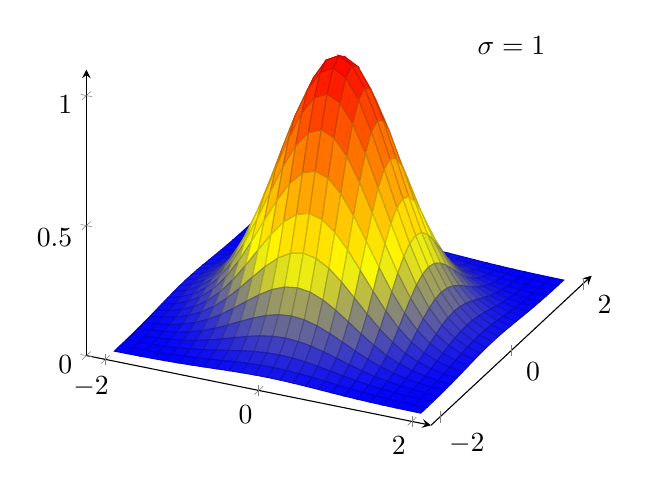
\begin{tikzpicture}

            \begin{axis}[
                    width=8cm,height=8cm,
                    domain=-2:2,
                    xmax=2.25,
                    ymax=2.25,
                    xmin=-2.25,
                    ymin=-2.25,
                    zmax=1.1,
                    axis lines = left,
                    colormap/hot,
                ]

                \addplot3[samples = 25, surf] {exp(-(x^2 + y^2)/1)};
                \node at (rel axis cs:1,0.5,1) [above] {\(\sigma=1\)};

            \end{axis}

        \end{tikzpicture}
    }%
    \quad
    \subfloat{
        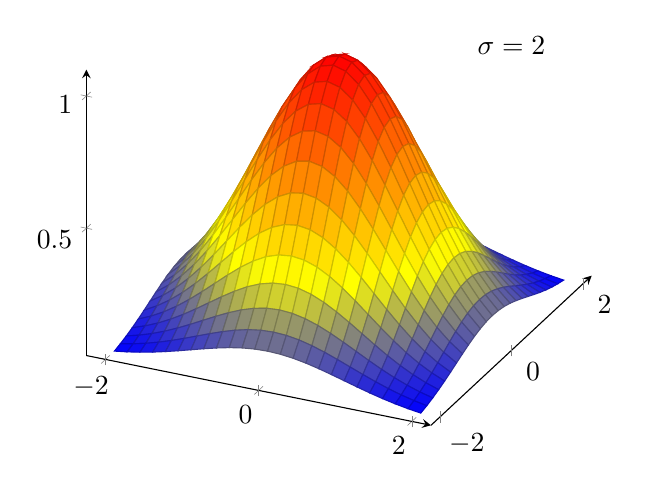
\begin{tikzpicture}

            \begin{axis}[
                    width=8cm,height=8cm,
                    domain=-2:2,
                    xmax=2.25,
                    ymax=2.25,
                    xmin=-2.25,
                    ymin=-2.25,
                    zmax=1.1,
                    axis lines = left,
                    colormap/hot,
                ]

                \addplot3[samples = 25, surf] {exp(-(x^2 + y^2)/2)};
                \node at (rel axis cs:1,0.5,1) [above] {\(\sigma=2\)};

            \end{axis}

        \end{tikzpicture}
    }%
    \caption{A graph of the Gaussian RBF from definition \ref{defe: grbfk} for $d=2$. Evidently, a larger value of $\sigma$ slows the rate of decay increasing the similarity between the same pair of samples.}%
    \label{fig: grbfk_graph_1}
\end{figure}

This kernel is infinitely differentiable meaning it has mean square derivatives of all orders and is therefore very smooth. In fact, some argue that such strong smoothness makes it unrealistic for modelling natural phenomena \cite{RasmussenCarlEdward2006Gpfm,SteinMichaelL1999IoSD}. Nontheless, Gaussian RBF kernelis still the one of the most widely used kernels in literature.

\subsection{Kernel Machines}\label{Section1.4}

In this section, we shall look at two different machine learning models that make use of kernels to perform classification and regression. The first kernel machine we shall look at are support vector machines (SVM). SVMs where originally designed for binary classification and as such we shall only present a model for binary classification, although extensions exist that allow regression and multi-class classification.

For the binary classification problem we are tasked with labelling new samples with either one of two classes, $-1$ or $1$. We shall assume our input space consists of vectors from $\RR^d$ and that we provided with a labelled training set $D = \left\{ \left( \bm{x}_1 , y_1 \right), \left( \bm{x}_1 , y_1 \right), \ldots , \left( \bm{x}_n , y_n \right) \right\}$. One simple method to classify samples is by creating an affine linear hyperplane satisfying
\begin{align} \label{eq: linear_sep_hyp}
    \langle \bm{w}, \bm{x}_i \rangle + b > 0, \quad y_i = +1 \nonumber \\
    \langle \bm{w}, \bm{x}_i \rangle + b < 0, \quad y_i = -1
\end{align}
for some $\bm{w} \in \RR^d$ and $b \in \RR$ where $\norm{w}_2 = 1$. Moreover we would like $\bm{w}$ and $b$ to maximise the margin, that is the maximal distance between the separating hyperplane and the points in $D$. The specific $\bm{w}$ and $b$ obtained through the training set is denoted $\bm{w}_D$ and $b_D$ and the resulting descision function is defined as
\[
    f_D \left( \bm{x} \right) \triangleq \operatorname{sign} \left( \langle \bm{w}_D , \bm{x} \rangle + b_D \right).
\]
There are, however, a number of short comings to this model. The most obvious is that our training data may not be linearly separable in $\RR^d$ meaning that no such $\bm{w}_D$ and $b_D$ exist. Moreover, when noise is introduced to the data set this model will prioritize finding a hyperplane that perfectly separates the two classes, making no comprises in misclassifying points, leaving it subject to overfitting. SVMs where introduced by Boser {\it et al.} \cite{BoserBernhard1992Ataf} to address the first issue of separability. Their approach was to lift the input vector into a more malleable Hilbert space $H_0$ using a feature map. The inputs are then classified within the new space. Unfortunately this method does nothing to address the second issue of over fitting and, if anything, actually worsens it. Cortes and Vapnik \cite{CortesCorinna1995SN} attempted to address this second issue by introducing slack variables to equation \ref{eq: linear_sep_hyp} so that we instead need to satisfy $y_i \left( \langle \bm{w} , \Phi \left( \bm{x}_i \right) \rangle + b \right) \geq 1 - \xi_i$ for some $\xi_i \in \RR_{>0}$. These constraints can be re-written as
\[
    \xi_i \geq 1 - y_i \left( \langle \bm{w} , \Phi \left( \bm{x}_i \right) \rangle + b \right)
\]
and combining this this our slack constraints (that is $\xi_i \geq 0$) yields
\[
    \xi_i \geq \max \left\{ 0, 1 - y_i \left( \langle \bm{w} , \Phi \left( \bm{x}_i \right) \rangle + b \right)  \right\} = L_{\text{hinge}} \left( y_i , \langle \bm{w} , \Phi \left( \bm{x}_i \right) \rangle + b \right)
\]
where $L_{\text{hinge}}$ is the hinge loss defined as
\[
    L_{\text{hinge}} \left( y,\eta \right) \triangleq \max \left\{ 0,1-y\eta \right\}.
\]
This optimization problem can be re-written is the form
\[
    \min_{\left( \bm{w} , b \right) \in H_0 \times \RR} \lambda \norm{\bm{w}}_{H_0} + \frac{1}{n} \sum_{i=1}^{n} L_{\text{hinge}} \left( y_i , f_{\left( \bm{w} , b \right)} \right)
\]
where $f_{\left( \bm{w} , b \right)} : X \to \RR$ is defined as
\[
    f_{\left( \bm{w} , b \right)} \triangleq \langle \bm{w} , \Phi \left( x_i \right) \rangle + b.
\]
Unfortunately, this new embedding requires us to solve for optimal parameters in a very high, or even infinite, dimension vector space. To get around this, often the Lagrange approach is used to solve the corresponding dual problem. When the hinge loss is used the dual problem becomes
\begin{align} \label{eq: SVM_dual_1}
     & \max_{\alpha \in \left[ 0,C \right]^n} \sum_{i=1}^{n} \alpha_i - \frac{1}{2} \sum_{i,j=1}^{n} y_i y_j \alpha_i \alpha_j \langle \Phi \left( \bm{x}_i \right), \Phi \left( \bm{x}_j \right) \rangle \nonumber \\
     & \text{subject to} \quad \sum_{i=1}^{n} y_i \alpha_i = 0
\end{align}
Notice that in the dual problem, we find that inner products are only taken with vectors that have the feature map applied to them allowing us to employ the kernel if the corresponding kernel trick described in section \ref{Section1.1} is known for the feature map used so that \ref{eq: SVM_dual_1} becomes
\begin{align*}
     & \max_{\alpha \in \left[ 0,C \right]^n} \sum_{i=1}^{n} \alpha_i - \frac{1}{2} \sum_{i,j=1}^{n} y_i y_j \alpha_i \alpha_j k \left( \bm{x}_i, \bm{x}_j \right) \\
     & \text{subject to} \quad \sum_{i=1}^{n} y_i \alpha_i = 0.
\end{align*}

The next machine learning model of interest that uses kernels are gaussian processes. To motivate this model, consider the time series data in figure \ref{fig: motive_gp_1}.

\begin{figure}[H]
    \centering
    \subfloat[]{
        \begin{tikzpicture}
            \draw[->,thick] (-0.01,0)--(6,0) node[right]{$x$};
            \draw[->,thick] (0,-0.01)--(0,6) node[above]{$y$};

            \draw[-,ultra thick] (0.7,-0.1)--(0.7,0.1) node[below,yshift=-0.3cm]{$x_1$};
            \draw[fill,draw,blue] (0.7,0.5) circle[radius=2.5pt];

            \draw[-,ultra thick] (1.4,-0.1)--(1.4,0.1) node[below,yshift=-0.3cm]{$x_2$};
            \draw[fill,draw,blue] (1.4,0.6) circle[radius=2.5pt];

            \draw[-,ultra thick] (2.7,-0.1)--(2.7,0.1) node[below,yshift=-0.3cm]{$x_3$};
            \draw[fill,draw,blue] (2.7,1.7) circle[radius=2.5pt];

            \draw[-,ultra thick] (3.7,-0.1)--(3.7,0.1) node[below,yshift=-0.2cm]{$x^{\ast}$};
            \draw[dashed,thick,red] (3.7,0)--(3.7,5);

            \draw[-,ultra thick] (5,-0.1)--(5,0.1) node[below,yshift=-0.3cm]{$x_4$};
            \draw[fill,draw,blue] (5,4) circle[radius=2.5pt];
        \end{tikzpicture}
    }%
    \qquad
    \subfloat[]{
        \begin{tikzpicture}
            \draw[->,thick] (-0.01,0)--(6,0) node[right]{$x$};
            \draw[->,thick] (0,-0.01)--(0,6) node[above]{$y$};

            \draw[-,ultra thick] (0.7,-0.1)--(0.7,0.1) node[below,yshift=-0.3cm]{$x_1$};
            \draw[fill,draw,blue] (0.7,0.5) circle[radius=2.5pt];
            \draw[dashed,blue] (0.7,0)--(0.7,4.7);
            \draw[<->,thick] (0.7,4.7)--(3.7,4.7) node[above,xshift=-1.5cm]{$k(x^{\ast},x_1)$};

            \draw[-,ultra thick] (1.4,-0.1)--(1.4,0.1) node[below,yshift=-0.3cm]{$x_2$};
            \draw[fill,draw,blue] (1.4,0.6) circle[radius=2.5pt];
            \draw[dashed,blue] (1.4,0)--(1.4,3.5);
            \draw[<->,thick] (1.4,3.5)--(3.7,3.5) node[above,xshift=-1.1cm]{$k(x^{\ast},x_2)$};

            \draw[-,ultra thick] (2.7,-0.1)--(2.7,0.1) node[below,yshift=-0.3cm]{$x_3$};
            \draw[fill,draw,blue] (2.7,1.7) circle[radius=2.5pt];
            \draw[dashed,blue] (2.7,0)--(2.7,2.3);
            \draw[<->,thick] (2.7,2.3)--(3.7,2.3) node[above,xshift=-0.9cm]{$k(x^{\ast},x_3)$};

            \draw[-,ultra thick] (3.7,-0.1)--(3.7,0.1) node[below,yshift=-0.2cm]{$x^{\ast}$};
            \node[diamond,draw,fill,draw,red,minimum width = 1cm,minimum height = 1.3cm,scale=0.25] (d) at (3.7,3) {};
            \draw[dashed,thick,red] (3.7,0)--(3.7,5);

            \draw[-,ultra thick] (5,-0.1 )--(5,0.1) node[below,yshift=-0.3cm]{$x_4$};
            \draw[fill,draw,blue] (5,4) circle[radius=2.5pt];
            \draw[dashed,blue] (5,0)--(5,4.5);
            \draw[<->,thick] (3.7,4.5)--(5,4.5) node[above,xshift=-0.3cm]{$k(x^{\ast},x_4)$};
        \end{tikzpicture}
    }%
    \caption{A graph of the Gaussian RBF from definition \ref{defe: grbfk} for $d=2$. Evidently, a larger value of $\sigma$ slows the rate of decay increasing the similarity between the same pair of samples.}%
    \label{fig: motive_gp_1}
\end{figure}

\begin{filecontents*}{./data/gp_intro_dat1.csv}
    x,y0,y1,y2
    0.0,3.8889447299776054,3.252195675396163,2.5723986201044187
    0.10204081632653061,3.8963153731866624,3.2334114175675395,2.4977761527857716
    0.20408163265306123,3.904676475191245,3.2263277175862597,2.4161726074738854
    0.30612244897959184,3.912486422260641,3.2265022294195966,2.3292200441690207
    0.40816326530612246,3.9181367775658873,3.228192583362307,2.2398507798591534
    0.5102040816326531,3.920256370846241,3.2249223304542913,2.152200525625582
    0.6122448979591837,3.9179701155023157,3.2101098230475538,2.071344891386562
    0.7142857142857143,3.9110778971645765,3.1777033459669783,2.0028774256062816
    0.8163265306122449,3.9001283490397016,3.122766415820061,1.9523672809629247
    0.9183673469387755,3.886376053031046,3.04196343041673,1.924753149634383
    1.0204081632653061,3.8716211994498333,2.933909038317024,1.9237443590136485
    1.1224489795918369,3.857954079608229,2.799351626306004,1.9513035606887854
    1.2244897959183674,3.847436905468257,2.6411768356723235,2.0072815139900495
    1.3265306122448979,3.841775787363871,2.4642319083119633,2.0892569830605368
    1.4285714285714286,3.8420321968485376,2.2749858593824617,2.192613833596985
    1.5306122448979593,3.8484268708760094,2.081057401633018,2.310856060666622
    1.6326530612244898,3.8602681088894766,1.8906546442626817,2.436135561712868
    1.7346938775510203,3.876016440194414,1.7119803587951616,2.559934911031695
    1.836734693877551,3.8934729250514666,1.5526570590488398,2.6738332705910244
    1.9387755102040818,3.9100510027824393,1.4192260798320049,2.7702684624537106
    2.0408163265306123,3.9230775813589482,1.3167595333633981,2.8432111425013322
    2.142857142857143,3.9300643637480857,1.248613256762677,2.888679554257369
    2.2448979591836737,3.9289011237509577,1.2163272198562576,2.905046033347129
    2.3469387755102042,3.9179401795449396,1.2196699093041794,2.8931101011392846
    2.4489795918367347,3.8959727008352174,1.2568027645405968,2.855945899531336
    2.5510204081632653,3.8621237371394623,1.3245411459916354,2.7985513820415195
    2.6530612244897958,3.8157151558884888,1.418678279406553,2.7273502460278247
    2.7551020408163267,3.756152285749804,1.5343452363886438,2.6496002463865618
    2.857142857142857,3.682888390340987,1.6663820121189532,2.5727700517645653
    2.9591836734693877,3.595495808498078,1.809697591321269,2.5039341546455005
    3.0612244897959187,3.493850568209357,1.9596010720146781,2.449232028447514
    3.163265306122449,3.378399275439287,2.1120883798539003,2.413420573364779
    3.2653061224489797,3.250456289718835,2.2640650594565668,2.3995428209525658
    3.36734693877551,3.1124629519607803,2.4134903440220477,2.4087275907808734
    3.4693877551020407,2.968139731618476,2.559424609970991,2.4401239977854456
    3.5714285714285716,2.8224826195273596,2.701970562220883,2.4909781807485927
    3.673469387755102,2.6815760504255355,2.8421022219924184,2.556846086350459
    3.7755102040816326,2.5522348648343,2.9813911671556212,2.6319349647504673
    3.8775510204081636,2.441513722741859,3.1216501445256846,2.709555194481732
    3.979591836734694,2.3561485591504203,3.264528290179406,2.7826529438164505
    4.081632653061225,2.3020051023456194,3.4111042700896737,2.8443841134520453
    4.183673469387755,2.2836063990304716,3.5615279847182504,2.8886791623908876
    4.285714285714286,2.3037932704691393,3.7147625310871684,2.9107453218748542
    4.387755102040816,2.3635503438936984,3.8684692167316403,2.907454656505577
    4.4897959183673475,2.461999004872191,4.019063544907245,2.8775731008424583
    4.591836734693878,2.596536742969357,4.161947681776214,2.821805978895311
    4.6938775510204085,2.763082806314141,4.291903941920607,2.742656025464969
    4.795918367346939,2.9563825813547977,4.4036048056748225,2.644116725967176
    4.8979591836734695,3.1703270754187236,4.492179720561176,2.5312380314160974
    5.0,3.398251248127017,4.553760976976619,2.4096316234579827
\end{filecontents*}

\begin{tikzpicture}
    \begin{axis}[
            xmin=-0.0,xmax=6.5,
            ymin=-0.5,ymax=6.5,
            axis line style={draw=none},
            tick style={draw=none},
            yticklabels=\empty,
            xticklabels=\empty,
        ]
        \addplot[smooth, color=black, semithick] table [x=x, y=y0, col sep=comma, mark=none] {./data/gp_intro_dat1.csv};
        \addplot[smooth, color=black, semithick, dashed] table [x=x, y=y1, col sep=comma, mark=none] {./data/gp_intro_dat1.csv};
        \addplot[smooth, color=black, semithick, dotted] table [x=x, y=y2, col sep=comma, mark=none] {./data/gp_intro_dat1.csv};
    \end{axis}
    \draw[->,thick] (0,0.5)--(0,5.5) node[above]{$y$};
    \draw[->,thick] (0,0.5)--(6,0.5) node[right]{$x$};
\end{tikzpicture}


\subsection{Gaussian Processes for Regression}\label{Section1.5}

We saw in section \ref{Section1.4} that, unlike most other machine learning models, GPs infer over a distribution of functions $p \left( f \mid D \right)$ instead of a vector of parameteric values $p \left( \bm{\theta} \mid D \right)$. Naively, one may attempt to find a suitable $f$ by fixing a class of functions $\calF$ and then search over this class to find a function that best represents the data. However, this may not work well if there is not enough richness in $\calF$ to represent the data. Instead we choose a suitable $f$ by assigning a prior probability to every possible function using the training data and then to select the function with the highest probability. To keep this computation tractable we only evalute our predicted function at a finite number of points. The prediction itself is found by taking the mean over all functions with respect to the posterior conditioned on the observed data which is assumed to be jointly Gaussian with the input value. This gives rise to Gaussian Process more formally stated in definition \ref{defe: GP}.

\begin{defe}[Gaussian Process] \label{defe: GP}
    A Gaussian Process (GP) is a collection of random variables with index set $I$, such that every finite subset of random variables has a joint Gaussian distribution \cite{RasmussenCarlEdward2006Gpfm,MurphyKevinP2012Ml}.
\end{defe}

A GP is completely characterised by a mean function $m(\bm{x})$ and a kernel, which in the context of GPs is sometimes called a covariance function, $k (\bm{x}, \bm{x'})$ on a real process as
\begin{align*}
    m(\bm{x})           & = \EE \left[ f(\bm{x}) \right]                                         \\
    k (\bm{x}, \bm{x'}) & = \EE \left[ (f(\bm{x}) - m(\bm{x})) (f(\bm{x'}) - m(\bm{x'})) \right]
\end{align*}
GPs define a prior over all possible functions which can be used to create a posterior once enough data has been observed. The prior is used to represent the functions we expect to see before any observations are made. Although defining a prior over all possible function may seem computationally intractable, we actually only need to define a distribution over a finite number of points. Before any observations are made, we typically assume that the mean function is the constant zero function, that is $m \left( \bm{x} \right) = 0$. A function $f(\bm{x})$ sampled from a GP with mean $m(\bm{x})$ and covariance $k (\bm{x}, \bm{x'})$ is written as
\[
    f(\bm{x}) \sim \calG \calP \left( m(\bm{x}), k (\bm{x}, \bm{x'}) \right)
\]
Since a GP is a collection of random variables it must satisfy the consistency requirement, that is, an observation of a set of variables should not the distribution of any small sub set of the observed values. More specifically if
\[
    (\bm{y_1}, \bm{y_2}) \sim \calN (\bm{\mu}, \bm{\Sigma})
\]
then
\begin{align*}
    \bm{y_1} & \sim \calN (\bm{\mu_1}, \bm{\Sigma_{1,1}}) \\
    \bm{y_2} & \sim \calN (\bm{\mu_2}, \bm{\Sigma_{2,2}})
\end{align*}

where $\bm{\Sigma_{1,1}}$ and $\bm{\Sigma_{2,2}}$ are the relevant sub matrices. Again, we shall us the notation that for set of data $\bm{W} = \left[ \bm{w}_1 ,\bm{w}_2 , \ldots , \bm{w}_n \right]^{\intercal} \in \RR^{n \times d}$ and $\bm{W}' = \left[ \bm{w}_1' ,\bm{w}_2' , \ldots , \bm{w}_m' \right]^{\intercal} \in \RR^{n' \times d}$ we use the notation
\[
    \left( \bm{K}_{\bm{W} \bm{W}'} \right)_{i,j} \triangleq k \left( \bm{w}_i , \bm{w}_j' \right)
\]
where \( \bm{K}_{\bm{W} \bm{W}'} \in \RR^{n \times n'} \). The convariance function completely characterized by its kernel. Unless otherwise stated, the kernel or covariance function used in examples and experimentation in the Gaussian RBF kernel, definition \ref{defe: grbfk}. To understand this better, as a small exercise we can select a number of inputs $\bm{X}^{\star} = \left[ \bm{x}_1 , \bm{x}_2 , \ldots , \bm{x}_{n^{\star}} \right]^{\intercal} \in \RR^{n^{\star} \times d}$ of compute the corresponding covariance matrix using the Gaussian RBF kernel. Gaussian vectors can then be sampled using a joint Gaussian distribution using the covariance matrix from the distribution
\[
    \bm{f}^{\star} \sim \calN \left( \bm{0}, \bm{K_{X^{\star} X^{\star}}} \right)
\]
graph its values as a function of its inputs.

\begin{filecontents*}{./data/gp_intro_dat1.csv}
    x,y0,y1,y2
    0.0,2.6341780930873786,4.41685044685407,1.884123117075101
    0.11224489795918367,2.685150340856032,4.351109330694541,2.0933788453347146
    0.22448979591836735,2.758222906849677,4.246986054733594,2.3215583495507697
    0.336734693877551,2.844091796198551,4.111722477611423,2.5621308980348045
    0.4489795918367347,2.9327004798948444,3.954138391914307,2.8093607381581323
    0.5612244897959183,3.0142490315111,3.7837568463624893,3.058296829896802
    0.673469387755102,3.0800293333419133,3.609905398833131,3.304575221937234
    0.7857142857142857,3.1230071846450134,3.4408573216000065,3.5440886761610075
    0.8979591836734694,3.1381275068842287,3.2830844115325393,3.772606115615495
    1.010204081632653,3.1223796951701805,3.1407028040204787,3.985434762859824
    1.1224489795918366,3.074690487867501,3.0151840031490704,4.177213384641246
    1.2346938775510203,2.99572649694323,2.9053883056890326,4.341906534238328
    1.346938775510204,2.887680093346262,2.807934404050683,4.473021654529128
    1.4591836734693877,2.7540712359611135,2.7178753181761683,4.5640359352552755
    1.5714285714285714,2.5995639802641644,2.629596908378246,4.608968085491204
    1.683673469387755,2.4297636797240854,2.537815790076743,4.603008456947798
    1.7959183673469388,2.250945266539242,2.4385306514757277,4.54310273176884
    1.9081632653061225,2.0696826217289814,2.3297825969976156,4.428402138611055
    2.020408163265306,1.8923794707563157,2.2121155584786374,4.26051300065903
    2.13265306122449,1.724750314129252,2.088670901030661,4.043522033936433
    2.2448979591836733,1.5713409480295042,1.9649185604698398,3.78380984825793
    2.357142857142857,1.4351902937232137,1.8480772970914263,3.4896953544368947
    2.4693877551020407,1.3177316537250037,1.7463209648090843,3.170973707657322
    2.5816326530612246,1.2189781885886188,1.667887909534986,2.838411584600058
    2.693877551020408,1.137982180009872,1.6202034591848866,2.503253609595508
    2.806122448979592,1.0734814750833834,1.6091067041507867,2.176777775544475
    2.9183673469387754,1.0246008560812094,1.638242628202587,1.8699164299237567
    3.0306122448979593,0.9914469543413351,1.708653796550625,1.5929463528940093
    3.142857142857143,0.9754532832118712,1.8185871450769515,1.3552308689036683
    3.2551020408163267,0.9793831046385866,1.9635250522558478,1.1649988273056024
    3.36734693877551,1.0069633897912214,2.136445411268843,1.0291341361289352
    3.479591836734694,1.0622134340832736,2.328310102622806,0.9529576266820667
    3.5918367346938775,1.1485904962060034,2.5287676666005745,0.9399816624503701
    3.704081632653061,1.2681182060719118,2.7270230125223396,0.9916380696381344
    3.816326530612245,1.4206777569266578,2.9127943188682153,1.1069890129419622
    3.9285714285714284,1.603600797665261,3.077239529790242,1.282461239660869
    4.040816326530612,1.8116633596458505,3.213718985997705,1.5116563075035667
    4.153061224489796,2.0374945244629954,3.31826875093589,1.7853109321561014
    4.26530612244898,2.272346385818944,3.3896996920659737,2.0914743830547122
    4.377551020408164,2.50710273056381,3.4293088690936613,2.415953795652976
    4.489795918367347,2.7333622652331386,3.440263336916595,2.743037053839629
    4.6020408163265305,2.9444150750492786,3.426788503862636,3.0564529194286605
    4.714285714285714,3.1359501955059153,3.3933321658244284,3.3404756976868217
    4.826530612244898,3.306372509617609,3.343882098004392,3.5810500536442835
    4.938775510204081,3.456677113806286,3.281564998201946,3.766794718394943
    5.051020408163265,3.5899014357864862,3.2085942528948497,3.889767236618262
    5.163265306122449,3.710253447229357,3.1265441378249808,3.9459164775264113
    5.275510204081633,3.822067924064683,3.036856306931041,3.9352029543435254
    5.387755102040816,3.928774395166681,2.9414323013414645,3.8614290770863415
    5.5,4.032057566247807,2.843156622782664,3.7318467351526268
\end{filecontents*}

\begin{filecontents*}{./data/gp_intro_dat2.csv}
    x,mu,y0,y1,y2,bU,bL
    0.0,2.96787109791578,3.646442446207024,2.3796779884645356,3.123887098083909,3.8222957144465917,2.1134464813849685
    0.11224489795918367,3.178846435851742,3.7278533056947927,2.705139783400845,3.3197136652913843,3.8425540443223007,2.515138827381183
    0.22448979591836735,3.373957062754166,3.772122911137243,3.033674383762561,3.4864096188544065,3.8416203985733905,2.906293726934942
    0.336734693877551,3.550670833185919,3.7845706480846375,3.3482893361633472,3.6227538754415383,3.8226477418327116,3.2786939245391267
    0.4489795918367347,3.707387470227142,3.777024821961083,3.6497714076425667,3.734021204276469,3.7908281722625117,3.623946768191772
    0.5612244897959183,3.8435001880813098,3.7587623765632605,3.9224326540622303,3.820415281746996,3.938789896922746,3.7482104792398734
    0.673469387755102,3.959374699757277,3.7401691473547714,4.161761533893699,3.884187912930478,4.2112638754378935,3.70748552407666
    0.7857142857142857,4.056245238332488,3.727886967246087,4.3591514373501585,3.9294944134700884,4.440290931214802,3.6721995454501735
    0.8979591836734694,4.136035742591053,3.7320230213633776,4.516870894977162,3.9667169440013335,4.6225623417878845,3.6495091433942224
    1.010204081632653,4.201122318895088,3.7511336294964686,4.631536079365145,3.9909291094494637,4.756943867968448,3.645300769821728
    1.1224489795918366,4.254059537569402,3.7922886212348805,4.703821106353732,4.014456904551665,4.844164391874928,3.663954683263876
    1.2346938775510203,4.297297268072625,3.8510310641448773,4.736836098027459,4.040882180292408,4.886718646421257,3.7078758897239927
    1.346938775510204,4.332916090251523,3.931146658869461,4.737917134427073,4.0721402987298845,4.8886932140093196,3.7771389664937254
    1.4591836734693877,4.362407665942143,4.019692223676497,4.711145152040588,4.114354849026403,4.855508162034269,3.869307169850018
    1.5714285714285714,4.386522000140943,4.113994631302509,4.667147410140193,4.1675113923767135,4.79358919579317,3.9794548044887157
    1.683673469387755,4.405196773426522,4.211161115648332,4.60858632272203,4.2301483229724735,4.709995085814498,4.100398461038546
    1.7959183673469388,4.417575648333239,4.297237502243545,4.542647493156313,4.298601004588312,4.612045273426419,4.223106023240059
    1.9081632653061225,4.422113551855313,4.370044631852721,4.478504417000914,4.366233750854552,4.507185391473455,4.337041712237171
    2.020408163265306,4.416758358107319,4.4212535412567835,4.413073469318789,4.428720525173312,4.439002309014812,4.394514407199825
    2.13265306122449,4.399191007367498,4.4498214644109035,4.354633815643454,4.472837424274621,4.501454599238494,4.296927415496501
    2.2448979591836733,4.367100601462363,4.44669502086167,4.293220973455457,4.495071115055989,4.529355328572067,4.204845874352659
    2.357142857142857,4.318467882753287,4.4122754488830465,4.2367626348642995,4.480392701402552,4.511998980020114,4.124936785486461
    2.4693877551020407,4.251829947856004,4.344361140161457,4.176480274188317,4.420872228223025,4.444440701959786,4.059219193752223
    2.5816326530612246,4.166501022807468,4.242712341391929,4.110274997773214,4.315673648503417,4.324777879750019,4.008224165864918
    2.693877551020408,4.062728357957119,4.110217875771083,4.032563200602017,4.153918593320322,4.154406402240164,3.9710503136740742
    2.806122448979592,3.9417683270387145,3.9492135726749384,3.9344120355000705,3.9443400697750968,3.9571937560826638,3.926342897994765
    2.9183673469387754,3.805875044263767,3.7642279401126544,3.810832282328448,3.684817080524404,3.9345310053498097,3.6772190831777247
    3.0306122448979593,3.6582015833339296,3.564842924761986,3.6644624038944493,3.3833530964865193,3.9269741902831705,3.3894289763846888
    3.142857142857143,3.5026215163692607,3.3520647108430026,3.488370188345563,3.052946676019309,3.9234237680191817,3.0818192647193396
    3.2551020408163267,3.3434853499709174,3.1402141378498163,3.2837887833202726,2.7002390009588226,3.920293063216916,2.7666776367249186
    3.36734693877551,3.1853319635639767,2.934150639260623,3.057322775625835,2.3472996257286054,3.914233966397971,2.4564299607299827
    3.479591836734694,3.03257891484487,2.738827249921258,2.812094834179371,2.009196676123942,3.902114762761585,2.163043066928155
    3.5918367346938775,2.8892171796754873,2.5662919443248073,2.559707152254641,1.6967015390942675,3.881056263819646,1.8973780955313282
    3.704081632653061,2.758535417727554,2.41434042449297,2.309411800258502,1.4256334316849872,3.848437973565799,1.668632861889309
    3.816326530612245,2.642896256015177,2.2902148380401837,2.075552115650442,1.207890471342624,3.8018786148254615,1.4839138972048924
    3.9285714285714284,2.5435825902305362,2.1965744091641124,1.8662299680038845,1.0467598332277432,3.7392081008329594,1.3479570796281128
    4.040816326530612,2.4607259083694415,2.133954232173078,1.6922651032951084,0.952486845042865,3.6584498086819774,1.2630020080569058
    4.153061224489796,2.393321664023437,2.0881938587934696,1.566133253333461,0.92147130773977,3.5578289289014684,1.2288143991454055
    4.26530612244898,2.339329380270647,2.0632588371219063,1.4903968555363714,0.94987473663854,3.435816329632721,1.2428424309085735
    4.377551020408164,2.295848100924048,2.0605594124527933,1.4690236774181895,1.033187881225276,3.2912091804701387,1.3004870213779576
    4.489795918367347,2.259351656203322,2.064341290936802,1.499164363108256,1.1636813952423448,3.123241143061824,1.3954621693448201
    4.6020408163265305,2.2259635269573055,2.0739080755801877,1.575649936757477,1.3294049093439706,2.931708042701583,1.520219011213028
    4.714285714285714,2.1917482915683912,2.0845379827266677,1.6904928495001776,1.5224847717101069,2.717092081155121,1.6664045019816616
    4.826530612244898,2.1529959577040843,2.0900622587437008,1.8320811599608942,1.733755447747318,2.4806793091811996,1.8253126062269691
    4.938775510204081,2.10647694342231,2.087733094036374,1.98722071801456,1.9517354055585423,2.2248945171189956,1.988059369725624
    5.051020408163265,2.049648890548753,2.0747166503580527,2.1438285289379833,2.167467964578078,2.149507699667685,1.9497900814298208
    5.163265306122449,1.9808014834652514,2.050810263655156,2.283421101970534,2.3742039664111614,2.297682746932975,1.663920219997528
    5.275510204081633,1.8991314699538484,2.006424555553889,2.395089681917207,2.5656201066053885,2.429871221330997,1.3683917185766998
    5.387755102040816,1.8047465055032903,1.9408588788404912,2.4682291512970815,2.7418915989000654,2.5411728761483077,1.068320134858273
    5.5,1.69860261545027,1.8531818596862015,2.488627885130089,2.8888780190386125,2.628636682030301,0.7685685488702394
\end{filecontents*}

\begin{figure}[h]
    \centering
    \subfloat[]{
        \begin{adjustbox}{width=0.48\textwidth}
            \begin{tikzpicture}[>=latex]
                \begin{axis}[
                        xmin=-0.0,xmax=6.5,
                        ymin=-0.5,ymax=6.5,
                        axis line style={draw=none},
                        tick style={draw=none},
                        yticklabels=\empty,
                        xticklabels=\empty,
                    ]
                    \addplot[smooth, color=black, semithick] table [x=x, y=y0, col sep=comma, mark=none] {./data/gp_intro_dat1.csv};
                    \addplot[smooth, color=black, semithick, dashed] table [x=x, y=y1, col sep=comma, mark=none] {./data/gp_intro_dat1.csv};
                    \addplot[smooth, color=black, semithick, dotted] table [x=x, y=y2, col sep=comma, mark=none] {./data/gp_intro_dat1.csv};

                    \addplot[name path = bU, mark=none, blue!10] coordinates {(0,0.5) (5.5,0.5)};
                    \addplot[name path = bL, mark=none, blue!10] coordinates {(0,5.75) (5.5,5.75)};
                    \addplot [blue!10] fill between [of = bU and bL, soft clip={domain=0:5.5}];

                \end{axis}
                \draw[color=red, ultra thick] (0,3)--(5.8,3);
                \draw[->,thick] (0,0.5)--(0,5.5) node[above]{$y$};
                \draw[->,thick] (0,0.5)--(6,0.5) node[right]{$x$};
            \end{tikzpicture}
        \end{adjustbox}
    }
    \subfloat[]{
        \begin{adjustbox}{width=0.48\textwidth}
            \begin{tikzpicture}[>=latex]
                \begin{axis}[
                        xmin=-0.0,xmax=6.5,
                        ymin=-0.5,ymax=6.5,
                        axis line style={draw=none},
                        tick style={draw=none},
                        yticklabels=\empty,
                        xticklabels=\empty,
                    ]
                    \addplot[smooth, color=black, semithick] table [x=x, y=y0, col sep=comma, mark=none] {./data/gp_intro_dat2.csv};
                    \addplot[smooth, color=black, semithick, dashed] table [x=x, y=y1, col sep=comma, mark=none] {./data/gp_intro_dat2.csv};
                    \addplot[smooth, color=black, semithick, dotted] table [x=x, y=y2, col sep=comma, mark=none] {./data/gp_intro_dat2.csv};
                    \addplot[smooth, color=red, ultra thick] table [x=x, y=mu, col sep=comma, mark=none] {./data/gp_intro_dat2.csv};

                    \addplot[name path = bU, smooth, color=blue!10] table [x=x, y=bU, col sep=comma, mark=none] {./data/gp_intro_dat2.csv};
                    \addplot[name path = bL, smooth, color=blue!10] table [x=x, y=bL, col sep=comma, mark=none] {./data/gp_intro_dat2.csv};
                    \addplot [blue!10] fill between [of = bU and bL, soft clip={domain=0:5.5}];
                \end{axis}
                \draw[->,thick] (0,0.5)--(0,5.5) node[above]{$y$};
                \draw[->,thick] (0,0.5)--(6,0.5) node[right]{$x$};
                \draw[-,ultra thick] (0.5,0.4)--(0.5,0.6) node[below,yshift=-0.3cm]{$x_1$};
                \draw[-,ultra thick] (2.1,0.4)--(2.1,0.6) node[below,yshift=-0.3cm]{$x_2$};
                \draw[-,ultra thick] (2.95,0.4)--(2.95,0.6) node[below,yshift=-0.3cm]{$x_3$};
                \draw[-,ultra thick] (5.3,0.4)--(5.3,0.6) node[below,yshift=-0.3cm]{$x_4$};

                \foreach \Point in {(0.5, 3.45), (2.1, 4.0), (2.95, 3.6), (5.3, 2.1)}{
                        \node at \Point {\contour{white}{\Large \textbf{+}}};
                    }
            \end{tikzpicture}
        \end{adjustbox}
    }
    \caption{Panel (A) shows three function drawn from the prior distribution. Panel (B) shows three function drawn from the prior distribution after four observations have been made. In both panels the mean function is drawn in red, sampled functions in black and twice the standard deviation shaded in light blue.}
    \label{fig: GP_func_samples}
\end{figure}

Figure \ref{fig: GP_func_samples} (A) shows three samples drawn from the prior before any observations are made. GPs also allow us to compute the pointwise variance which can provide some measure of variability for predicted values. The blue shaded area of figure \ref{fig: GP_func_samples} (A) represents twice the standard deviation about the mean.

\subsubsection{Noise-free observations}\label{Section1.5.1}
Typically when using GP we would like to incorporate data from observations, or training data, into our predictions on unobserved values.
Let us suppose there is some obsevered data $D = \left\{ (\bm{x}_i, \bm{f}_i) \mid i \in \left\{ 1,2, \ldots , n \right\} \right\}$ which is (unrealistically) noise-free that we would like to model as a GP. In other words, for any sample in our dataset we can be certain that the observed value is the true value of the underlying function we wish to model. Then for the observed data
\[
    \bm{f} \sim \calN \left( \bm{0}, \bm{K_{XX}} \right).
\]
We would then like to make a prediction for unobserved values say $X^{\star} = \left[ \bm{x}_1^{\star}, \bm{x}_2^{\star}, \ldots , \bm{x}_{n_\star}^{\star} \right]$ with value $f_{\star}$ as has a distribution of
\[
    \bm{f}_{\star} \sim \calN \left( \bm{0}, \bm{K_{X^{\star}X^{\star}}} \right).
\]
where $\bm{K_{X^{\star}X^{\star}}} = k(\bm{X^{\star}}, \bm{X^{\star}}) \in \RR^{n_\star \times n_\star}$. Here $\bm{f}$ and $\bm{f}_{\star}$ are independent but we would like to give them some sort of correlation. We can do this by having them originate from the same joint distribution. According to the prior, we can write the joint distribution of the training points $\bm{f}$ and the test points $\bm{f}_{\star}$ as
\[
    \begin{bmatrix}
        \bm{f} \\
        \bm{f}_{\star}
    \end{bmatrix}
    \sim \calN
    \begin{pmatrix}
        \bm{0}, &
        {
                \begin{bmatrix}
                    \bm{K_{XX}}                     & \bm{K_{XX^{\star}}}         \\
                    \bm{K_{XX^{\star}}}^{\intercal} & \bm{K_{X^{\star}X^{\star}}}
                \end{bmatrix}
            }
    \end{pmatrix}
\]
where $\bm{K_{XX^{\star}}} = k(\bm{X}, \bm{X^{\star}}) \in \RR^{n \times n_\star}$.

While the above does give us some information on $\bm{f}_{\star}$ is related to the observed data and the test inputs, it does not provide any method to evalute $\bm{f}_{\star}$. To do this we shall need the assistance of the following lemma
\begin{thm}\label{theorem: cond_of_MVN}
    (Marginals and conditionals of an MVN \cite{MurphyKevinP2012Ml}) Suppose $\bm{x} = (\bm{x}_1, \bm{x}_2)$ is jointly Gaussian with parameters
    \[
        \bm{\mu} =
        \begin{bmatrix}
            \bm{\mu}_1 \\
            \bm{\mu}_2
        \end{bmatrix}, \quad
        \bm{\Sigma} =
        \begin{bmatrix}
            \bm{\Sigma}_{1,1} & \bm{\Sigma}_{1,2} \\
            \bm{\Sigma}_{2,1} & \bm{\Sigma}_{2,2}
        \end{bmatrix}
    \]
    then the posterior conditional is given by
    \begin{align*}
        \bm{x}_2 \mid \bm{x}_1 & \sim \calN \left( \bm{x}_2 \mid \bm{\mu}_{2 \mid 1}, \bm{\Sigma}_{2 \mid 1} \right)          \\
        \bm{\mu}_{2 \mid 1}    & = \bm{\mu}_2 + \bm{\Sigma}_{2,1} \bm{\Sigma}_{1,1}^{-1} \left( \bm{x}_1 - \bm{\mu}_1 \right) \\
        \bm{\Sigma}_{2 \mid 1} & = \bm{\Sigma}_{2,2} - \bm{\Sigma}_{2,1} \bm{\Sigma}_{1,1}^{-1} \bm{\Sigma}_{1,2}
    \end{align*}
\end{thm}

Thus finding a mean an covariance for $\bm{f}_{\star}$ requires a direct application of Theorem \ref{theorem: cond_of_MVN} which gives
\begin{align*}
    \bm{f}_{\star} \mid \bm{K_{XX^{\star}}} , \bm{K_{XX}}, \bm{f} \sim \calN \left( \bm{\mu}^{\star}, \bm{\Sigma}^{\star} \right)
\end{align*}
where
\begin{align*}
    \bm{\mu}^{\star} & = \bm{0} + \bm{K_{XX^{\star}}}^{\intercal} \bm{K_{XX}}^{-1} \left( \bm{f} - \bm{0} \right) \\
                     & = \bm{K_{XX^{\star}}}^{\intercal} \bm{K_{XX}}^{-1} \bm{f}
\end{align*}
and
\begin{align*}
    \bm{\Sigma}^{\star} & = \bm{K_{X^{\star}X^{\star}}} - \bm{K_{XX^{\star}}}^{\intercal} \bm{K_{XX}}^{-1} \bm{K_{XX^{\star}}}
\end{align*}
meaning we can write a distribution for $\bm{f}_{\star}$ as
\begin{equation}\label{prop:GP_train_distr1}
    \bm{f}_{\star} \mid \bm{K_{XX^{\star}}} , \bm{K_{XX}}, \bm{f} \sim \calN \left( \bm{K_{XX^{\star}}}^{\intercal} \bm{K_{XX}}^{-1} \bm{f},  \bm{K_{X^{\star}X^{\star}}} - \bm{K_{XX^{\star}}}^{\intercal} \bm{K_{XX}}^{-1} \bm{K_{XX^{\star}}}  \right)
\end{equation}
Function values from the unobserved inputs $\bm{X^{\star}}$, that is $\bm{f}_{\star}$, can be estimated using the joint posterior distribution by evaulting the mean of \ref{prop:GP_train_distr1}. Figure \ref{fig: GP_func_samples} (B) shows these computations given a data set $D = \left\{ \left( x_1 , y_1 \right) , \left( x_2 , y_2 \right) , \left( x_3 , y_3 \right) , \left( x_4 , y_4 \right) \right\}$. Notice that the variance tightens around the observed values since (assuming no noise in our data is present) we know for certain this is how our target function should behave at $x_1,x_2,x_3$ and $x_4$. Specifying the properties of the prior is important since it fixes the properties of the functions considered during inference.

\subsubsection{Prediction with Noisy observations}\label{Section1.5.2}
When attempting to model our value function we usually do not have access to the value function itself but a noisy version thereof, $y = f(\bm{x}) + \varepsilon$ where $\varepsilon \sim \calN (0, \sigma_n^2)$ meaning the prior on the noisy values becomes
\[
    \operatorname{cov} (\bm{y}) = \bm{K_{XX}} + \sigma_n^2 \bm{I}
\]
The reason why noise is only added along the diagonal follows from the assumption of independence in our data.
We can write out the new distribution of the observed noisy values along the points at which we wish to test the underlying function as
\[
    \begin{bmatrix}
        \bm{y} \\
        \bm{f}_{\star}
    \end{bmatrix}
    \sim \calN
    \begin{pmatrix}
        \bm{0}, &
        {
                \begin{bmatrix}
                    \bm{K_{XX}} + \sigma_n^2 \Id_{n \times n} & \bm{K_{XX^{\star}}}         \\
                    \bm{K_{XX^{\star}}}^{\intercal}           & \bm{K_{X^{\star}X^{\star}}}
                \end{bmatrix}
            }
    \end{pmatrix}
\]
Using a similar we arrive at a similar condition distribution of $\bm{f}_{\star} \mid \bm{K_{XX^{\star}}} , \bm{K_{XX}}, \bm{f}$ we arrive at one of the most fundamental equations for GP regression tasks
\begin{equation}\label{prop:GP_train_distr2}
    \bm{f}_{\star} \mid \bm{K_{XX^{\star}}} , \bm{K_{XX}}, \bm{y} \sim \calN \left( \overline{\bm{f}_{\star}}, \operatorname{cov} (\bm{f}_{\star}) \right)
\end{equation}
where
\begin{align}
    \overline{\bm{f}_{\star}}           & \triangleq \bm{K_{XX^{\star}}}^{\intercal} \left[ \bm{K_{XX}} + \sigma_n^2 \Id_{n \times n} \right]^{-1} \bm{y} \label{eq: GP_train_distr2_mean}                                  \\
    \operatorname{cov} (\bm{f}_{\star}) & = \bm{K_{X^{\star}X^{\star}}} - \bm{K_{XX^{\star}}}^{\intercal} \left[ \bm{K_{XX}} + \sigma_n^2 \Id_{n \times n} \right]^{-1} \bm{K_{XX^{\star}}} \label{eq: GP_train_distr2_var}
\end{align}
Remarkably, this gives us the the exact same posterior distribution ascertained from the weight space derivation in equation \ref{eq: comput_f_ast_3}. Notice that the prediction of the mean in equation \ref{eq: GP_train_distr2_mean} is a linear combination of the observations, somtimes referred to as a {\it linear predictor}. Another way of looking at the prediction is seeing it as a linear combination of $n$ kernel evaluations centered at the input $\bm{x}^{\star}$
\[
    \bm{f}_{\star} = \sum_{i=1}^{n} \alpha_i k \left( \bm{x}_i , \bm{x}^{\ast} \right)
\]
where $\bm{\alpha} = \left[ \bm{K_{XX}} + \sigma_n^2 \Id_{n \times n} \right]^{-1} \bm{y}$. Intuitively, this expression can be understood by realising that despite defining the GP defining a joint Gaussian distribution over the observations when making predictions GPs only require the $(n+1)$-dimension distribution defined by the $n$ observations and the single test point. Marginalising by taking  the relevant submatrix block of the covariance matrix yields our desired $1$-dimensional prediction.

Also notice that the covariance does not depend on observations but scales quadratically to the norm of the testing inputs. This is a key feature of GPs. The variance is comprised of the difference between the prior covariance, $\bm{K_{X^{\star}X^{\star}}}$, and positive term $\bm{K_{XX^{\star}}}^{\intercal} \left[ \bm{K_{XX}} + \sigma_n^2 \Id_{n \times n} \right]^{-1} \bm{K_{XX^{\star}}}$ which represents knowledge given by the observations about the underlying function.

Algorithm \ref{alg: Unoptimized_GPR} shows one possible implementation for computing the mean and covariance of a single test input.

    {\centering
        \begin{minipage}{.85\linewidth}
            \begin{algorithm}[H]
                \caption{Unoptimized GPR}
                \label{alg: Unoptimized_GPR}
                \SetAlgoLined
                \DontPrintSemicolon
                \SetKwInOut{Input}{input}\SetKwInOut{Output}{output}

                \Input{Observations $\bm{X}, \bm{y}$ and a test input $\bm{x}^{\star}$.}
                \Output{A prediction $\overline{f_{\star}} $ with its corresponding variance $ \VV \left[ f_{\star} \right]$.}
                \BlankLine
                $\bm{L} = \operatorname{cholesky} \left( \bm{K_{XX}} + \sigma_n^2 \Id_{n \times n} \right)$\;
                $\bm{\alpha} = \operatorname{lin-solve} \left( \bm{L}^{\intercal} , \operatorname{lin-solve} \left( \bm{L}, \bm{y} \right) \right)$\;
                $\overline{f_{\star}} = \bm{K_{x^{\star} X}} \bm{\alpha}$\;
                $\bm{v} = \operatorname{lin-solve} \left( \bm{L}, \bm{K_{x^{\star} X}} \right)$\;
                $\VV \left[ f_{\star} \right] = \bm{K_{x^{\star} x^{\star}}} - \bm{v}^{\intercal} \bm{v}$\;
                \Return{$\overline{f_{\star}} , \VV \left[ f_{\star} \right]$}
                \BlankLine
            \end{algorithm}
        \end{minipage}
        \par
    }

A cholesky decomposition is typically used since $\bm{L}$ can be used twice to assist in solving both the linear systems in the mean and covariance. Unfortunately, a cholesky decomposition incurres a runtime of $\calO \left( n^3 \right)$ where $n$ is the number of samples making it impractical for large data sets. In the later chapters we shall consider other methods for solving these linear systems.
\newpage

% \section{Hecke Algebras Generated by a Coxeter Group}\label{Chapter3}
% The purpose of this section is to investigate the Hecke algebra obtained when we choose $G=\SL_n(\FF_q)$ and $K=B(\FF_q)$, the Borel subgroup of $G$, i.e.\ the subgroup of upper-triangular matrices in $G$.
% For this chapter, our convolution product associated to $\calH$ is modified with a normalising factor $\frac{1}{|B|}$.
% We begin in Section \ref{Section3.1} by investigating the Weyl group of $G$.
% We give its general definition and show that it reduces to the symmetric group $S_n$ for our purposes.
% Next, in Section \ref{Section3.2}, we thoroughly describe the algebra $\calH(G,B)$ in the simple case of $G=\SL_2(\FF_q)$.
% We move to the more difficult cases of $G=\SL_3(\FF_q)$ and $G=\SL_4(\FF_q)$ in Sections \ref{Section3.3} and \ref{Section3.4} respectively.
% These examples lead us to the definition of a Coxeter group, given in Section \ref{Section3.5}.
% This chapter is concluded with the definition of a Hecke algebra of a finite Coxeter group and a complete description of $\calH(G,B)$ in the general case.
% This is done so in Section \ref{Section3.6}.

% %%%%%%%%%%%%%%%%%%%%%%%%%%%%%%%%%%%%%%%%%%%%%%%%%%%%%%%%%%%%%%%%%%%%%%%%%%%%%%%%%%%%%%%%%%%%%%

% \subsection{The Weyl group $W$}\label{Section3.1}
% Fix the group $G=\GL_n(\FF_q)$.
% Consider the subgroup of diagonal matrices
% \[
% 	T := \{\diag(a_1,\ldots,a_n)\ |\ a_i\in\FF_q^\times\}\subseteq G.
% \]
% This is a \emph{maximal torus} of $G$.
% The \emph{Weyl group} of $G$ is defined as the quotient group $W := N_G(T)/T$, where $N_G(T) := \{t\in T\ |\ gTg^{-1}=T\}$ is the \emph{normaliser} of $T$ in $G$.
% The Weyl group may be understood as the reflection group of the \emph{root system} associated to a Lie group $G$.
% It is a useful fact in \cite{Brocker85} that all maximal tori are conjugate to each other over the algebraic closure of $\FF_q$.
% As a result, $W$ is independent of the choice of maximal tori, so we only need to consider the one we have chosen.

% Our goal in this section is to show that $W\cong S_n$.
% To do this, we need a lemma.

% \begin{lem}\label{lemma: normaliser_is_generalised_permutation_matrices}
% 	$N_G(T)$ is the set of monomial matrices in $G$.
% \end{lem}

% Before we prove the lemma, we need a definition and a small fact about matrices.
% The \emph{spectrum} of a matrix is the multiset of its eigenvalues.
% The fact we need is that conjugation preserves the spectrum of a matrix.
% More specifically, for any $A,B\in G$, the spectrums of $A$ and $BAB^{-1}$ coincide.
% To see this, notice
% \[
% 	\det(BAB^{-1}-\lambda I) = \det(BAB^{-1}-\lambda BB^{-1}) = \det(B)\det(A-\lambda I)\det(B^{-1}) = \det(A-\lambda I).
% \]
% We see that $A$ and $BAB^{-1}$ have the same characteristic polynomial which proves the fact.

% \begin{proof}[Proof of Lemma \ref{lemma: normaliser_is_generalised_permutation_matrices}]
% 	First, we show that the monomial matrices lie in $N_G(T)$.
% 	To see this, fix a monomial matrix $p = \sum_{i=1}^n a_i E_{i,\sigma(i)}$ for some $\sigma\in S_n$.
% 	It is not difficult to see that $p^{-1} = \sum_{i=1}^n a_i^{-1} E_{i,\sigma^{-1}(i)}$.
% 	To verify this, one can compute $(pp^{-1})_{ij} = \delta_{ij}$, so $pp^{-1}=I$.
% 	Now, take an arbitrary element $t=\sum_{i=1}^n b_i E_{ii}\in T$.
% 	We compute
% 	\[
% 		(ptp^{-1})_{ij} = \sum_{k=1}^n (pt)_{ik}(p^{-1})_{kj} = \sum_{k=1}^n \bigg(\sum_{l=1}^n p_{il}t_{lk}\bigg)(p^{-1})_{kj} = \sum_{k=1}^n \sum_{l=1}^n p_{il}t_{lk}(p^{-1})_{kj}.
% 	\]
% 	Notice $p_{il}$ is non-zero if and only if $l=\sigma(i)$, $t_{lk}$ is non-zero if and only if $l=k$ and $(p^{-1})_{kj}$ is non-zero if and only if $j=\sigma^{-1}(k)$.
% 	Then $(ptp^{-1})_{ij}$ is non-zero if and only if $\sigma(i)=\sigma(j)$, i.e.\ $i=j$.
% 	Thus, $ptp^{-1}=t'$ and $pt=t'p$ for some diagonal matrix $t'\in T$.
% 	This means $p$ normalizes $T$ in $G$.

% 	Conversely, we show that a normaliser of $T$ in $G$ must be a monomial matrix.
% 	Let $s\in N_G(T)$.
% 	By definition of the normaliser, we know $sts^{-1}$ is a diagonal matrix for each $t\in T$.
% 	Choose $t=\sum_{i=1}^n iE_{ii}$.
% 	Then $sts^{-1} = w$ for some $w\in T$.
% 	The matrix $t$ clearly has the spectrum $\{1,\ldots,n\}$ and we know that conjugation preserves the spectrum, so $sts^{-1}=w$ has the same spectrum, up to permutation.
% 	We write $w = \sum_{i=1}^n \sigma(i) E_{ii}$ for some $\sigma\in S_n$ permuting the spectrum of $t$.
% 	The equation $sts^{-1}=w$ tells us that $st-ws=0$.
% 	We compute
% 	\[
% 		(st)_{ij} = \sum_{k=1}^n s_{ik}t_{kj} = js_{ij},\quad (ws)_{ij} = \sum_{k=1}^n w_{ik}s_{kj} = \sigma(i)s_{ij}.
% 	\]
% 	We put this together and see that
% 	\[
% 		0 = (st-ws)_{ij} = (st)_{ij} - (ws)_{ij} = js_{ij}-\sigma(i)s_{ij} = s_{ij}(j-\sigma(i)).
% 	\]
% 	This tells us that $s_{ij}$ must be $0$ if $j\neq \sigma(i)$ and $s_{ij}$ can be arbitrary when $j=\sigma(i)$.
% 	This is exactly what it means for $s$ to be a monomial matrix associated to $\sigma$.
% \end{proof}

% \begin{prop}
% 	$N_G(T)/T \cong S_n$.
% \end{prop}

% \begin{proof}
% 	Consider the map $f\colon N_G(T)\to G$ defined on matrix entries by
% 	\[
% 		(f(g))_{ij} := \begin{cases}
% 			1,\  & \text{if}\ g_{ij}\neq 0, \\
% 			0,\  & \text{if}\ g_{ij}=0.
% 		\end{cases}
% 	\]
% 	This sends the non-zero entries of $g\in N_G(T)$ to $1$.
% 	Notice this is a group homomorphism with $\ker f = T$ and $\im f = \{\text{permutation matrices}\}\subseteq G$.
% 	Here a permutation matrix is a monomial matrix with its non-zero entries all equal to $1$.
% 	The group of permutation matrices is isomorphic to $S_n$.
% 	Thus, the first isomorphism theorem tells us that $N_G(T)/T \cong S_n$.
% \end{proof}

% The above proof can be followed for the choice $G=\SL_n(\FF_q)$ to see that its Weyl group is also $S_n$.
% Then, similarly to Lemma \ref{lemma: bruhat}, we see that $\SL_n(\FF_q)$ has its own Bruhat decomposition in terms of $S_n$.
% This is explicitly proven in \cite{Bump13}.

% %%%%%%%%%%%%%%%%%%%%%%%%%%%%%%%%%%%%%%%%%%%%%%%%%%%%%%%%%%%%%%%%%%%%%%%%%%%%%%%%%%%%%%%%%%%%%%

% \subsection{A simple case, $G=\SL_2(\FF_q)$}\label{Section3.2}
% We investigate the structure of the Hecke algebra $\calH(G,K)$ when $G=\SL_2(\FF_q)$ and $K=B(\FF_q)$.
% Recall the Hecke algebra $\calH(G,B) = \{f\colon G\to\CC\ |\ f(bgb') = f(g)\}$.
% However, instead of the convolution product used throughout Chapter \ref{Chapter1}, we define the \emph{normalised convolution product}
% \[
% 	(f\star g)(x) := \frac{1}{|B|} \sum_{yz=x} f(y)g(z).
% \]
% Notice that this normalising factor only affects the identity in $\calH$.
% Specifically, it rescales the identity.
% In Section \ref{Section1.3}, we saw that $\calH(G,K)$ has the identity $\iota_K$.
% Under the normalised convolution product, it is easy to see that $\calH(G,B)$ has identity $\chi_B$, the characteristic function of $B$.

% Consider the symmetric group $S_2 = \{1,s\}$.
% Note that $s$ may be represented by the permutation matrix $\left(\begin{smallmatrix}0 & 1 \\ 1 & 0\end{smallmatrix}\right)$.
% However, this has determinant $-1$ so it is not an element of $\SL_2(\FF_q)$.
% However, we can swap a non-zero element from $1$ to $-1$ so that $s$ has the permutation matrix $\left(\begin{smallmatrix}0 & 1 \\ -1 & 0\end{smallmatrix}\right)$ with determinant $1$.
% In general, given the natural map $n\colon N_G(T)\to N_G(T)/T\cong S_n$, we say that $g\in N_G(T)$ is a \emph{lift} of $w\in S_n$ if $n(g)=w$.
% We see that $\left(\begin{smallmatrix}0 & 1 \\ -1 & 0\end{smallmatrix}\right)$ is a lift of $s\in S_2$, but $\left(\begin{smallmatrix}0 & 1 \\ 1 & 0\end{smallmatrix}\right)$ is not.

% We have the Bruhat decomposition
% \[
% 	\SL_2(\FF_q)=\bigsqcup_{w\in S_2} BwB = B \sqcup BsB = \underbrace{\begin{pmatrix} \FF_q & \FF_q \\ 0 & \FF_q \end{pmatrix}}_{B} \sqcup \underbrace{\begin{pmatrix} \FF_q & \FF_q \\ \FF_q^\times & \FF_q \end{pmatrix}}_{BsB}.
% \]
% The Bruhat decomposition above and Section \ref{Section1.3} tell us that $\calH(G,B)$ has a basis $\{\chi_B,\chi_{BsB}\}$.
% For brevity, we write $I:=\chi_B$ and $T:= \chi_{BsB}$.
% We are interested in the products of these basis elements.
% The objective of this section is to show that
% \[
% 	\calH(G,B) = \langle T\ |\ T^2 = (q-1)T + qI\rangle.
% \]
% To do this, we compute all possible convolution products: $I\star I$, $I\star T$, $T\star I$ and $T\star T$.
% The first three computations are clear, since $I$ is the identity.
% The fourth computation requires more work.
% The basis of $\calH(G,B)$ tells us that $T\star T = \alpha I+\beta T$ for some $\alpha,\beta\in\CC$.
% Notice that
% \[
% 	\alpha = (\alpha I+\beta T)(1) = (T\star T)(1), \quad \beta = (\alpha I+\beta T)(s) = (T\star T)(s).
% \]
% Thus, it suffices to evaluate $T\star T$ at $1$ and $s$.
% We compute
% \[
% 	(T\star T)(1) = \frac{1}{|B|}\sum_{x\in G} \chi_{BsB}(x)\chi_{BsB}(x^{-1}) = \frac{1}{|B|}\sum_{x\in G} \chi_{BsB}(x) = \frac{1}{|B|}\sum_{x\in BsB} 1 = \frac{|BsB|}{|B|},
% \]
% where the second equality comes from the observation that $G=B\sqcup BsB$ so $x\in BsB$ if and only if $x^{-1}\in BsB$.
% Notice that $B=\{\left(\begin{smallmatrix} a & b \\ 0 & a^{-1}\end{smallmatrix}\right)\ |\ a\neq 0\}$.
% Thus, we have $q-1$ choices for $a$ and $q$ choices for $b$, so $|B| = (q-1)q$.
% To compute $|BsB|$, notice that
% \[
% 	BsB = \SL_2(\FF_q)-B = \Bigg\{\begin{pmatrix} a & b \\ c & d\end{pmatrix}\ \Bigg|\ c\neq 0,\ ad-bc=1\Bigg\} = \Bigg\{\begin{pmatrix} a & \frac{ad-1}{c} \\ c & d\end{pmatrix}\ \Bigg|\ c\neq 0\Bigg\}.
% \]
% Thus, we have $q-1$ choices for $c$ and $q$ choices for both $a$ and $d$, so $|BsB| = (q-1)q^2$.
% Then $\alpha = |BsB|/|B| = q$.
% Next, we compute
% \begin{multline*}
% 	(T\star T)(s) = \frac{1}{|B|}\sum_{x\in G} \chi_{BsB}(sx)\chi_{BsB}(x^{-1}) = \frac{1}{|B|}\sum_{x\in BsB} \chi_{BsB}(sx)\chi_{BsB}(x^{-1}) \\
% 	= \frac{|\{x\in BsB\ |\ sx\in BsB\}|}{|B|} = \frac{|\{x\in BsB\ |\ x\in s^{-1}BsB\}|}{|B|} = \frac{|BsB\cap s^{-1}BsB|}{|B|}
% \end{multline*}
% Notice that, for arbitrary $g = \left(\begin{smallmatrix} a & b \\ 0 & a^{-1}\end{smallmatrix}\right)\in B$, we have $s^{-1}gs = \left(\begin{smallmatrix} a^{-1} & 0 \\ -b & a \end{smallmatrix}\right)$ which is the general form of a lower-triangular matrix in $\SL_2(\FF_q)$.
% Thus, $s^{-1}Bs =: B^-$, the subgroup of lower-triangular matrices in $\SL_2(\FF_q)$.
% Then $s^{-1}BsB = B^-B$.

% We wish to characterise $B^-B$.
% Consider the product
% \[
% 	\underbrace{\begin{pmatrix}
% 			a & 0      \\
% 			b & a^{-1}
% 		\end{pmatrix}}_{B^-}
% 	\underbrace{\begin{pmatrix}
% 			c & d      \\
% 			0 & c^{-1}
% 		\end{pmatrix}}_{B} =
% 	\begin{pmatrix}
% 		ac & ad                \\
% 		bc & bd + a^{-1}c^{-1}
% 	\end{pmatrix}.
% \]
% The entry $ac$ is invertible and the entries $bc$, $ad$ and $bd + a^{-1}c^{-1}$ are not necessarily invertible.
% Thus
% \[
% 	B^-B = \Bigg\{\begin{pmatrix} a & b \\ c & d\end{pmatrix}\in \SL_2(\FF_q)\ \Bigg|\ a\neq 0\Bigg\}
% \]
% and
% \[
% 	BsB\cap B^-B = \Bigg\{\begin{pmatrix} a & b \\ c & d\end{pmatrix}\in \SL_2(\FF_q)\ \Bigg|\ a\neq 0, c\neq 0\Bigg\} = \Bigg\{\begin{pmatrix} a & b \\ c & \frac{1+bc}{a}\end{pmatrix}\in \SL_2(\FF_q)\ \Bigg|\ a\neq 0, c\neq 0\Bigg\}.
% \]
% Thus, we have $q-1$ choices for both $a$ and $c$, and $q$ choices for $b$, so $|BsB\cap B^-B| = (q-1)^2q$.
% Then $\beta = |BsB\cap B^-B|/|B| = q-1$.

% We conclude that $T^2 = (q-1)T + qI$ and we may write
% \[
% 	\calH(G,B) = \langle T\ |\ T^2 = (q-1)T + qI\rangle.
% \]
% This is known as the \emph{quadratic relation}.
% The relation lets us prove the existence of the inverse of $T$.
% Define the function $X := q^{-1}T + (q^{-1}-1)I \in \calH(G,B)$.
% Observe that
% \begin{multline*}
% 	T\star X = T\star (q^{-1}T + (q^{-1}-1)I) = q^{-1}T^2 + (q^{-1}-1)T \\
% 	= q^{-1}((q-1)T+qI) + (q^{-1}-1)T = (1-q^{-1})T+I + (q^{-1}-1)T = I.
% \end{multline*}
% Similarly, $X\star T = I$.
% Thus, $X$ is the inverse of $T$ and we may write $T^{-1} = q^{-1}T + (q^{-1}-1)I$.

% %%%%%%%%%%%%%%%%%%%%%%%%%%%%%%%%%%%%%%%%%%%%%%%%%%%%%%%%%%%%%%%%%%%%%%%%%%%%%%%%%%%%%%%%%%%%%%

% \subsection{A less simple case, $G=\SL_3(\FF_q)$}\label{Section3.3}
% Consider the symmetric group
% \[
% 	S_3 = \{1,s_1,s_2,s_1s_2,s_2s_1,s_1s_2s_1\} = \left\langle s_1,s_2\ \Bigg|\ \begin{array}{c} s_1^2=s_2^2=1, \\ s_1s_2s_1=s_2s_1s_2 \end{array}\right\rangle.
% \]
% The elements of $S_3$ have multiple permutation matrix representations in $\SL_3(\FF_q)$, i.e.\ there are multiple lifts of each permutation.
% We fix the following representations
% \begin{multline*}
% 	1 =
% 	\begin{pmatrix}
% 		1 & 0 & 0 \\
% 		0 & 1 & 0 \\
% 		0 & 0 & 1
% 	\end{pmatrix}, \
% 	s_1 =
% 	\begin{pmatrix}
% 		0 & 1 & 0  \\
% 		1 & 0 & 0  \\
% 		0 & 0 & -1
% 	\end{pmatrix}, \
% 	s_2 =
% 	\begin{pmatrix}
% 		-1 & 0 & 0 \\
% 		0  & 0 & 1 \\
% 		0  & 1 & 0
% 	\end{pmatrix}, \\
% 	s_1s_2 =
% 	\begin{pmatrix}
% 		0  & 0  & 1 \\
% 		-1 & 0  & 0 \\
% 		0  & -1 & 0
% 	\end{pmatrix}, \ s_2s_1 =
% 	\begin{pmatrix}
% 		0 & -1 & 0  \\
% 		0 & 0  & -1 \\
% 		1 & 0  & 0
% 	\end{pmatrix}, \ s_1s_2s_1 =
% 	\begin{pmatrix}
% 		0  & 0  & -1 \\
% 		0  & -1 & 0  \\
% 		-1 & 0  & 0
% 	\end{pmatrix}.
% \end{multline*}
% Note that our choice of lifts of $s_1$ and $s_2$ do not matter, but these choices affect the matrix representations of $s_1s_2$, $s_2s_1$ and $s_1s_2s_1$.
% As in Section \ref{Section3.2}, we have the Bruhat decomposition
% \[
% 	SL_3(\FF_q)=\bigsqcup_{w\in S_3} BwB = B \sqcup Bs_1B \sqcup Bs_2B \sqcup Bs_1s_2B \sqcup Bs_2s_1B \sqcup Bs_1s_2s_1B.
% \]
% The Bruhat decomposition tells us that $\calH(G,K)$ has a basis $\{\chi_{BwB}\}_{w\in S_3}$.
% For brevity, we write $I:=\chi_B$, $T:= \chi_{Bs_1B}$ and $S:= \chi_{Bs_2B}$.
% We are interested in the products of these elements.
% The objective of this section is to show that
% \[
% 	\calH(G,B) = \left\langle T,S\ \Bigg|\ \begin{array}{c}
% 		T^2 = (q-1)T + qI, \\
% 		S^2=(q-1)S+qI,
% 	\end{array}TST=STS\right\rangle.
% \]
% To do this, we compute the convolution products $T\star T$, $S\star S$, $T\star S\star T$ and $S\star T\star S$.
% Recall that $\star$ is associative so the last two products are unambiguous.
% The basis of $\calH(G,B)$ tells us that
% \begin{align*}
% 	(T\star T)(x)        & = (\alpha_1 \chi_B + \alpha_2\chi_{Bs_1B} + \alpha_3 \chi_{Bs_2B} + \alpha_4\chi_{Bs_1s_2B} + \alpha_5\chi_{Bs_2s_1B} + \alpha_6\chi_{Bs_1s_2s_1B})(x), \\
% 	(S\star S)(x)        & = (\beta_1 \chi_B + \beta_2\chi_{Bs_1B} + \beta_3 \chi_{Bs_2B} + \beta_4\chi_{Bs_1s_2B} + \beta_5\chi_{Bs_2s_1B} + \beta_6\chi_{Bs_1s_2s_1B})(x),       \\
% 	(T\star S\star T)(x) & = (\gamma_1 \chi_B + \gamma_2\chi_{Bs_1B} + \gamma_3 \chi_{Bs_2B} + \gamma_4\chi_{Bs_1s_2B} + \gamma_5\chi_{Bs_2s_1B} + \gamma_6\chi_{Bs_1s_2s_1B})(x), \\
% 	(S\star T\star S)(x) & = (\delta_1 \chi_B + \delta_2\chi_{Bs_1B} + \delta_3 \chi_{Bs_2B} + \delta_4\chi_{Bs_1s_2B} + \delta_5\chi_{Bs_2s_1B} + \delta_6\chi_{Bs_1s_2s_1B})(x),
% \end{align*}
% for some $\alpha_i, \beta_i, \gamma_i, \delta_i \in\CC$.
% Notice that
% \begin{multline*}
% 	\alpha_1 = (T\star T)(1),\ \alpha_2 = (T\star T)(s_1),\ \alpha_3 = (T\star T)(s_2), \\
% 	\alpha_4 = (T\star T)(s_1s_2),\ \alpha_5 = (T\star T)(s_2s_1),\ \alpha_6 = (T\star T)(s_1s_2s_1).
% \end{multline*}
% The analogous statements are true for the other convolution products and their coefficients.

% We begin by showing that $\alpha_i=0$ for all $i\neq1,2$.
% For $\alpha_3$, we compute
% \[
% 	(T\star T)(s_2) = \frac{1}{|B|}\sum_{xy=s_2} \chi_{Bs_1B}(x)\chi_{Bs_1B}(y) = \frac{|\{(x,y)\in Bs_1B\times Bs_1B\ |\ xy=s_2\}|}{|B|}.
% \]
% To compute the numerator, notice that
% \[
% 	\underbrace{\begin{pmatrix}
% 			\FF_q^\times & \FF_q        & \FF_q        \\
% 			0            & \FF_q^\times & \FF_q        \\
% 			0            & 0            & \FF_q^\times
% 		\end{pmatrix}}_{B}
% 	\underbrace{\begin{pmatrix}
% 			0 & 1 & 0 \\ 1 & 0 & 0 \\ 0 & 0 & -1
% 		\end{pmatrix}}_{s_1}
% 	\underbrace{\begin{pmatrix}
% 			\FF_q^\times & \FF_q        & \FF_q        \\
% 			0            & \FF_q^\times & \FF_q        \\
% 			0            & 0            & \FF_q^\times
% 		\end{pmatrix}}_{B} =
% 	\begin{pmatrix}
% 		\FF_q        & \FF_q & \FF_q        \\
% 		\FF_q^\times & \FF_q & \FF_q        \\
% 		0            & 0     & \FF_q^\times
% 	\end{pmatrix},
% \]
% which tells us that $Bs_1B$ is a subset of all matrices in $\SL_3(\FF_q)$ with $0$'s in the bottom left and bottom middle entries.
% In fact, this is exactly $Bs_1B$.
% To see this, we compute:
% \[
% 	\left|\left\{\begin{pmatrix}
% 		\FF_q        & \FF_q & \FF_q        \\
% 		\FF_q^\times & \FF_q & \FF_q        \\
% 		0            & 0     & \FF_q^\times
% 	\end{pmatrix}\right\}\right| = q^4\cdot (q-1)^2,\quad \left|\left\{\begin{pmatrix}
% 		\FF_q^\times & \FF_q        & \FF_q        \\
% 		0            & \FF_q^\times & \FF_q        \\
% 		0            & 0            & \FF_q^\times
% 	\end{pmatrix}\right\}\right| = q^3\cdot (q-1)^2.
% \]
% It is a proposition of Bump in \cite{Bump10} that $|Bs_1B|/|B|=q$, so $|Bs_1B|=q|B|$.
% This tells us that $Bs_1B$ consists of all matrices of the form above.

% We multiply two of these matrices together to see that
% \[
% 	\underbrace{\begin{pmatrix}
% 			\FF_q        & \FF_q & \FF_q        \\
% 			\FF_q^\times & \FF_q & \FF_q        \\
% 			0            & 0     & \FF_q^\times
% 		\end{pmatrix}}_{Bs_1B}
% 	\underbrace{\begin{pmatrix}
% 			\FF_q        & \FF_q & \FF_q        \\
% 			\FF_q^\times & \FF_q & \FF_q        \\
% 			0            & 0     & \FF_q^\times
% 		\end{pmatrix}}_{Bs_1B} =
% 	\begin{pmatrix}
% 		\FF_q        & \FF_q & \FF_q        \\
% 		\FF_q^\times & \FF_q & \FF_q        \\
% 		0            & 0     & \FF_q^\times
% 	\end{pmatrix}.
% \]
% Then the product of two elements in $Bs_1B$ will always have a $0$ in the bottom left entry.
% However, $s_2$ has a $1$ in the bottom left entry.
% Then $|\{(x,y)\in Bs_1B\times Bs_1B\ |\ xy=s_2\}| = 0$ and $\alpha_3=0$.
% Similarly, notice that $s_1s_2$, $s_2s_1$ and $s_1s_2s_1$ all have non-zero entries in the bottom left or bottom middle entry.
% This shows that $\alpha_4=\alpha_5=\alpha_6=0$ as well.
% Thus, $T^2 = \alpha_1 I + \alpha_2 T$.

% Similarly, we show that $\beta_i=0$ for all $i\neq 1,3$.
% For $\beta_2$, we compute
% \[
% 	(S\star S)(s_1) = \frac{1}{|B|}\sum_{xy=s_1} \chi_{Bs_2B}(x)\chi_{Bs_2B}(y) = \frac{|\{(x,y)\in Bs_2B\times Bs_2B\ |\ xy=s_1\}|}{|B|}.
% \]
% To compute the numerator, notice that
% \[
% 	\underbrace{\begin{pmatrix}
% 			\FF_q^\times & \FF_q        & \FF_q        \\
% 			0            & \FF_q^\times & \FF_q        \\
% 			0            & 0            & \FF_q^\times
% 		\end{pmatrix}}_{B}
% 	\underbrace{\begin{pmatrix}
% 			-1 & 0 & 0 \\ 0 & 0 & 1 \\ 0 & 1 & 0
% 		\end{pmatrix}}_{s_2}
% 	\underbrace{\begin{pmatrix}
% 			\FF_q^\times & \FF_q        & \FF_q        \\
% 			0            & \FF_q^\times & \FF_q        \\
% 			0            & 0            & \FF_q^\times
% 		\end{pmatrix}}_{B} =
% 	\begin{pmatrix}
% 		\FF_q^\times & \FF_q        & \FF_q \\
% 		0            & \FF_q        & \FF_q \\
% 		0            & \FF_q^\times & \FF_q
% 	\end{pmatrix},
% \]
% which tells us that $Bs_2B$ is a subset of all matrices in $\SL_3(\FF_q)$ with $0$'s in the bottom left and middle left entries.
% As before, $Bs_2B$ consists of all matrices of the form above.
% We multiply two of these matrices together to see that
% \[
% 	\underbrace{\begin{pmatrix}
% 			\FF_q^\times & \FF_q        & \FF_q \\
% 			0            & \FF_q        & \FF_q \\
% 			0            & \FF_q^\times & \FF_q
% 		\end{pmatrix}}_{Bs_2B}
% 	\underbrace{\begin{pmatrix}
% 			\FF_q^\times & \FF_q        & \FF_q \\
% 			0            & \FF_q        & \FF_q \\
% 			0            & \FF_q^\times & \FF_q
% 		\end{pmatrix}}_{Bs_2B}  =
% 	\begin{pmatrix}
% 		\FF_q^\times & \FF_q        & \FF_q \\
% 		0            & \FF_q        & \FF_q \\
% 		0            & \FF_q^\times & \FF_q
% 	\end{pmatrix}.
% \]
% Then the product of two elements in $Bs_2B$ will always have a $0$ in the middle left entry.
% However, $s_1$ has a $1$ in the middle left entry.
% Then $|\{(x,y)\in Bs_2B\times Bs_2B\ |\ xy=s_1\}| = 0$ and $\beta_2=0$.
% Similarly, notice that $s_1s_2$, $s_2s_1$ and $s_1s_2s_1$ all have non-zero entries in the middle left or bottom left entry.
% This shows that $\beta_4=\beta_5=\beta_6=0$ as well.
% Thus, $S^2 = \beta_1 I + \beta_3 S$.

% All that is left is to determine $\alpha_1, \alpha_2, \beta_1$ and $\beta_3$.
% Notice that if $x\in BwB$ for some $w\in W$, then $x=b_1wb_2$ and $x^{-1} = b_2^{-1}w^{-1}b_1^{-1}\in Bw^{-1}B$.
% If $w$ is a simple reflection then $w^{-1}=w$.
% Thus $x\in Bs_iB$ if and only if $x^{-1}\in Bs_iB$ for $i=1,2$.
% We compute
% \[
% 	\alpha_1 = (T\star T)(1) = \frac{1}{|B|}\sum_{x\in G} \chi_{Bs_1B}(x)\chi_{Bs_1B}(x^{-1}) = \frac{1}{|B|}\sum_{x\in G} \chi_{Bs_1B}(x) = \frac{|Bs_1B|}{|B|}.
% \]
% To count $|Bs_1B|$, notice that the bottom rows and right columns of $Bs_1B$ and $B$ are the same (highlighted in {\color{red} red} below):
% \[
% 	\underbrace{\begin{pmatrix}
% 			\color{blue}\FF_q^\times & \color{blue}\FF_q        & \color{red}\FF_q        \\
% 			\color{blue}0            & \color{blue}\FF_q^\times & \color{red}\FF_q        \\
% 			\color{red}0             & \color{red}0             & \color{red}\FF_q^\times
% 		\end{pmatrix}}_{B}\quad \underbrace{\begin{pmatrix}
% 			\color{blue}\FF_q        & \color{blue}\FF_q & \color{red}\FF_q        \\
% 			\color{blue}\FF_q^\times & \color{blue}\FF_q & \color{red}\FF_q        \\
% 			\color{red}0             & \color{red}0      & \color{red}\FF_q^\times
% 		\end{pmatrix}}_{Bs_1B}
% \]
% This tells us that, when computing $|Bs_1B|/|B|$, the terms resulting from these columns and rows will cancel out.
% Thus, we only need to consider the submatrices obtained by deleting the bottom row and right column.
% Explicitly, we have
% \[
% 	\frac{|Bs_1B|}{|B|} = \frac{\left|\left\{\begin{pmatrix} \color{blue}\FF_q & \color{blue}\FF_q \\ \color{blue}\FF_q^\times & \color{blue}\FF_q \end{pmatrix}\right\}\right|}{\left|\left\{\begin{pmatrix} \color{blue}\FF_q^\times & \color{blue}\FF_q \\ \color{blue}0 & \color{blue}\FF_q^\times \end{pmatrix}\right\}\right|}.
% \]
% However, we have already performed this calculation in Section \ref{Section3.2}.
% We evaluated this to be $q$, so $\alpha_1 = q$.
% Similarly, for $\beta_1$, we compute
% \[
% 	\beta_1 = (S\star S)(1) = \frac{1}{|B|}\sum_{x\in G} \chi_{Bs_2B}(x)\chi_{Bs_2B}(x^{-1}) = \frac{|\{x\in Bs_2B\ |\ x^{-1}\in Bs_2 B\}|}{|B|}.
% \]
% As before, $s_2$ is a simple reflection so $\beta_1 = |Bs_2B|/|B|$.
% To count $|Bs_2B|$, again, notice that the top rows and left columns of $Bs_2B$ and $B$ are the same (highlighted in {\color{red} red} below):
% \[
% 	\underbrace{\begin{pmatrix}
% 			\color{red}\FF_q^\times & \color{red}\FF_q         & \color{red}\FF_q         \\
% 			\color{red}0            & \color{blue}\FF_q^\times & \color{blue}\FF_q        \\
% 			\color{red}0            & \color{blue}0            & \color{blue}\FF_q^\times
% 		\end{pmatrix}}_{B}\quad \underbrace{\begin{pmatrix}
% 			\color{red}\FF_q^\times & \color{red}\FF_q         & \color{red}\FF_q  \\
% 			\color{red}0            & \color{blue}\FF_q        & \color{blue}\FF_q \\
% 			\color{red}0            & \color{blue}\FF_q^\times & \color{blue}\FF_q
% 		\end{pmatrix}}_{Bs_2B}
% \]
% This tells us that we only need to consider the submatrices obtained by deleting the top row and left column.
% Explicitly, we have
% \[
% 	\frac{|Bs_2B|}{|B|} = \frac{\left|\left\{\begin{pmatrix} \color{blue}\FF_q & \color{blue}\FF_q \\ \color{blue}\FF_q^\times & \color{blue}\FF_q \end{pmatrix}\right\}\right|}{\left|\left\{\begin{pmatrix} \color{blue}\FF_q^\times & \color{blue}\FF_q \\ \color{blue}0 & \color{blue}\FF_q^\times \end{pmatrix}\right\}\right|}.
% \]
% We've already evaluated this to be $q$, so $\beta_1 = q$.
% Now we compute $\alpha_2$.
% Notice
% \[
% 	\alpha_2 = (T\star T)(s_1) = \frac{|\{x\in G\ |\ s_1x\in Bs_1B,\ x^{-1}\in Bs_1B\}|}{|B|} = \frac{|\{x\in s_1^{-1}Bs_1B\ |\ x\in Bs_1B\}|}{|B|}.
% \]
% We want to describe $s_1^{-1}Bs_1$.
% Notice $s_1^{-1}=s_1$.
% Then
% \[
% 	\underbrace{\begin{pmatrix}
% 			0 & 1 & 0  \\
% 			1 & 0 & 0  \\
% 			0 & 0 & -1
% 		\end{pmatrix}}_{s_1^{-1}}
% 	\underbrace{\begin{pmatrix}
% 			\FF_q^\times & \FF_q        & \FF_q        \\
% 			0            & \FF_q^\times & \FF_q        \\
% 			0            & 0            & \FF_q^\times
% 		\end{pmatrix}}_{B}
% 	\underbrace{\begin{pmatrix}
% 			0 & 1 & 0  \\
% 			1 & 0 & 0  \\
% 			0 & 0 & -1
% 		\end{pmatrix}}_{s_1}
% 	\underbrace{\begin{pmatrix}
% 			\FF_q^\times & \FF_q        & \FF_q        \\
% 			0            & \FF_q^\times & \FF_q        \\
% 			0            & 0            & \FF_q^\times
% 		\end{pmatrix}}_{B} =
% 	\begin{pmatrix}
% 		\FF_q^\times & \FF_q & \FF_q        \\
% 		\FF_q        & \FF_q & \FF_q        \\
% 		0            & 0     & \FF_q^\times
% 	\end{pmatrix}
% \]
% We see that
% \[
% 	s_1^{-1}Bs_1B\cap Bs_1B = \left\{\begin{pmatrix}
% 		\FF_q^\times & \FF_q & \FF_q        \\
% 		\FF_q        & \FF_q & \FF_q        \\
% 		0            & 0     & \FF_q^\times
% 	\end{pmatrix}\right\}
% 	\cap
% 	\left\{\begin{pmatrix}
% 		\FF_q        & \FF_q & \FF_q        \\
% 		\FF_q^\times & \FF_q & \FF_q        \\
% 		0            & 0     & \FF_q^\times
% 	\end{pmatrix}
% 	\right\} =
% 	\left\{
% 	\begin{pmatrix}
% 		\color{blue}\FF_q^\times & \color{blue}\FF_q & \color{red}\FF_q        \\
% 		\color{blue}\FF_q^\times & \color{blue}\FF_q & \color{red}\FF_q        \\
% 		\color{red}0             & \color{red}0      & \color{red}\FF_q^\times
% 	\end{pmatrix}
% 	\right\}.
% \]
% Notice that the bottom rows and right columns of $s_1^{-1}Bs_1B\cap Bs_1B$ and $B$ are the same.
% This tells us that, when computing $|s_1^{-1}Bs_1B\cap Bs_1B|/|B|$, the terms resulting from this column and row will cancel out.
% Thus, we only need to consider the submatrices obtained by deleting the bottom row and right column.
% More specifically, we have
% \[
% 	\frac{|s_1^{-1}Bs_1B\cap Bs_1B|}{|B|} = \frac{\left|\left\{\begin{pmatrix}\color{blue}\FF_q^\times & \color{blue}\FF_q \\ \color{blue}\FF_q^\times & \color{blue}\FF_q \end{pmatrix}\right\}\right|}{\left|\left\{\begin{pmatrix} \color{blue}\FF_q^\times & \color{blue}\FF_q \\ \color{blue}0 & \color{blue}\FF_q^\times \end{pmatrix}\right\}\right|}.
% \]
% However, we have already performed this calculation in Section \ref{Section3.3}.
% We evaluated this to be $q-1$.
% Thus, $\alpha_2 = q-1$.
% Similarly, notice
% \[
% 	\beta_3 = (S\star S)(s_2) = \frac{|\{x\in G\ |\ s_2x\in Bs_2B,\ x^{-1}\in Bs_2B\}|}{|B|} = \frac{|\{x\in s_2^{-1}Bs_2B\ |\ x\in Bs_2B\}|}{|B|}.
% \]
% We want to describe $s_2^{-1}Bs_2$.
% Notice $s_2^{-1}=s_2$.
% Then
% \[
% 	\underbrace{\begin{pmatrix}
% 			-1 & 0 & 0 \\
% 			0  & 0 & 1 \\
% 			0  & 1 & 0
% 		\end{pmatrix}}_{s_2^{-1}}
% 	\underbrace{\begin{pmatrix}
% 			\FF_q^\times & \FF_q        & \FF_q        \\
% 			0            & \FF_q^\times & \FF_q        \\
% 			0            & 0            & \FF_q^\times
% 		\end{pmatrix}}_{B}
% 	\underbrace{\begin{pmatrix}
% 			-1 & 0 & 0 \\
% 			0  & 0 & 1 \\
% 			0  & 1 & 0
% 		\end{pmatrix}}_{s_2}
% 	\underbrace{\begin{pmatrix}
% 			\FF_q^\times & \FF_q        & \FF_q        \\
% 			0            & \FF_q^\times & \FF_q        \\
% 			0            & 0            & \FF_q^\times
% 		\end{pmatrix}}_{B} =
% 	\begin{pmatrix}
% 		\FF_q^\times & \FF_q        & \FF_q \\
% 		0            & \FF_q^\times & \FF_q \\
% 		0            & \FF_q        & \FF_q
% 	\end{pmatrix}.
% \]
% We see that
% \[
% 	s_2^{-1}Bs_2B\cap Bs_2B = \left\{\begin{pmatrix}
% 		\FF_q^\times & \FF_q        & \FF_q \\
% 		0            & \FF_q^\times & \FF_q \\
% 		0            & \FF_q        & \FF_q
% 	\end{pmatrix}\right\}
% 	\cap
% 	\left\{\begin{pmatrix}
% 		\FF_q^\times & \FF_q        & \FF_q \\
% 		0            & \FF_q        & \FF_q \\
% 		0            & \FF_q^\times & \FF_q
% 	\end{pmatrix}
% 	\right\} =
% 	\left\{
% 	\begin{pmatrix}
% 		\color{red}\FF_q^\times & \color{red}\FF_q         & \color{red}\FF_q  \\
% 		\color{red}0            & \color{blue}\FF_q^\times & \color{blue}\FF_q \\
% 		\color{red}0            & \color{blue}\FF_q^\times & \color{blue}\FF_q
% 	\end{pmatrix}
% 	\right\}.
% \]
% Again, notice that the top rows and left columns of $s_2^{-1}Bs_2B\cap Bs_2B$ and $B$ are the same.
% We only need to consider the submatrices obtained by deleting the top row and left column.
% More specifically, we have
% \[
% 	\frac{|s_2^{-1}Bs_2B\cap Bs_2B|}{|B|} = \frac{\left|\left\{\begin{pmatrix} \color{blue}\FF_q^\times & \color{blue}\FF_q \\ \color{blue}\FF_q^\times & \color{blue}\FF_q \end{pmatrix}\right\}\right|}{\left|\left\{\begin{pmatrix} \color{blue}\FF_q^\times & \color{blue}\FF_q \\ \color{blue}0 & \color{blue}\FF_q^\times \end{pmatrix}\right\}\right|}.
% \]
% We've already evaluated this to be $q-1$.
% Thus, $\beta_3 = q-1$.
% This lets us conclude that
% \[
% 	T^2 = (q-1)T + qI,\quad S^2 = (q-1)S + qI.
% \]
% Lastly, we wish to show that $TST=STS$.
% To do this, we show that $\gamma_i=\delta_i$ for each $i$.
% Notice that
% \begin{align*}
% 	\gamma_i-\delta_i & =  ((T\star S)\star T)(w)-((S\star T)\star S)(w)                                                                    \\
% 	                  & = \frac{1}{|B|^2}\sum_{x,y\in G} T(wxy)S(y^{-1})T(x^{-1}) - \frac{1}{|B|^2}\sum_{x,y\in G} S(wyx)T(x^{-1})S(y^{-1}) \\
% 	                  & = \frac{1}{|B|^2}\sum_{x,y\in G} T(x^{-1})S(y^{-1})[T(wxy)-S(wyx)],
% \end{align*}
% where $w\in S_3$ is chosen appropriately.
% For instance, to compute $\gamma_4-\delta_4$, we choose $w=s_1s_2$.

% For $\gamma_1-\delta_1$, we want to compute
% \[
% 	\gamma_1-\delta_1 = \frac{1}{|B|^2}\sum_{x,y\in G} T(x^{-1})S(y^{-1})[T(xy)-S(yx)].
% \]
% For the summand to be non-zero, we require that $x\in Bs_1B$ and $y\in Bs_2B$.
% We look at the products $xy$ and $yx$:
% \begin{align*}
% 	\underbrace{\begin{pmatrix}
% 			\FF_q        & \FF_q & \FF_q        \\
% 			\FF_q^\times & \FF_q & \FF_q        \\
% 			0            & 0     & \FF_q^\times
% 		\end{pmatrix}}_{x}
% 	\underbrace{\begin{pmatrix}
% 			\FF_q^\times & \FF_q        & \FF_q \\
% 			0            & \FF_q        & \FF_q \\
% 			0            & \FF_q^\times & \FF_q
% 		\end{pmatrix}}_{y} & =
% 	\begin{pmatrix}
% 		\FF_q        & \FF_q        & \FF_q \\
% 		\FF_q^\times & \FF_q        & \FF_q \\
% 		0            & \FF_q^\times & \FF_q
% 	\end{pmatrix} \notin Bs_1B,        \\
% 	\underbrace{\begin{pmatrix}
% 			\FF_q^\times & \FF_q        & \FF_q \\
% 			0            & \FF_q        & \FF_q \\
% 			0            & \FF_q^\times & \FF_q
% 		\end{pmatrix}}_{y}
% 	\underbrace{\begin{pmatrix}
% 			\FF_q        & \FF_q & \FF_q        \\
% 			\FF_q^\times & \FF_q & \FF_q        \\
% 			0            & 0     & \FF_q^\times
% 		\end{pmatrix}}_{x} & =
% 	\begin{pmatrix}
% 		\FF_q        & \FF_q & \FF_q \\
% 		\FF_q        & \FF_q & \FF_q \\
% 		\FF_q^\times & \FF_q & \FF_q
% 	\end{pmatrix}\notin Bs_2B.
% \end{align*}
% We see that $T(xy)-S(yx)$ is always zero whenever $T(x^{-1})$ and $S(y^{-1})$ are non-zero, so this sum is always $0$.
% Thus, $\gamma_1=\delta_1$.

% For $\gamma_2-\delta_2$, we want to compute
% \[
% 	\gamma_2-\delta_2 = \frac{1}{|B|^2}\sum_{x,y\in G} T(x^{-1})S(y^{-1})[T(s_1xy)-S(s_1yx)].
% \]
% For the summand to be non-zero, we require that $x\in Bs_1B$ and $y\in Bs_2B$.
% We look at the products $s_1xy$ and $s_1yx$:
% \begin{align*}
% 	\underbrace{\begin{pmatrix}
% 			0 & 1 & 0  \\
% 			1 & 0 & 0  \\
% 			0 & 0 & -1
% 		\end{pmatrix}}_{s_1}
% 	\underbrace{\begin{pmatrix}
% 			\FF_q        & \FF_q & \FF_q        \\
% 			\FF_q^\times & \FF_q & \FF_q        \\
% 			0            & 0     & \FF_q^\times
% 		\end{pmatrix}}_{x}
% 	\underbrace{\begin{pmatrix}
% 			\FF_q^\times & \FF_q        & \FF_q \\
% 			0            & \FF_q        & \FF_q \\
% 			0            & \FF_q^\times & \FF_q
% 		\end{pmatrix}}_{y} & =
% 	\begin{pmatrix}
% 		\FF_q^\times & \FF_q        & \FF_q \\
% 		\FF_q        & \FF_q        & \FF_q \\
% 		0            & \FF_q^\times & \FF_q
% 	\end{pmatrix} \notin Bs_1B,        \\
% 	\underbrace{\begin{pmatrix}
% 			0 & 1 & 0  \\
% 			1 & 0 & 0  \\
% 			0 & 0 & -1
% 		\end{pmatrix}}_{s_1}
% 	\underbrace{\begin{pmatrix}
% 			\FF_q^\times & \FF_q        & \FF_q \\
% 			0            & \FF_q        & \FF_q \\
% 			0            & \FF_q^\times & \FF_q
% 		\end{pmatrix}}_{y}
% 	\underbrace{\begin{pmatrix}
% 			\FF_q        & \FF_q & \FF_q        \\
% 			\FF_q^\times & \FF_q & \FF_q        \\
% 			0            & 0     & \FF_q^\times
% 		\end{pmatrix}}_{x} & =
% 	\begin{pmatrix}
% 		\FF_q        & \FF_q & \FF_q \\
% 		\FF_q        & \FF_q & \FF_q \\
% 		\FF_q^\times & \FF_q & \FF_q
% 	\end{pmatrix} \notin Bs_2B.
% \end{align*}
% We see that $T(s_1xy)-S(s_1yx)$ is always zero whenever $T(x^{-1})$ and $S(y^{-1})$ are non-zero, so this sum is always $0$.
% Thus, $\gamma_2=\delta_2$.

% For $\gamma_3-\delta_3$, we want to compute
% \[
% 	\gamma_3-\delta_3 = \frac{1}{|B|^2}\sum_{x,y\in G} T(x^{-1})S(y^{-1})[T(s_2xy)-S(s_2yx)].
% \]
% For the summand to be non-zero, we require that $x\in Bs_1B$ and $y\in Bs_2B$.
% We look at the products $s_2xy$ and $s_2yx$:
% \begin{align*}
% 	\underbrace{\begin{pmatrix}
% 			-1 & 0 & 0 \\
% 			0  & 0 & 1 \\
% 			0  & 1 & 0
% 		\end{pmatrix}}_{s_2}
% 	\underbrace{\begin{pmatrix}
% 			\FF_q        & \FF_q & \FF_q        \\
% 			\FF_q^\times & \FF_q & \FF_q        \\
% 			0            & 0     & \FF_q^\times
% 		\end{pmatrix}}_{x}
% 	\underbrace{\begin{pmatrix}
% 			\FF_q^\times & \FF_q        & \FF_q \\
% 			0            & \FF_q        & \FF_q \\
% 			0            & \FF_q^\times & \FF_q
% 		\end{pmatrix}}_{y} & =
% 	\begin{pmatrix}
% 		\FF_q        & \FF_q        & \FF_q \\
% 		0            & \FF_q^\times & \FF_q \\
% 		\FF_q^\times & \FF_q        & \FF_q
% 	\end{pmatrix}\notin Bs_1B,         \\
% 	\underbrace{\begin{pmatrix}
% 			-1 & 0 & 0 \\
% 			0  & 0 & 1 \\
% 			0  & 1 & 0
% 		\end{pmatrix}}_{s_2}
% 	\underbrace{\begin{pmatrix}
% 			\FF_q^\times & \FF_q        & \FF_q \\
% 			0            & \FF_q        & \FF_q \\
% 			0            & \FF_q^\times & \FF_q
% 		\end{pmatrix}}_{y}
% 	\underbrace{\begin{pmatrix}
% 			\FF_q        & \FF_q & \FF_q        \\
% 			\FF_q^\times & \FF_q & \FF_q        \\
% 			0            & 0     & \FF_q^\times
% 		\end{pmatrix}}_{x} & =
% 	\begin{pmatrix}
% 		\FF_q        & \FF_q & \FF_q \\
% 		\FF_q^\times & \FF_q & \FF_q \\
% 		\FF_q        & \FF_q & \FF_q
% 	\end{pmatrix}\notin Bs_2B.
% \end{align*}
% We see that $T(s_2xy)-S(s_2yx)$ is always zero whenever $T(x^{-1})$ and $S(y^{-1})$ are non-zero, so this sum is always $0$.
% Thus, $\gamma_3=\delta_3$.

% For $\gamma_4-\delta_4$, we want to compute
% \[
% 	\gamma_4-\delta_4 = \frac{1}{|B|^2}\sum_{x,y\in G} T(x^{-1})S(y^{-1})[T(s_1s_2xy)-S(s_1s_2yx)].
% \]
% For the summand to be non-zero, we require that $x\in Bs_1B$ and $y\in Bs_2B$.
% We look at the products $s_1s_2xy$ and $s_1s_2yx$:
% \[
% 	\underbrace{\begin{pmatrix}
% 			0  & 0  & 1 \\
% 			-1 & 0  & 0 \\
% 			0  & -1 & 0
% 		\end{pmatrix}}_{s_1s_2}
% 	\underbrace{\begin{pmatrix}
% 			\FF_q        & \FF_q & \FF_q        \\
% 			\FF_q^\times & \FF_q & \FF_q        \\
% 			0            & 0     & \FF_q^\times
% 		\end{pmatrix}}_{x}
% 	\underbrace{\begin{pmatrix}
% 			\FF_q^\times & \FF_q        & \FF_q \\
% 			0            & \FF_q        & \FF_q \\
% 			0            & \FF_q^\times & \FF_q
% 		\end{pmatrix}}_{y} =
% 	\begin{pmatrix}
% 		0            & \FF_q^\times & \FF_q \\
% 		\FF_q        & \FF_q        & \FF_q \\
% 		\FF_q^\times & \FF_q        & \FF_q
% 	\end{pmatrix}\notin Bs_1B.
% \]
% \[
% 	\underbrace{\begin{pmatrix}
% 			0  & 0  & 1 \\
% 			-1 & 0  & 0 \\
% 			0  & -1 & 0
% 		\end{pmatrix}}_{s_1s_2}
% 	\underbrace{\begin{pmatrix}
% 			a & b & c \\
% 			0 & d & e \\
% 			0 & f & g
% 		\end{pmatrix}}_{y}
% 	\underbrace{\begin{pmatrix}
% 			h & i & j \\
% 			k & l & m \\
% 			0 & 0 & n
% 		\end{pmatrix}}_{x} =
% 	\begin{pmatrix}
% 		fk     & fl     & fm+gn     \\
% 		-ah-bk & -ai-bl & -aj-bm-cn \\
% 		-dk    & -dl    & -dm-en
% 	\end{pmatrix}.
% \]
% For $x$ to lie in $Bs_1B$ and $y\in Bs_2B$, we must have $afkn\neq 0$.
% For the product $s_1s_2yx$ to lie in $Bs_2B$, we require $-dk=0$.
% Since $k\neq 0$, we must have $d=0$.
% However, this means $-dl=0$, but we also require $-dl\neq 0$ for this product to lie in $Bs_2B$.
% Then this product can never lie in $Bs_2B$.
% We see that $T(s_2xy)-S(s_2yx)$ is always zero whenever $T(x^{-1})$ and $S(y^{-1})$ are non-zero, so this sum is always $0$.
% Thus, $\gamma_4 =\delta_4$.

% For $\gamma_5-\delta_5$, we want to compute
% \[
% 	\gamma_5-\delta_5 = \frac{1}{|B|^2}\sum_{x,y\in G} T(x^{-1})S(y^{-1})[T(s_2s_1xy)-S(s_2s_1yx)].
% \]
% For the summand to be non-zero, we require that $x\in Bs_1B$ and $y\in Bs_2B$.
% We look at the products $s_2s_1xy$ and $s_2s_1yx$:
% \begin{align*}
% 	\underbrace{\begin{pmatrix}
% 			0 & -1 & 0  \\
% 			0 & 0  & -1 \\
% 			1 & 0  & 0
% 		\end{pmatrix}}_{s_2s_1}
% 	\underbrace{\begin{pmatrix}
% 			\FF_q        & \FF_q & \FF_q        \\
% 			\FF_q^\times & \FF_q & \FF_q        \\
% 			0            & 0     & \FF_q^\times
% 		\end{pmatrix}}_{x}
% 	\underbrace{\begin{pmatrix}
% 			\FF_q^\times & \FF_q        & \FF_q \\
% 			0            & \FF_q        & \FF_q \\
% 			0            & \FF_q^\times & \FF_q
% 		\end{pmatrix}}_{y} & =
% 	\begin{pmatrix}
% 		\FF_q^\times & \FF_q        & \FF_q \\
% 		0            & \FF_q^\times & \FF_q \\
% 		\FF_q        & \FF_q        & \FF_q
% 	\end{pmatrix}\notin Bs_1B,         \\
% 	\underbrace{\begin{pmatrix}
% 			0 & -1 & 0  \\
% 			0 & 0  & -1 \\
% 			1 & 0  & 0
% 		\end{pmatrix}}_{s_2s_1}
% 	\underbrace{\begin{pmatrix}
% 			\FF_q^\times & \FF_q        & \FF_q \\
% 			0            & \FF_q        & \FF_q \\
% 			0            & \FF_q^\times & \FF_q
% 		\end{pmatrix}}_{y}
% 	\underbrace{\begin{pmatrix}
% 			\FF_q        & \FF_q & \FF_q        \\
% 			\FF_q^\times & \FF_q & \FF_q        \\
% 			0            & 0     & \FF_q^\times
% 		\end{pmatrix}}_{x} & =
% 	\begin{pmatrix}
% 		\FF_q        & \FF_q & \FF_q \\
% 		\FF_q^\times & \FF_q & \FF_q \\
% 		\FF_q        & \FF_q & \FF_q
% 	\end{pmatrix}\notin Bs_2B.
% \end{align*}
% We see that $T(s_2s_1xy)-S(s_2s_1yx)$ is always zero whenever $T(x^{-1})$ and $S(y^{-1})$ are non-zero, so this sum is always $0$.
% Thus, $\gamma_5=\delta_5$.

% For $\gamma_6-\delta_6$, we will compute $\gamma_6$ and $\delta_6$ seperately and show that they are equal.
% We want to compute
% \[
% 	\gamma_6 = \frac{1}{|B|^2}\sum_{x,y\in G} T(x^{-1})S(y^{-1})T(s_1s_2s_1xy).
% \]
% We look at the product $s_1s_2s_1xy$:
% \[
% 	\underbrace{\begin{pmatrix}
% 			0  & 0  & -1 \\
% 			0  & -1 & 0  \\
% 			-1 & 0  & 0
% 		\end{pmatrix}}_{s_1s_2s_1}
% 	\underbrace{\begin{pmatrix}
% 			h & i & j               \\
% 			k & l & m               \\
% 			0 & 0 & \frac{1}{hl-ik}
% 		\end{pmatrix}}_{x}
% 	\underbrace{\begin{pmatrix}
% 			\frac{1}{dg-ef} & b & c \\
% 			0               & d & e \\
% 			0               & f & g
% 		\end{pmatrix}}_{y} =
% 	\begin{pmatrix}
% 		0                & \frac{-f}{hl-ik} & \frac{-g}{hl-ik} \\
% 		\frac{-k}{dg-ef} & -bk-dl-fm        & -ck-el-gm        \\
% 		\frac{-h}{dg-ef} & -bh-di-fj        & -ch-ei-gj
% 	\end{pmatrix}.
% \]
% For $x$ to lie in $Bs_1B$, we require that $k\neq 0$ and $hl-ik\neq 0$ which can be restated at $i\neq \frac{hl}{k}$.
% Similarly, for $y$ to lie in $Bs_2B$, we require that $f\neq 0$ and $e\neq\frac{dg}{f}$.

% We now investigate when the product $s_1s_2s_1xy$ lies in $Bs_1B$ which will lead to an easy evaluation of $\gamma_6$.
% First, we require that $\frac{-k}{dg-ef}\neq 0$ which is already true since $k\neq 0$.
% Secondly, we require that $\frac{-h}{dg-ef}=0$ which tells us that $h=0$.
% Next, we require that $-bh-di-fj=-di-fj=0$.
% We arrange to rewrite this condition as $j=\frac{-di}{f}$.
% Lastly, we require that $-ch-ei-gj=-ei-gj\neq 0$.
% In other words, we require that $-ei-g(\frac{-di}{f})=i(-e+\frac{dg}{f})\neq 0$.
% This tell us that $i\neq 0$ and $-e+\frac{dg}{f}\neq 0$, which is already true since $y\in Bs_2B$.

% We see that $s_1s_2s_1xy$ lies in $Bs_1B$ when $f,i,k\neq 0$, $h=0$, $j=\frac{-di}{f}$ and $b,c,d,e,g,l,m\in\FF_q$ are arbitrary.
% Thus,
% \[
% 	|B|\gamma_6 = \underbrace{q^7}_{b,c,d,e,g,l,m\in\FF_q}\cdot\underbrace{(q-1)^3}_{f,i,k\neq 0}\cdot \underbrace{1}_{h=0}\cdot \underbrace{1}_{j=\frac{-di}{f}} = q^7(q-1)^3.
% \]
% Now we want to compute
% \[
% 	\delta_6 = \frac{1}{|B|^2}\sum_{x,y\in G} S(y^{-1})T(x^{-1})S(s_1s_2s_1yx).
% \]
% We look at the product $s_1s_2s_1yx$:
% \[
% 	\underbrace{\begin{pmatrix}
% 			0  & 0  & -1 \\
% 			0  & -1 & 0  \\
% 			-1 & 0  & 0
% 		\end{pmatrix}}_{s_1s_2s_1}
% 	\underbrace{\begin{pmatrix}
% 			\frac{1}{dg-ef} & b & c \\
% 			0               & d & e \\
% 			0               & f & g
% 		\end{pmatrix}}_{y}
% 	\underbrace{\begin{pmatrix}
% 			h & i & j               \\
% 			k & l & m               \\
% 			0 & 0 & \frac{1}{hl-ik}
% 		\end{pmatrix}}_{x}
% 	=
% 	\begin{pmatrix}
% 		-fk                 & -fl                   & -fm-\frac{g}{hl-ik}                 \\
% 		-dk                 & -dl                   & -dm-\frac{e}{hl-ik}                 \\
% 		\frac{-h}{dg-ef}-bk & \frac{-i}{dg-ef} - bl & \frac{-j}{dg-ef}-bm-\frac{c}{hl-ik}
% 	\end{pmatrix}.
% \]
% Now we investigate when the product $s_1s_2s_1yx$ lies in $Bs_2B$ which will lead to an easy evaluation of $\delta_6$.
% First, we require that $-fk\neq 0$ which is already true since $f,k\neq 0$.
% Secondly, we require that $-dk=0$ which tells us that $d=0$.
% Next, we require that $\frac{-h}{dg-ef}-bk=\frac{h}{ef}=0$ which tells us that $e\neq 0$ and we can rearrange to see that $b=\frac{h}{efk}$.
% Lastly, we require that $\frac{-i}{dg-ef}-bl\neq 0$ which we can rearrange to see that $i\neq befl = (\frac{h}{efk})efl = \frac{hl}{k}$, which is already true since $x\in Bs_1B$.

% We see that $s_1s_2s_1yx$ lies in $Bs_2B$ when $e,f,k\neq 0$, $d=0$, $b=\frac{h}{efk}$ and $c,g,h,i,j,l,m\in\FF_q$ are arbitrary.
% Thus,
% \[
% 	|B|\delta_6 = \underbrace{q^7}_{c,g,h,i,j,l,m\in\FF_q}\cdot\underbrace{(q-1)^3}_{e,f,k\neq 0}\cdot \underbrace{1}_{d=0}\cdot \underbrace{1}_{b=\frac{h}{efk}}  = q^7(q-1)^3.
% \]
% Then $|B|(\gamma_6-\delta_6)=0$ and $\gamma_6=\delta_6$.
% Thus, $TST=STS$.
% This completes our example of $G=\SL_3(\FF_q)$ and we conclude that
% \[
% 	\calH(G,B) = \left\langle T,S\ \Bigg|\ \begin{array}{c}
% 		T^2 = (q-1)T + qI, \\
% 		S^2=(q-1)S+qI,
% 	\end{array}TST=STS\right\rangle.
% \]
% As in Section \ref{Section3.2}, we can write down the inverses of $T$ and $S$:
% \[
% 	T^{-1} = q^{-1}T + (q^{-1}-1)I,\quad S^{-1} = q^{-1}S + (q^{-1}-1)I.
% \]

% %%%%%%%%%%%%%%%%%%%%%%%%%%%%%%%%%%%%%%%%%%%%%%%%%%%%%%%%%%%%%%%%%%%%%%%%%%%%%%%%%%%%%%%%%%%%%%

% \subsection{An even less simple case, $G=\SL_4(\FF_q)$}\label{Section3.4}
% Consider the symmetric group
% \[
% 	S_4 = \left\langle s_1,s_2,s_3\ \Bigg|\ \begin{array}{c} s_i^2=1,\\ s_is_{i+1}s_i=s_{i+1}s_is_{i+1},\\ s_1s_3=s_3s_1\end{array}\right\rangle.
% \]
% We fix a choice of permutation matrices in $\SL_4(\FF_q)$ that generate $S_4$:
% \[
% 	s_1 =
% 	\begin{pmatrix}
% 		0 & 1 & 0  & 0 \\
% 		1 & 0 & 0  & 0 \\
% 		0 & 0 & -1 & 0 \\
% 		0 & 0 & 0  & 1
% 	\end{pmatrix}, \
% 	s_2 =
% 	\begin{pmatrix}
% 		-1 & 0 & 0 & 0 \\
% 		0  & 0 & 1 & 0 \\
% 		0  & 1 & 0 & 0 \\
% 		0  & 0 & 0 & 1
% 	\end{pmatrix}, \
% 	s_3 =
% 	\begin{pmatrix}
% 		1 & 0  & 0 & 0 \\
% 		0 & -1 & 0 & 0 \\
% 		0 & 0  & 0 & 1 \\
% 		0 & 0  & 1 & 0
% 	\end{pmatrix}.
% \]
% As before, $\calH(G,K)$ has a basis $\{\chi_{BwB}\}_{w\in S_4}$.
% For brevity, we write $I:=\chi_B$ and $T_i:= \chi_{Bs_iB}$.
% The objective of this section is to show that
% \[
% 	\calH(G,B) = \left\langle T_1,T_2,T_3\ \Bigg|\ \begin{array}{c}
% 		T_i^2 = (q-1)T_i + qI,             \\
% 		T_iT_{i+1}T_i = T_{i+1}T_iT_{i+1}, \\
% 		T_1T_3=T_3T_1
% 	\end{array}\right\rangle.
% \]
% We begin by investigating the structure of the double cosets $Bs_1B$, $Bs_2B$ and $Bs_3B$.
% Observe that
% \begin{align*}
% 	\underbrace{\begin{pmatrix}
% 			\FF_q^\times & \FF_q        & \FF_q        & \FF_q        \\
% 			0            & \FF_q^\times & \FF_q        & \FF_q        \\
% 			0            & 0            & \FF_q^\times & \FF_q        \\
% 			0            & 0            & 0            & \FF_q^\times \\
% 		\end{pmatrix}}_{B}
% 	\underbrace{\begin{pmatrix}
% 			0 & 1 & 0  & 0 \\
% 			1 & 0 & 0  & 0 \\
% 			0 & 0 & -1 & 0 \\
% 			0 & 0 & 0  & 1
% 		\end{pmatrix}}_{s_1}
% 	\underbrace{\begin{pmatrix}
% 			\FF_q^\times & \FF_q        & \FF_q        & \FF_q        \\
% 			0            & \FF_q^\times & \FF_q        & \FF_q        \\
% 			0            & 0            & \FF_q^\times & \FF_q        \\
% 			0            & 0            & 0            & \FF_q^\times \\
% 		\end{pmatrix}}_{B} & =
% 	\begin{pmatrix}
% 		\color{blue}\FF_q        & \color{blue}\FF_q & \color{blue}\FF_q        & \FF_q        \\
% 		\color{blue}\FF_q^\times & \color{blue}\FF_q & \color{blue}\FF_q        & \FF_q        \\
% 		\color{blue}0            & \color{blue}0     & \color{blue}\FF_q^\times & \FF_q        \\
% 		0                        & 0                 & 0                        & \FF_q^\times
% 	\end{pmatrix},                     \\
% 	\underbrace{\begin{pmatrix}
% 			\FF_q^\times & \FF_q        & \FF_q        & \FF_q        \\
% 			0            & \FF_q^\times & \FF_q        & \FF_q        \\
% 			0            & 0            & \FF_q^\times & \FF_q        \\
% 			0            & 0            & 0            & \FF_q^\times \\
% 		\end{pmatrix}}_{B}
% 	\underbrace{\begin{pmatrix}
% 			-1 & 0 & 0 & 0 \\
% 			0  & 0 & 1 & 0 \\
% 			0  & 1 & 0 & 0 \\
% 			0  & 0 & 0 & 1
% 		\end{pmatrix}}_{s_2}
% 	\underbrace{\begin{pmatrix}
% 			\FF_q^\times & \FF_q        & \FF_q        & \FF_q        \\
% 			0            & \FF_q^\times & \FF_q        & \FF_q        \\
% 			0            & 0            & \FF_q^\times & \FF_q        \\
% 			0            & 0            & 0            & \FF_q^\times \\
% 		\end{pmatrix}}_{B} & =
% 	\begin{pmatrix}
% 		\color{blue}\FF_q^\times & \color{blue}\FF_q          & \color{blue}\FF_q   & \FF_q                   \\
% 		\color{blue}0            & \color{violet}\FF_q        & \color{violet}\FF_q & \color{red}\FF_q        \\
% 		\color{blue}0            & \color{violet}\FF_q^\times & \color{violet}\FF_q & \color{red}\FF_q        \\
% 		0                        & \color{red}0               & \color{red}0        & \color{red}\FF_q^\times
% 	\end{pmatrix},                     \\
% 	\underbrace{\begin{pmatrix}
% 			\FF_q^\times & \FF_q        & \FF_q        & \FF_q        \\
% 			0            & \FF_q^\times & \FF_q        & \FF_q        \\
% 			0            & 0            & \FF_q^\times & \FF_q        \\
% 			0            & 0            & 0            & \FF_q^\times \\
% 		\end{pmatrix}}_{B}
% 	\underbrace{\begin{pmatrix}
% 			1 & 0  & 0 & 0 \\
% 			0 & -1 & 0 & 0 \\
% 			0 & 0  & 0 & 1 \\
% 			0 & 0  & 1 & 0
% 		\end{pmatrix}}_{s_3}
% 	\underbrace{\begin{pmatrix}
% 			\FF_q^\times & \FF_q        & \FF_q        & \FF_q        \\
% 			0            & \FF_q^\times & \FF_q        & \FF_q        \\
% 			0            & 0            & \FF_q^\times & \FF_q        \\
% 			0            & 0            & 0            & \FF_q^\times \\
% 		\end{pmatrix}}_{B} & =
% 	\begin{pmatrix}
% 		\FF_q^\times & \FF_q                   & \FF_q                   & \FF_q            \\
% 		0            & \color{red}\FF_q^\times & \color{red}\FF_q        & \color{red}\FF_q \\
% 		0            & \color{red}0            & \color{red}\FF_q        & \color{red}\FF_q \\
% 		0            & \color{red}0            & \color{red}\FF_q^\times & \color{red}\FF_q
% 	\end{pmatrix}.
% \end{align*}
% Notice that copies of $Bs_1B\subseteq\SL_3(\FF_q)$ and $Bs_2B\subseteq\SL_3(\FF_q)$ from the previous example (highlighted in {\color{blue}blue} and {\color{red}red} with their common entries in {\color{violet}purple}) lie in these three double cosets in $\SL_4(\FF_q)$.
% We multiply two matrices belonging to $Bs_1B$ together to see that
% \[
% 	\underbrace{\begin{pmatrix}
% 			\FF_q        & \FF_q & \FF_q        & \FF_q        \\
% 			\FF_q^\times & \FF_q & \FF_q        & \FF_q        \\
% 			0            & 0     & \FF_q^\times & \FF_q        \\
% 			0            & 0     & 0            & \FF_q^\times
% 		\end{pmatrix}}_{Bs_1B}
% 	\underbrace{\begin{pmatrix}
% 			\FF_q        & \FF_q & \FF_q        & \FF_q        \\
% 			\FF_q^\times & \FF_q & \FF_q        & \FF_q        \\
% 			0            & 0     & \FF_q^\times & \FF_q        \\
% 			0            & 0     & 0            & \FF_q^\times
% 		\end{pmatrix}}_{Bs_1B} =
% 	\begin{pmatrix}
% 		\FF_q        & \FF_q & \FF_q        & \FF_q        \\
% 		\FF_q^\times & \FF_q & \FF_q        & \FF_q        \\
% 		0            & 0     & \FF_q^\times & \FF_q        \\
% 		0            & 0     & 0            & \FF_q^\times
% 	\end{pmatrix}.
% \]
% Then the product of two elements in $Bs_1B$ lies in $Bs_1B$.
% The same is true for $Bs_2B$ and $Bs_3B$.

% After making these observations, it is clear that the $\SL_4(\FF_q)$ case will reduce to the $\SL_3(\FF_q)$ case when verifying the relations $T_i^2 = (q-1)T_i + qI$ and $T_iT_{i+1}T_i = T_{i+1}T_iT_{i+1}$, just as verifying these conditions reduced to the $\SL_2(\FF_q)$ case.
% However, we must still manually verify the relation $T_1T_3=T_3T_1$.
% First, we write
% \[
% 	T_1T_3 = \sum_{w\in S_4} \alpha_w \chi_{BwB},\quad T_3T_1 = \sum_{w\in S_4} \beta_w \chi_{BwB}.
% \]
% Then we may write
% \[
% 	\alpha_w-\beta_w = \frac{1}{|B|}\sum_{x\in G} T_3(x^{-1})[T_1(wx)-T_1(xw)].
% \]
% For the summand to be non-zero, we require that $x\in Bs_3B$.
% Fix $x\in Bs_3B$, so it has the form
% \[
% 	x = \begin{pmatrix}
% 		\frac{1}{e(hk-ij)} & b & c & d \\
% 		0                  & e & f & g \\
% 		0                  & 0 & h & i \\
% 		0                  & 0 & j & k
% 	\end{pmatrix},
% \]
% with $ej\neq 0$ and $i\neq\frac{hk}{j}$.
% Notice that if $wx\notin Bs_1B$ and $xw\notin Bs_1B$ then $T_1(wx)-T_1(xw)=0$.
% We show that if $w\neq s_1s_3$ then $wx\notin Bs_1B$ and $xw\notin Bs_1B$ (hence, $\alpha_w-\beta_w=0$ for all $w\in S_4-\{s_1s_3\}$).
% The contrapositive of this statement is that if $wx\in Bs_1B$ or $xw\in Bs_1B$ then $w=s_1s_3$, which we now prove.

% Suppose that $wx\in Bs_1B$.
% Note that left-multiplication by $w$ permutes the rows of $x$ according to $w$.
% Recall that elements of $Bs_1B$ have the form
% \[
% 	\begin{pmatrix}
% 		\FF_q        & \FF_q & \FF_q        & \FF_q        \\
% 		\FF_q^\times & \FF_q & \FF_q        & \FF_q        \\
% 		0            & 0     & \FF_q^\times & \FF_q        \\
% 		0            & 0     & 0            & \FF_q^\times
% 	\end{pmatrix}.
% \]
% We see that, for $wx$ to lie in $Bs_1B$, $w$ must perform the row operation $R_1\mapsto R_2$.
% We also see that $w$ must not perform the row operations $R_2\mapsto R_3$ or $R_2\mapsto R_4$ since $e\neq 0$.
% This means $w$ must perform the row operation $R_2\mapsto R_1$.
% Lastly, $w$ cannot perform the row operation $R_4\mapsto R_4$ since $j\neq 0$.
% This means $w$ must be the permutation matrix $s_1s_3 = (1\ 2)(3\ 4)\in S_4$.

% Similarly, suppose that $xw\in Bs_1B$.
% Note that right-multiplication by $w$ permutes the columns of $x$ according to $w$.
% We see that $w$ cannot perform the column operation $C_1\mapsto C_1$, $C_1\mapsto C_3$ or $C_1\mapsto C_4$ since the bottom three entries of $C_1$ are $0$.
% Then $w$ must perform the column operation $C_1\mapsto C_2$.
% We also see that $w$ cannot perform the column operation $C_2\mapsto C_3$ or $C_2\mapsto C_4$ since the bottom two entries of $C_2$ are $0$.
% Then $w$ must perform the column operation $C_2\mapsto C_1$.
% Lastly, $w$ cannot perform the column operation $C_3\mapsto C_3$ since $j\neq 0$.
% This means $w$ must be the permutation matrix $s_1s_3 = (1\ 2)(3\ 4)\in S_4$.

% We have shown that $\alpha_w=\beta_w$ for all $w\in S_4-\{s_1s_3\}$.
% Now we show that $\alpha_{s_1s_3}=\beta_{s_1s_3}$ by manually computing both coefficients.
% Observe that
% \begin{align*}
% 	\alpha_{s_1s_3} & = (T_1\star T_3)(s_1s_3) = \frac{1}{|B|}\sum_{x\in G} T_1(s_1s_3x)T_3(x^{-1}), \\
% 	\beta_{s_1s_3}  & = (T_3\star T_1)(s_1s_3) = \frac{1}{|B|}\sum_{x\in G} T_3(x^{-1})T_1(xs_1s_3).
% \end{align*}
% To count $\alpha_{s_1s_3}$, we count how many ways $s_1s_3x$ can lie in $Bs_1B$.
% We compute
% \[
% 	\underbrace{
% 		\begin{pmatrix}
% 			0 & 1 & 0  & 0 \\
% 			1 & 0 & 0  & 0 \\
% 			0 & 0 & -1 & 0 \\
% 			0 & 0 & 0  & 1
% 		\end{pmatrix}}_{s_1}
% 	\underbrace{\begin{pmatrix}
% 			1 & 0  & 0 & 0 \\
% 			0 & -1 & 0 & 0 \\
% 			0 & 0  & 0 & 1 \\
% 			0 & 0  & 1 & 0
% 		\end{pmatrix}}_{s_3}
% 	\underbrace{\begin{pmatrix}
% 			\frac{1}{e(hk-ij)} & b & c & d \\
% 			0                  & e & f & g \\
% 			0                  & 0 & h & i \\
% 			0                  & 0 & j & k
% 		\end{pmatrix}}_{x} =
% 	\begin{pmatrix}
% 		0                  & -e & -f & -g \\
% 		\frac{1}{e(hk-ij)} & b  & c  & d  \\
% 		0                  & 0  & -j & -k \\
% 		0                  & 0  & h  & i
% 	\end{pmatrix}.
% \]
% For $s_1s_3x$ to lie in $Bs_1B$, we require that $h=0$.
% We also require that $i\neq 0$ but this is already true since we require that $i\neq \frac{hk}{j}=0$.
% We also require that $j\neq 0$ and $\frac{1}{e(hk-ij)}\neq 0$ but these are already true since $x\in Bs_3B$.
% Overall, we require that $e,i,j\neq 0$, $h=0$ and $b,c,d,f,g,k\in\FF_q$.
% Thus,
% \[
% 	|B|\alpha_{s_1s_3} = \underbrace{q^6}_{b,c,d,f,g,k\in\FF_q}\cdot\underbrace{(q-1)^3}_{e,i,j\neq 0} \cdot \underbrace{1}_{h=0} = q^6(q-1)^3.
% \]
% To count $\beta_{s_1s_3}$, we count how many ways $xs_1s_3$ can lie in $Bs_1B$.
% We compute
% \[
% 	\underbrace{\begin{pmatrix}
% 			\frac{1}{e(hk-ij)} & b & c & d \\
% 			0                  & e & f & g \\
% 			0                  & 0 & h & i \\
% 			0                  & 0 & j & k
% 		\end{pmatrix}}_{x}
% 	\underbrace{
% 		\begin{pmatrix}
% 			0 & 1 & 0  & 0 \\
% 			1 & 0 & 0  & 0 \\
% 			0 & 0 & -1 & 0 \\
% 			0 & 0 & 0  & 1
% 		\end{pmatrix}}_{s_1}
% 	\underbrace{\begin{pmatrix}
% 			1 & 0  & 0 & 0 \\
% 			0 & -1 & 0 & 0 \\
% 			0 & 0  & 0 & 1 \\
% 			0 & 0  & 1 & 0
% 		\end{pmatrix}}_{s_3} =
% 	\begin{pmatrix}
% 		b & \frac{-1}{e(hk-ij)} & d & -c \\
% 		e & 0                   & g & -f \\
% 		0 & 0                   & i & -h \\
% 		0 & 0                   & k & -j
% 	\end{pmatrix}.
% \]
% For $xs_1s_3$ to lie in $Bs_1B$, we require that $k=0$.
% We also require that $i\neq 0$ but this is already true since we require that $i\neq \frac{hk}{j}=0$.
% We also require that $j\neq 0$ and $\frac{1}{e(hk-ij)}\neq 0$ but these are already true since $x\in Bs_3B$.
% Overall, we require that $e,i,j\neq 0$, $k=0$ and $b,c,d,f,g,h\in\FF_q$.
% Thus,
% \[
% 	|B|\beta_{s_1s_3} = \underbrace{q^6}_{b,c,d,f,g,h\in\FF_q}\cdot\underbrace{(q-1)^3}_{e,i,j\neq 0} \cdot \underbrace{1}_{k=0} = q^6(q-1)^3.
% \]
% Then $|B|(\alpha_{s_1s_3}-\beta_{s_1s_3}) = 0$ and $\alpha_{s_1s_3}=\beta_{s_1s_3}$.
% Thus $T_1T_3=T_3T_1$.
% This completes our example of $G=\SL_4(\FF_q)$ and we conclude that
% \[
% 	\calH(G,B) = \left\langle T_1,T_2,T_3\ \Bigg|\ \begin{array}{c}
% 		T_i^2 = (q-1)T_i + qI,             \\
% 		T_iT_{i+1}T_i = T_{i+1}T_iT_{i+1}, \\
% 		T_1T_3=T_3T_1
% 	\end{array}\right\rangle.
% \]
% As in the previous cases, we can write down the inverse of $T_i$:
% \[
% 	T_i^{-1} = q^{-1}T_i + (q^{-1}-1)I.
% \]

% %%%%%%%%%%%%%%%%%%%%%%%%%%%%%%%%%%%%%%%%%%%%%%%%%%%%%%%%%%%%%%%%%%%%%%%%%%%%%%%%%%%%%%%%%%%%%%

% \subsection{Coxeter groups}\label{Section3.5}
% The previous sections illustrate a relationship between the Weyl group $W\cong S_n$ and the relations generating $\calH(G,B)$.
% In particular, generators of $S_n$ are subject to the braid relation $s_is_{i+1}s_i=s_{i+1}s_is_{i+1}$, whereas generators of $\calH(G,B)$ are subject to the relation $T_iT_{i+1}T_i=T_{i+1}T_iT_{i+1}$.
% Similarly, generators of $S_n$ are subject to the commuting relation $s_is_j=s_js_i$ for $|i-j|>1$, whereas the generators of $\calH(G,B)$ are subject to a similiar relation $T_iT_j=T_jT_i$ for $|i-j|>1$.

% We make some observations about $S_n$.
% Firstly, note that $S_n$ may be generated by a finite set of elements $\{s_1,s_2,\ldots,s_{n-1}\}$, where each element is the simple transposition $s_i = (i\ i+1)$.
% Next, notice that each generating element satisfies $s_i^2=1$, so they are involutions.
% The braid relation may be rewritten as $(s_is_{i+1})^3 = 1$ since $s_i$ and $s_{i+1}$ are involutions.
% Similarly, the commuting relation may be rewritten as $(s_is_j)^2=1$.
% Notice that each of these three properties may be expressed as $(s_is_j)^{m_{ij}}=1$ for some sequence $(m_{ij})_{i,j=1,\ldots,n-1}$.
% Here $m_{ii}=1$, $m_{i,i+1}=3$ and $m_{ij}=2$ for $|i-j|>1$.
% This information can be encoded in the matrix
% \[
% 	M = \begin{pmatrix}
% 		1      & 3      & 2      & \hdots & 2      \\
% 		3      & 1      & 3      & \ddots & \vdots \\
% 		2      & 3      & 1      & \ddots & 2      \\
% 		\vdots & \ddots & \ddots & \ddots & 3      \\
% 		2      & \hdots & 2      & 3      & 1
% 	\end{pmatrix}.
% \]
% Generally we say that $W$ is a \emph{Coxeter group}, and $(W,S)$ is a \emph{Coxeter system} with \emph{Coxeter matrix} $M=(m_{ij})$ if $W$ is generated by the finite set $S=\{s_1,\ldots,s_n\}$ subject to the relations $(s_is_j)^{m_{ij}}=1$, where $m_{ii}=1$ and $m_{ij}\in\{2,3,4,\ldots,\infty\}$ with the convention that $m_{ij}=\infty$ means no relation is imposed \cite{Humphreys90}.

% A few important consequences are immediate from this definition.
% It is easy to see that $s_i$ and $s_j$ commute if and only if $m_{ij}=2$.
% Furthermore, $M$ must always be a symmetric matrix.
% To see this, notice $(s_js_i)^{m_{ij}} = (s_js_i)^{m_{ij}}s_js_j = s_j(s_is_j)^{m_{ij}}s_j = s_js_j = 1$.
% Thus, $m_{ji}=m_{ij}$.

% We will restrict our attention to finite Coxeter groups. Note that all finite Weyl groups are examples of finite Coxeter groups.

% %%%%%%%%%%%%%%%%%%%%%%%%%%%%%%%%%%%%%%%%%%%%%%%%%%%%%%%%%%%%%%%%%%%%%%%%%%%%%%%%%%%%%%%%%%%%%%

% \subsection{The Hecke algebra $\calH_q(W,S)$}\label{Section3.6}
% Fix the field $\FF_q$.
% The Hecke algebra generated by the finite Coxeter group $(W,S)$ over $\FF_q$ is denoted $\calH_q(W,S)$, and is the algebra generated by an identity $I$ and $\{T_s\}_{s\in S}$ subject to the quadratic relation $T_s^2 = (q-1)T_s + qI$ and the braid relations
% \[
% 	\underbrace{T_s\ T_t\ T_s \cdots}_{m_{st}\ \text{terms}} = \underbrace{T_t\ T_s\ T_t \cdots}_{m_{st}\ \text{terms}}.
% \]
% Let $G=\SL_n(\FF_q)$ and $B=B(\FF_q)$.
% Sections \ref{Section3.2}, \ref{Section3.3} and \ref{Section3.4} illustrate that $\calH(G,B)$ is actually a Hecke algebra generated by the Coxeter group $S_n$.
% Then we may write
% \[
% 	\calH(G,B) = \left\langle T_1, T_2, \ldots, T_3\ \Bigg|\ \begin{array}{c}
% 		T_i^2 = (q-1)T_i + qI, \\
% 		\underbrace{T_iT_jT_i\ldots}_{m_{ij}\ \text{terms}} = \underbrace{T_jT_iT_j\ldots}_{m_{ij}\ \text{terms}}
% 	\end{array}\right\rangle.
% \]
% More generally, if $G$ is a group of Lie type over a finite field, $B$ is its Borel subgroup, and $(W,S)$ is the Coxeter system of its Weyl group, then $\calH(G,B) = \calH_q(W,S)$.

% In \cite{Coxeter35}, Coxeter presented a classification of the finite Coxeter groups.
% This contains four infinite families of groups, and eight other groups.
% One of these infinite families are the dihedral groups, $D_{2n}$.
% Recall that the dihedral group has the familiar presentation $\langle r,f\ |\ r^m =f^2=(rf)^2=1\rangle$, where $r$ represents a rotation of the $n$-gon by $\frac{2\pi}{n}$ radians and $f$ represents a flip of the $n$-gon.
% Notice that there is another presentation $\langle s,t\ |\ s^2=t^2=(st)^n =1\rangle$.
% Then $D_{2n}$ has the Coxeter matrix $\left(\begin{smallmatrix}1&n\\ n&1\end{smallmatrix}\right)$.
% We conclude that the Hecke algebra generated by $D_{2n}$ over $\FF_q$ is given by
% \[
% 	\calH_q(D_{2n},\{s,t\}) = \left\langle T_s,T_t\ \Bigg|\ \begin{array}{c}
% 		T_s^2 = (q-1)T_s+qI, \\
% 		T_t^2 = (q-1)T_t+qI,
% 	\end{array}
% 	\underbrace{T_sT_tT_s\ldots}_{n\ \text{terms}} = \underbrace{T_tT_sT_t\ldots}_{n\ \text{terms}}\right\rangle.
% \]

% %%%%%%%%%%%%%%%%%%%%%%%%%%%%%%%%%%%%%%%%%%%%%%%%%%%%%%%%%%%%%%%%%%%%%%%%%%%%%%%%%%%%%%%%%%%%%%

% \newpage
% \section{Hecke Algebras of Locally Compact Groups}\label{Chapter4}
% This chapter is devoted to generalising the notion of the Hecke algebra of a finite group.
% In particular, we weaken the condition that $G$ and $K$ must be finite to the condition that $G$ must be a locally compact topological group and $K$ must be a compact subgroup.
% We add the additional assumption that the functions in the Hecke algebra must have compact support.
% This is done for technical purposes, namely so that the functions of the Hecke algebra may be expressed as finite sums of basis elements.
% Since our groups are not longer finite, the convolution product on $\Fun(G)$ defined in Section \ref{Section1.1} no longer results in a finite sum of $\CC$-valued functions, so it cannot be used.
% To deal with this, we must introduce the notion of the Haar measure.
% This allows us to define the convolution product in terms of an integral with respect to the Haar measure.
% We see that this new Hecke algebra reduces to the Hecke algebra of Chapter \ref{Chapter1} when $G$ is finite.

% %%%%%%%%%%%%%%%%%%%%%%%%%%%%%%%%%%%%%%%%%%%%%%%%%%%%%%%%%%%%%%%%%%%%%%%%%%%%%%%%%%%%%%%%%%%%%%

% \subsection{Locally compact groups and Haar measures}\label{Section4.1}
% We say that a group $G$ is a \emph{topological group} if it is equipped with a topology such that the group multiplication map $\mu\colon G\times G\to G$ and the group inversion map $\iota\colon G\to G$ are continuous.
% Here the product space $G\times G$ is equipped with the product topology.

% We can equip any group with the discrete topology (i.e.\ the topology where all sets are open) to form a topological group.
% Some more interesting examples to keep in mind are:
% \begin{enumerate}[\itshape(i)]
% 	\item $(\RR^n,+)$ equipped with the Euclidean topology.
% 	\item $(\QQ,+)$ equipped with the subspace topology from $\RR^n$.
% 	\item $\GL_n(\RR)$.
% 	      This may be viewed as a subspace of $\RR^{n^2}$ via an `obvious' injection (see below).
% 	\item $\mO_n(\RR)$.
% 	      This is a subgroup of $\GL_n(\RR)$ and is equipped with the subspace topology.
% 	\item $\GL_n(\FF_q[\![t]\!])$ and $\GL_n(\FF_q(\!(t)\!))$.
% 	      Here $\FF_q[\![t]\!]$ is the field of formal power series over $\FF_q$ in the variable $t$ and $\FF_q(\!(t)\!)$ is the field of formal Laurent series over $\FF_q$ in variable $t$.
% 	      More generally, we may take $\GL_n$ over any non-archimedian local field $k$ or its ring of integers $\calO$ (see Chapter \ref{Chapter5}).
% \end{enumerate}
% Recall that a topological space is \emph{compact} if every open cover contains a finite subcover.
% Furthermore, a topological space is \emph{locally compact} if every point has a compact neighbourhood.
% We say that a topological group $G$ is (locally) compact if its associated topological space is (locally) compact.
% Some examples are $\mO_n(\RR)$ (compact), $\GL_n(\FF_q[\![t]\!])$ (compact) and $\GL_n(\FF_q(\!(t)\!))$ (locally compact).

% In order to define the Hecke algebra of a locally compact group, we want to define a notion of integration over topological groups.
% Those familiar with measure theory should already know that this requires the notion of measurable sets, measurable functions and measures.
% To this end, we present some concepts from measure theory.
% See \cite{Folland84} for details.

% The topology of $G$ can be used to generate a \emph{$\sigma$-algebra} on $G$.
% Here a $\sigma$-algebra on $G$ means a collection of subsets of $G$ that includes $G$, is closed under set-complements in $G$, and is closed under countable unions.
% De Morgan's laws tell us that this implies closure under countable intersections as well.
% The $\sigma$-algebra induced by the topology of $G$ is called the \emph{Borel $\sigma$-algebra} is the $\sigma$-algebra generated by the open sets of $G$.
% That is, every open set is contained in the Borel $\sigma$-algebra, along with every complement, countable union and countable intersection as well.

% We call the elements of a $\sigma$-algebra \emph{measurable sets}.
% Given a $\sigma$-algebra, we can define a notion of length on the measurable sets.
% Suppose that $\Sigma$ is a $\sigma$-algebra.
% The function $\mu\colon\Sigma\to[0,\infty]$ is a \emph{measure} if $\mu(\varnothing)=0$, and whenever the sets $E_1,E_2,\ldots\in\Sigma$ are disjoint, there holds the countable additivity property
% \[
% 	\mu\Bigg(\bigcup_{i=1}^\infty E_i\Bigg) = \sum_{i=1}^n \mu(E_i).
% \]
% A consequence of the above property is the countable sub-additivity property: if $E_1,E_2,\ldots\in\Sigma$ is any sequence (not necessarily disjoint), then there holds
% \[
% 	\mu\Bigg(\bigcup_{i=1}^\infty E_i\Bigg) \leq \sum_{i=1}^n \mu(E_i).
% \]
% Now fix a locally compact topological group $G$ and fix $\Sigma$ to be the Borel $\sigma$-algebra of $G$.
% A \emph{left Haar measure} on $G$ is a non-zero measure $\mu_l\colon \Sigma\to [0,\infty]$ such that, for all $g\in G$ and $S\in\Sigma$, there holds $\mu_l(gS)=\mu_l(S)$, $\mu_l(K)<\infty$ for all compact $K\subseteq G$, and
% \[
% 	\mu_l(S)=\inf\{\mu_l(U)\ |\ \text{open}\ U\supseteq S\} = \sup\{\mu_l(K)\ |\ \text{compact}\ K\subseteq S\}.
% \]
% This last condition is called \emph{regularity} of $\mu_l$.
% Here the set $gS$ is the \emph{left-translation} of $S$ by $g$.
% A \emph{right Haar measure} $\mu_r$ is defined similarly, instead with the right-translation invariance property that $\mu_r(Sg)=\mu_r(S)$.

% In \cite{Folland84}, it is shown that all locally compact topological groups possess a left/right Haar measure.
% Furthermore, this Haar measure is unique up to a positive scalar multiple.
% Then we do not need to concern ourselves with the question of existence and uniqueness of Haar measures.

% A familiar example of a left Haar measure is the Lebesgue measure on $\RR^n$.
% This is an abelian group, so the left Haar measure is also clearly a right Haar measure.
% We investigate the relationship between left and right Haar measures now.

% Let $\mu$ be a left Haar measure on $G$.
% Take $x\in G$ and some measurable subset $E\subseteq G$.
% Then the measure $\mu_x$ defined by $\mu_x(E) := \mu(Ex)$ is also a left Haar measure by the associativity of $G$.
% Then, since all left Haar measures are a scalar multiple of each other, there exists a scalar $\Delta(x)$ such that $\mu_x = \Delta(x)\mu$.
% This defined a function $\Delta\colon G\to (0,\infty)$ called the \emph{modular function} of $G$.
% This is a continuous group homomorphism from $G$ to $(0,\infty)$.

% The modular function describes the relationship between left and right Haar measures.
% Specifically, left and right Haar measures coincide when $\Delta\equiv 1$.
% A locally compact group for which every left Haar measure is also a right Haar measure is called \emph{unimodular}.

% We present some propositions in \cite{Folland84}.
% \begin{prop}
% 	If $G/[G,G]$ is finite the $G$ is unimodular.
% \end{prop}
% \begin{proof}
% 	The modular function is a continuous group homomorphism from $G$ to $(0,\infty)$, the latter of which is abelian.
% 	Then this map $\Delta$ must annihilate the commutators $[x,y]$ for all $x$ and $y$, so it must factor through $G/[G,G]$.
% 	Since $G/[G,G]$ is finite, we know $\Delta(G)$ is a finite subgroup of $(0,\infty)$.
% 	However, the only finite subgroup of $(0,\infty)$ is the trivial subgroup.
% \end{proof}
% \begin{prop}
% 	If $G$ is compact then $G$ is unimodular.
% \end{prop}
% \begin{proof}
% 	It's clear that $G=Gx$, for any $x\in G$.
% 	Now let $\mu$ be a left Haar measure and notice
% 	\[
% 		\mu(G) = \mu(Gx) = \Delta(x)\mu(G).
% 	\]
% 	Since $G$ is compact, we have $0<\mu(G)<\infty$.
% 	Then we must have $\Delta(x)=1$ for any choice of $x$.
% \end{proof}
% We sketch an example of a Haar measure for the case $G=\GL_2(\RR)^+$, the subgroup of $\GL_2(\RR)$ of matrices with positive determinants.
% We may identify $\GL_2(\RR)^+$ with an open subset of $\RR^4$.
% Specifically, we make the identification
% \[
% 	\begin{pmatrix}
% 		x_1 & x_2 \\ x_3 & x_4
% 	\end{pmatrix} \longleftrightarrow (x_1,x_2,x_3,x_4).
% \]
% Now take a measurable set $E\subseteq \GL_2(\RR)^+$.
% To define the measure of $E$, we employ the Lebesgue measure on $\RR^4$.
% Specifically, define the measure of $E$ by
% \[
% 	\mu(E) := \int_E \frac{1}{(x_1x_4-x_2x_3)^2}\ dx_1dx_2dx_3dx_4 = \int_E \frac{1}{(\det x)^2}\ dx,
% \]
% where the left integral is easily understood as the Lebesgue integral of a real-valued function on $\RR^4$.
% To show that $\mu$ is a Haar measure, we note that the Lebesgue integral endows $\mu$ with many properties.
% It is clear that $\mu$ will be non-negative, positive definite, countably additive, finite on compact sets and regular.
% The only property left to check is left-translation invariance.
% To check this, fix $g\in \GL_2(\RR)^+$ and we consider the translation map $T_g\colon \RR^4\to\RR^4$ given by $T_g(x):=gx$.
% Then we have
% \[
% 	\mu(gE) = \int_{T(E)} \frac{1}{(\det x)^2} \ dx_1 dx_2 dx_3 dx_4.
% \]
% We make the change of variables $x=T_g(y) = gy$ which yields
% \[
% 	\mu(gE) = \int_E \frac{1}{(\det gy)^2} \Jac T_g\ dy_1dy_2dy_3dy_4,
% \]
% where $\Jac T_g$ is the Jacobian of the transformation $T_g$.
% One can compute $\Jac T_g = (\det g)^2$ which allows us to compute
% \[
% 	\mu(gE) = \int_E \frac{1}{(\det gy)^2} \Jac T_g\ dy_1dy_2dy_3dy_4 = \int_E \frac{1}{(\det y)^2}\ dy_1dy_2dy_3dy_4 = \mu(E).
% \]
% We see that $\mu$ is left-translation invariant and $\mu$ is indeed a left Haar measure.

% %%%%%%%%%%%%%%%%%%%%%%%%%%%%%%%%%%%%%%%%%%%%%%%%%%%%%%%%%%%%%%%%%%%%%%%%%%%%%%%%%%%%%%%%%%%%%%

% \subsection{The Hecke algebra of a locally compact group $C_c(K\backslash G/K)$}\label{Section4.2}
% Consider a unimodular locally compact topological group $G$ and some open and compact subgroup $K$.
% Note that a non-trivial $K$ might not exist for some choices of $G$.
% However, we will see in Chapter \ref{Chapter5} that non-trivial choices for $K$ exist when $G$ is a matrix group over a non-archimedian local field.

% Then the Hecke algebra $C_c(K\backslash G/K)$ is defined as
% \[
% 	C_c(K\backslash G/K) := \{f\colon G\to\CC\ |\ \supp f\ \text{is compact, and}\ f(k_1gk_2) = f(g),\ \forall g\in G,\ \forall k_1,k_2\in K\}.
% \]
% Notice that, since $K$ is open and compact, the topological space $K\backslash G/K$ is discrete.
% This means that a function on $K\backslash G/K$ having compact support is equivalent to it having finite support.

% Clearly $C_c(K\backslash G/K)$ has the structure of a complex vector space.
% We wish to endow it with the structure of an algebra.
% To this end, we equip the space with the convolution product defined by
% \[
% 	(f\star f')(x) = \int_G f(xg)f'(g^{-1})\ d\mu(g),
% \]
% where $d\mu(g)$ denotes integration with respect to the Haar measure $\mu$ in the variable $g$.
% Recall that $\mu$ is unique up to a scalar multiple.
% It is common to choose this scalar so that $\mu(K)=1$, which uniquely fixes $\mu$.
% As in Chapter \ref{Chapter1}, the Hecke algebra here is an associative algebra.

% It is natural to ask whether or not this construction of the Hecke algebra is a true generalisation of the Hecke algebra throughout Chapter \ref{Chapter1}.
% In other words, we want to recover the usual definitions of $\star$ and $\calH$ is the case that $G$ is a finite group.

% To this end, let $G$ be finite and equipped with the discrete topology (i.e.\ every subset is open).
% In this topology, every subset is compact.
% Then it is easy to see that $G$ is locally compact.
% Furthermore, the Borel $\sigma$-algebra will contain every subset of $G$.

% Define the function $\mu\colon \Sigma\to[0,\infty]$ by $\mu(A) := |A|$, the cardinality of $A$.
% It is easy to verify that this is a measure and it is known as the \emph{counting measure}.
% To see that it is a Haar measure, we can see that $\mu$ is left-invariant since $|S|=|gS|$ for any $g\in G$ and $S\subseteq G$.
% Secondly, notice that $\mu(K)<\infty$ for all compact $K$ since every subset of $G$ is finite.
% Lastly, since every subset of $G$ is open and compact, sub-additivity of measures tells us that the condition $\mu(S) = \inf\{\mu(U)\ |\ \text{open}\ U\supseteq S\} = \sup\{\mu(K)\ |\ \text{compact}\ K\subseteq S\}$ is satisfied by picking $U=K=S$.

% Next, notice that in this setting, all functions $G\to\CC$ have compact support.
% Then pick two functions $f,f'\colon G\to\CC$ and any $x\in G$.
% Observe that
% \[
% 	(f\star f')(x) = \int_G f(xg)f'(g^{-1})\ d\mu(g) = \sum_{x\in G} f(xg)f'(g^{-1}) = \sum_{yz = x} f(y)f'(z),
% \]
% since $\mu$ is the counting measure.
% We see that we truly recover the previous results of Chapter \ref{Chapter1} when we choose $G$ to be a finite group.

% %%%%%%%%%%%%%%%%%%%%%%%%%%%%%%%%%%%%%%%%%%%%%%%%%%%%%%%%%%%%%%%%%%%%%%%%%%%%%%%%%%%%%%%%%%%%%%

% \newpage
% \section{Spherical Hecke Algebras and Iwahori--Hecke Algebras}\label{Chapter5}
% In this chapter, we investigate two Hecke algebras: the spherical Hecke algebra and the Iwahori--Hecke algebra.
% In order to define these algebras, we require an understanding of local fields and their structure.
% In Section \ref{Section5.1}, we present the notions of a field extension, finite extension, absolute values and the $p$-adic numbers.
% This allows us to succinctly classify all local fields.
% Next, we describe the structure of local fields in Section \ref{Section5.2} and explicitly compute some of these objects to aid in our understanding of these fields.
% We define the spherical Hecke algebra and give a proof that it is commutative.
% We conclude with the definition of the Iwahori subgroup and an investigation of the Iwahori--Hecke algebra.

% %%%%%%%%%%%%%%%%%%%%%%%%%%%%%%%%%%%%%%%%%%%%%%%%%%%%%%%%%%%%%%%%%%%%%%%%%%%%%%%%%%%%%%%%%%%%%%

% \subsection{Local fields}\label{Section5.1}
% Fix a field $F$.
% We call $K\subset F$ a \emph{subfield} of $F$ if $K$ is a field with respect to the addition and multiplication operations equipped to $F$.
% There are many immediate examples.
% For instance, $\QQ\subset\QQ(\sqrt{2})$, $\QQ\subset\RR$, $\RR\subset\CC$, and so on.

% If $K\subset F$ is a subfield then we call $F$ a \emph{field extension} of $K$ and denote this extension by $F/K$.
% The \emph{degree} of the extension $F/K$ is the dimension of $F$ when considered as a $K$-vector space.
% The degree of $F/K$ is written $[F:K]$ and we say $F/K$ is a \emph{finite extension} when $[F:K]<\infty$.

% For instance, there holds $[\CC:\RR]=2$.
% To see this, we consider $\CC$ as a real vector space.
% We convince ourselves that $\{1,i\}$ is an appropriate basis that demonstrates $\CC/\RR$ is a field extension of degree $2$.

% As another example, consider $[\RR:\QQ]$.
% We can think of infinitely many irrational numbers that are not rational scalar multiples of each other.
% For example, $\sqrt{2}$, $\log 3$, $\pi$, and so on.
% This tells us that we can't find a finite basis for $\RR$ as a $\QQ$-vector space.
% Then $[\RR:\QQ]$ is not finite and $\RR/\QQ$ is not a finite field extension.

% Our fields of interest are $\QQ_p$, the \emph{$p$-adic numbers}, and $\FF_q(\!(t)\!)$, the \emph{formal Laurent series}.
% We remind the reader that the latter field is given by
% \[
% 	\FF_q(\!(t)\!) := \Bigg\{\sum_{i=N}^\infty a_it^i\ \Bigg|\ a_i\in\FF_q,\ N\in\ZZ,\ a_N\neq 0\Bigg\}.
% \]
% To describe $\QQ_p$, we require a definition that equips fields with a notion of norm.

% A \emph{norm} or an \emph{absolute value} on a ring $R$ is a function $|\cdot|\colon R\to[0,\infty)$ such that, for all $r,s\in R$, there holds $|r\cdot s| = |r|\cdot|s|$, $|r+s|\leq |r|+|s|$, and $|r|=0$ if and only if $r=0$.
% If the second condition is replaced with the \emph{strong triangle inequality} $|r+s|\leq \max\{|x|,|y|\}$ then we say that $|\cdot|$ is \emph{non-archimedian}.
% Otherwise, we say that $|\cdot|$ is \emph{archimedian}.

% All fields have a trivial absolute value, given by $|r|_\triv = 1$ for $r\neq 0$ and $|0|_\triv=0$.
% An example of a non-trivial absolute value is the one defined on $\FF_q(\!(t)\!)$.
% Consider an arbitrary element $\sum_{i=N}^\infty a_it^i$ in $\FF_q(\!(t)\!)$ written so that $a_N\neq 0$ if the chosen element of $\FF_q(\!(t)\!)$ is non-zero.
% Then
% \[
% 	\Bigg|\sum_{i=N}^\infty a_it^i\Bigg| := \begin{cases}
% 		0,\       & \text{if}\ a_i = 0\ \text{for all}\ i, \\
% 		q^{-N},\  & \text{else}.
% 	\end{cases}.
% \]
% Another example of an absolute value is found in the construction of $\QQ_p$.

% Fix a prime $p\geq 2$.
% Given any $\frac{a}{b}\in\QQ^\times$, we can uniquely write $\frac{a}{b} = p^n\cdot\frac{x}{y}$ where $\gcd(x,y)=1$ and $p$ does not divide $x$ any further.
% This is a simple consequence of the fundamental theorem of arithmetic.
% Then the \emph{$p$-adic absolute value} $|\cdot|_p\colon \QQ\to[0,\infty)$ is defined by
% \[
% 	\bigg|\frac{a}{b}\bigg|_p := \begin{cases}
% 		0\       & \text{if}\ \frac{a}{b}=0,                                      \\
% 		p^{-n}\  & \text{if}\ \frac{a}{b} = p^n\cdot\frac{x}{y}\ \text{as above}.
% 	\end{cases}
% \]
% The \emph{$p$-adic numbers}, denoted $\QQ_p$, is the completion of $\QQ$ with respect to the $p$-adic absolute value.
% This is analogous to the usual completion of a normed vector space.
% More precisely, we can explicitly write out the elements of $\QQ_p$ as
% \[
% 	\QQ_p = \Bigg\{\sum_{i=N}^\infty a_ip^i\ \Bigg|\ a_i=0,1,2,\ldots,p-1,\ N\in\ZZ,\ a_N\neq0 \Bigg\}.
% \]
% Then the absolute value defined on $\QQ_p$ is given by
% \[
% 	\Bigg|\sum_{i=N}^\infty a_ip^i\Bigg| = p^{-N}.
% \]
% We are almost ready to define local fields.
% We say that a ring $R$ is a \emph{topological ring} if it is equipped with a topology  such that the addition and multiplication maps $+,\cdot\colon R\times R\to R$ are continuous.
% Here the product space $R\times R$ is equipped with the product topology.
% We say that a topological ring is (locally) compact if its associated topological space is (locally) compact.
% A locally compact topological field is a field equipped with a topological space whose underlying ring is a locally compact topological ring.
% Now we are ready to define local fields.

% A \emph{local field} is a locally compact topological field $k$ with respect to a non-trivial absolute value.
% In fact, as remarked in \cite{MilneANT}, all fields satisfying such a property are isomorphic to a small family of fields.
% We summarise the possibilities for $k$:
% \begin{enumerate}[\itshape(i)]
% 	\item If $|\cdot|$ is archimedian, then $k$ is $\RR$ or $\CC$.
% 	\item If $|\cdot|$ is non-archimedian and $\ch k=0$, then $k$ is a finite extension of $\QQ_p$, where $p$ is prime.
% 	\item If $|\cdot|$ is non-archimedian and $\ch k = p$, then $k$ is $\FF_q(\!(t)\!)$, where $q=p^m$ and $m\geq 1$.
% \end{enumerate}
% We present an example of a finite extension of $\QQ_p$.
% Take $\QQ_p(\!(t^{1/m})\!)$ for some prime $p>2$ and $m\in\ZZ$ with $p\nmid m$.
% This field has the elements
% \[
% 	\QQ_p(\!(t^{1/m})\!) = \Bigg\{\sum_{i=N}^\infty a_it^i\ \Bigg|\ a_i\in\QQ_p,\ N\in\ZZ,\ a_N\neq 0 \Bigg\}.
% \]
% Inside $\QQ_p(\!(t^{1/m})\!)$ lies a subfield of constant functions, $K$.
% That is,
% \[
% 	K = \{f \in  \QQ_p(\!(t^{1/m})\!)\ |\ f(t) = c,\ \text{for some}\ c\in\QQ_p\}.
% \]
% Then $K$ is isomorphic to $\QQ_p$ and we can think of $\QQ_p$ as a subfield of $\QQ_p(\!(t^{1/m})\!)$ via this subfield $K$.
% We see that $B=\{t^{1/m},t^{2/m},\ldots,t\}$ is a basis demonstrating $\QQ_p(\!(t^{1/m})\!)$ is a $\QQ_p$-vector space of dimension $m$.
% Thus, $\QQ_p(\!(t^{1/m})\!)$ is a finite extension of $\QQ_p$ with degree $m$.

% %%%%%%%%%%%%%%%%%%%%%%%%%%%%%%%%%%%%%%%%%%%%%%%%%%%%%%%%%%%%%%%%%%%%%%%%%%%%%%%%%%%%%%%%%%%%%%

% \subsection{The structure of non-archimedian local fields}\label{Section5.2}
% Let $k$ be a non-archimedian local field.
% We require some understanding of the structure of these fields.
% To this end, we define the following important objects:
% \begin{enumerate}[\itshape(i)]
% 	\item $\calO := \{x\in k:|x|\leq 1\}$, the \emph{ring of integers} of $k$.
% 	\item $\calO^\times := \{x\in k: |x|=1\}$, the group of units in the ring of integers.
% 	\item $\calP := \calO-\calO^\times = \{x\in k: |x|<1\}$, the unique maximal ideal of $\calO$.
% 	\item $\calK := \calO/\calP$, the \emph{residue field} of $k$.
% 	\item $\varpi :=$ a generator of $\calP$ called a \emph{uniformiser} of $k$.
% 	      Then we may write $\calK = \calO/\varpi\calO$.
% \end{enumerate}
% We compute some of these objects in some cases.

% Suppose that $k=\FF_q(\!(t)\!)$.
% Then $\calO=\{\sum_{i=N}^\infty a_it^i \in k\ |\ q^{-N}\leq 1\}$.
% Note that $q^{-N}\leq 1$ if and only if $N\geq 0$.
% Then $\calO = \FF_q[\![t]\!]$, the ring of formal power series over $\FF_q$.
% Furthermore, $\calO^\times = \{\sum_{i=N}^\infty a_it^i\in k\ |\ q^{-N}=1\}$.
% Note that $q^{-N}=1$ if and only if $N=0$.
% Then $\calO^\times = \{f\in k\ |\ f(0)\neq 0\}$.
% Next, $\calP = \{x\in k\ |\ |x|<1\}$.
% Note that $q^{-N}<1$ if and only if $N\geq 1$.
% Then $\calP = t\FF_q[\![t]\!]$.
% Lastly, $\calK = \FF_q[\![t]\!]/t\FF_q[\![t]\!] \cong \FF_q$.
% This can be seen by the surjective ring homomorphism $\FF_q[\![t]\!]\to\FF_q$ given by $f\mapsto f(0)$.
% It is easily seen that this map has kernel $t\FF_q[\![t]\!]$, so the first isomorphism theorem for rings yields the result.

% Suppose that $k=\QQ_p$.
% Then $\calO=\{\sum_{i=N}^\infty a_ip^i \in k\ |\ p^{-N}\leq 1\}$.
% Note that $p^{-N}\leq 1$ if and only if $N\geq 0$.
% Then $\calO = \ZZ_p$, the ring of $p$-adic integers.
% Furthermore, $\calO^\times = \{\sum_{i=N}^\infty a_ip^i\in k\ |\ p^{-N}=1\}$.
% Note that $p^{-N}=1$ if and only if $N=0$.
% Then $\calO^\times = \{\sum_{i=N}^\infty a_ip^i\in k\ |\ a_0\neq 0\}$.
% Next, $\calP = \{x\in k\ |\ |x|<1\}$.
% Note that $p^{-N}<1$ if and only if $N\geq 1$.
% Then $\calP = \{\sum_{i=N}^\infty a_ip^i\in k\ |\ N\geq 1\}=\{p\sum_{i=N}^\infty a_ip^i\in k\ |\ N\geq 0\} = p\ZZ_p$.
% Lastly, $\calK = \ZZ_p/p\ZZ_p \cong \FF_p$.
% This can be seen by the surjective ring homomorphism $\ZZ_p\to \FF_p$ given by $\sum_{i=N}^\infty a_ip^i \mapsto a_0$.
% It is easily seen that this map has kernel $p\ZZ_p$, so the first isomorphism theorem for rings yields the result.

% We make the observation that $\calK\cong\FF_q$ for all non-archmedian local fields.
% We have not yet shown this for the case when $k$ is a finite extension of $\QQ_p$.
% In this case, $\calO$ will be a finite extension of $\ZZ_p$ and the above procedure can be followed to see that $\calK$ is a finite extension of $\calK_{\QQ_p}\cong\FF_q$, so $\calK$ is also a finite field.

% %%%%%%%%%%%%%%%%%%%%%%%%%%%%%%%%%%%%%%%%%%%%%%%%%%%%%%%%%%%%%%%%%%%%%%%%%%%%%%%%%%%%%%%%%%%%%%

% \subsection{The spherical Hecke algebra $C_c(K^\circ\backslash G/K^\circ)$}\label{Section5.3}
% Choose a non-archimedian local field $k$.
% Then consider $G:=\GL_n(k)$ and $K^\circ := \GL_n(\calO)$.
% To see that $G$ is locally compact, we recall that it is a subspace of $k^{n^2}$, and every open subset of $k^{n^2}$ is locally compact in the subspace topology.
% The ring of integers $\calO$ is open and compact in $k$, so $K^\circ$ is open and compact in $G$.
% The \emph{spherical Hecke algebra} is the Hecke algebra $C_c(K^\circ\backslash G/K^\circ)$, following the notation of Section \ref{Section4.2}.

% We conclude this section with the result that the spherical Hecke algebra is commutative.
% To this end, we present a preparatory lemma of Bump which is stated and proved in \cite{Bump10}.
% \begin{lem}[The $p$-adic Cartan Decomposition]
% 	Every double coset in $K^\circ\backslash G/K^\circ$ has a unique representative of the form
% 	\[
% 		\begin{pmatrix}
% 			\varpi^{\lambda_1} &                    &        &                    \\
% 			                   & \varpi^{\lambda_2} &        &                    \\
% 			                   &                    & \ddots &                    \\
% 			                   &                    &        & \varpi^{\lambda_n}
% 		\end{pmatrix},
% 	\]
% 	where $\varpi$ is the uniformiser of $\calP$ and $\lambda_1\geq \lambda_2\geq\cdots\geq\lambda_n$ are integers.
% \end{lem}
% \begin{thm}\label{sphericalcomm}
% 	The spherical Hecke algebra $C_c(K^\circ\backslash G/K^\circ)$ is commutative.
% \end{thm}
% The following proof follows the idea of Gelfand's Trick from Section \ref{Section1.7}.
% One can follow the proof of Gelfand's Trick in the finite case in order to produce a proof of the Trick in the locally compact case.
% This is because the requirement that functions are compactly supported reduces the convolution product of the Hecke algebra to a finite sum when performing the proof.
% Then the proof in the locally compact case will reduce to the computation we have already performed in the finite case.
% \begin{proof}[Proof of Theorem \ref{sphericalcomm}]
% 	The anti-automorphism $\varphi\colon G\to G$ given by $\varphi(g):=g^t$ is an involution.
% 	It can be pulled back to the map $\varphi^\ast\colon \Fun(G)\to\Fun(G)$ given by $(\varphi^\ast f)(g) = f(\varphi(g)) = f(g^t)$.
% 	This map $\varphi$ preserves $K^\circ$ (i.e.\ the image of $K^\circ$ lies in $K^\circ$).
% 	The previous lemma tells us that each double coset contains a diagonal representative, on which $\varphi$ is clearly the identity.
% 	Then $\varphi^\ast$ is an involutive anti-automorphism acting as the identity on a basis of the Hecke algebra, so it is commutative.
% \end{proof}
% We generalise the notion of a Geland pairs from Chapter \ref{Chapter1}.
% See \cite{Bump10} and \cite{AGS08}.
% A complex representation $G\to\GL(V)$ is said to be \emph{smooth} if the stabiliser $\{k\in G\ |\ k\cdot v = v\}$ is open for every non-zero $v\in V$.
% Furthermore, a smooth representation is \emph{admissible} if, given any open subgroup $K$, the vector subspace of $K$-fixed vectors $V^K$ is finite-dimensional.

% Then the pair $(G,K)$ is said to be a Gelfand pair if, for every admissible irreducible representation $V$ of $G$, the subspace of $K$-fixed vectors $V^K$ is at most one-dimensional.
% This is equivalent to saying that $C_c(K\backslash G/K)$ is commutative.
% In the case that $G$ is a finite group, this is equivalent to saying that $\Ind_K^G \1$ is multiplicity-free (c.f.\ Section \ref{Section1.8}).
% Theorem \ref{sphericalcomm} tells us that $(G,K^\circ)$ is a Gelfand pair.

% %%%%%%%%%%%%%%%%%%%%%%%%%%%%%%%%%%%%%%%%%%%%%%%%%%%%%%%%%%%%%%%%%%%%%%%%%%%%%%%%%%%%%%%%%%%%%%

% \subsection{The Iwahori subgroup $I$}\label{Section5.4}
% Fix a non-archimedian local field $k$.
% Recall its ring of integers $\calO$ and its residue field $\calO/\calP\cong\FF_q$.
% Now suppose that $G$ is a ``nice''  reductive group.
% In particular, suppose that $G$ is a connected, split reductive group over $k$.
% For example, $G(k)=\SL_n(k)$ for $n\geq 2$.

% Consider the group homomorphism $\phi\colon G(\calO)\to G(\calO/\calP)\cong G(\FF_q)$ given by
% \[
% 	\phi((g_{ij})_{i,j=1,\ldots,n})\mapsto (n(g_{ij}))_{i,j=1,\ldots,n},
% \]
% where $n\colon \calO\to\calO/\calP$ is the natural map $x\mapsto x+\calP$.
% The map $\phi$ amounts to applying the natural map to each entry of the matrix.
% Then the \emph{Iwahori subgroup} of $G(\calO)$ is $I:=\phi^{-1}(B(\FF_q))$.

% As an example, if $k=\FF_q(\!(t)\!)$, the natural map $n$ is the evaluation map $t\mapsto 0$, and the map $\phi$ will evaluate the entries at $t=0$.
% For a matrix to lie in the preimage of $B(\FF_q)$, its entries below the diagonal must have a constant term of $0$, the entries on the diagonal must have a non-zero constant term, and the entries above the diagonal may be chosen freely.
% Then
% \[
% 	I = \phi^{-1}(B(\FF_q)) = \begin{pmatrix}
% 		\calO^\times & \calO        & \hdots & \calO        \\
% 		\calP        & \calO^\times & \ddots & \vdots       \\
% 		\vdots       & \ddots       & \ddots & \calO        \\
% 		\calP        & \hdots       & \calP  & \calO^\times
% 	\end{pmatrix}
% \]
% In fact, this characterises the Iwahori subgroup for any non-archimedian local field.
% We require that the elements below the diagonal vanish under $\phi$, so they must lie in $\calP$.
% The diagonal elements must map to a non-zero element under $\phi$, so they must lie in $\calO^\times$.
% We have no restriction on the elements above the diagonal, so they lie in $\calO$.

% %%%%%%%%%%%%%%%%%%%%%%%%%%%%%%%%%%%%%%%%%%%%%%%%%%%%%%%%%%%%%%%%%%%%%%%%%%%%%%%%%%%%%%%%%%%%%%

% \subsection{The Iwahori--Hecke algebra $C_c(I\backslash G/I)$}
% Take $G=G(k)$ and $I$ as defined above.
% Then the \emph{Iwahori--Hecke algebra} is given by $C_c(I\backslash G/I)$ in the notation of Section \ref{Section4.2}.

% We will see that the Iwahori--Hecke algebra contains a subalgebra we are already familiar with.
% Namely, consider the Hecke algebra $C_c(I\backslash G(\calO)/I)$.
% This is clearly a subalgebra of the Iwahori--Hecke algebra; these are the functions in $C_c(I\backslash G/I)$ that are supported on $G(\calO)$.

% Recall the Hecke algebra $\calH(G,B)$ of Chapter \ref{Chapter3}.
% These are the complex-valued functions on $G(\FF_q)=\SL_n(\FF_q)$ that are constant on $B$-double cosets.
% In the notation of Chapter \ref{Chapter4}, this algebra may also be written as $C_c(B(\FF_q)\backslash G(\FF_q)/B(\FF_q))$.

% Recall the map $\phi\colon G(\calO)\to G(\FF_q)$ given in Section \ref{Section5.4}.
% Take $f$ in $C_c(B(\FF_q)\backslash G(\FF_q)/B(\FF_q))$ and consider the pullback of $f$ by $\phi$, given by $\phi^\ast f := f\circ \phi$.
% This is now a function $G(\calO)\to\CC$.
% Then we have the following proposition:
% \begin{prop}
% 	The map
% 	\[
% 		\phi^\ast\colon C_c(B(\FF_q)\backslash G(\FF_q)/B(\FF_q))\to C_c(I\backslash G(\calO)/I), \quad \phi^\ast f := f\circ \phi
% 	\]
% 	is an algebra isomorphism.
% \end{prop}
% \begin{proof}[Proof (Sketch)]
% 	We must check that the image of $\phi^\ast$ lies in $C_c(I\backslash G(\calO)/I)$.
% 	To this end, let $i,i'\in I$ and $g\in G(\calO)$.
% 	Then
% 	\[
% 		(\phi^\ast f)(igi') = f(\phi(igi')) = f(\phi(i)\phi(g)\phi(i')) = f(\phi(g))=(\phi^\ast f)(g),
% 	\]
% 	since $\phi(i)\in B(\FF_q)$ by the definition of $I$, and $f$ is invariant on $B(\FF_q)$-double cosets.
% 	It is an exercise to show that $\phi^\ast f$ has compact support.

% 	Next, the map $\phi^\ast$ is clearly linear.
% 	Furthermore, it is easy to see that $\ker \phi^\ast$ is trivial since $f\circ \phi=0$ is only satisfied by the constant map $f\equiv 0$.
% 	The spaces $C_c(B(\FF_q)\backslash G(\FF_q)/B(\FF_q))$ and $C_c(I\backslash G(\calO)/I)$ have the same dimension because they both have a basis parameterised by the Weyl group.
% 	Then $\phi^\ast$ is an isomorphism of vector spaces.

% 	Lastly, we must check that $\phi^\ast$ preserves the algebra multiplication.
% 	To see this, take two maps $f,f'\in C_c(B(\FF_q)\backslash G(\FF_q)/B(\FF_q))$ and an element $x\in G(\calO)$.
% 	Then
% 	\begin{multline*}
% 		(\phi^\ast f \star \phi^\ast f')(x) = \int_G f(\phi(xg))f'(\phi(g^{-1}))\ d\mu(g) = \sum_{g\in G(\FF_q)} f(\phi(xg))f'(\phi(g^{-1})) \\
% 		= \sum_{yz=\phi(x)} f(y)f'(z) = (f\star f')(\phi(x)) = \phi^\ast(f\star f')(x). \qedhere
% 	\end{multline*}
% \end{proof}

% %%%%%%%%%%%%%%%%%%%%%%%%%%%%%%%%%%%%%%%%%%%%%%%%%%%%%%%%%%%%%%%%%%%%%%%%%%%%%%%%%%%%%%%%%%%%%%

% \subsection{The Iwahori--Matsumoto presentation}
% We conclude this thesis with a presentation of the Iwahori--Hecke algebra called the \emph{Iwahori--Matsumoto presentation} \cite{HP02, Solleveld21, Prasad05, Bump10}.

% Recall that $G(k)$ is a ``nice'' reductive group, e.g.\ $G(k)=\SL_n(k)$ where $n\geq 2$.
% Fix a maximal split torus $A$ in $G$.
% If $G(k)=\SL_n(k)$, then we may choose $A$ to be the subgroup of diagonal matrices.
% Let $X^\ast(A):=\Hom_\alg(A,\GG_m)$ denote the \emph{rational characters} of $A$, and let $X_\ast(A):= \Hom_\alg(\GG_m,A)$ denote the \emph{rational cocharacters} of $A$, where $\Hom_\alg$ denotes the space of \emph{algebraic homomorphisms}.
% Here $\GG_m$ is the \emph{one-dimensional torus} over $k$.
% Specifically, $\GG_m$ is isomorphic to the group scheme $\Spec(k[t,t^{-1}])$.
% If one is not familiar with these notions, one can think of $\GG_m$ as the multiplicative group $k^\times$.

% Given a rational character $\lambda\in X^\ast(A)$ and a rational cocharacter $\mu\in X_\ast(A)$, their composition is an endomorphism of $\GG_m$ of the form $x\mapsto x^k$.
% This yields a bilinear map
% \[
% 	\langle\cdot,\cdot\rangle\colon X^\ast(A)\times X_\ast(A)\to\ZZ
% \]
% defined by $\langle\lambda,\mu\rangle:=k$, where $k$ is given above.

% The \emph{affine Weyl group} of $G$ is the quotient group $\widetilde{W} = N_{G(k)}(A)/A(\calO)$.
% One may show that $\widetilde{W}$ may be written as $\widetilde{W} = \frac{A}{A(\calO)}\rtimes W$, where $W$ is the Weyl group of $G$ \cite{Humphreys90}.
% Recall from Section \ref{Section3.1} that if $G=\SL_{r+1}$ then $W\cong S_{r+1}$.
% The Weyl group is a Coxeter group with simple reflections $S=\{s_i = (i\ i+1)\ |\ i=1,\ldots, r\}$.
% We can consider these simple reflections as elements of $\SL_{r+1}$ by writing
% \[
% 	s_i = \begin{pmatrix}
% 		I_{i-1} &    &   &         \\
% 		        & 0  & 1 &         \\
% 		        & -1 & 0 &         \\
% 		        &    &   & I_{r-i}
% 	\end{pmatrix}.
% \]
% Similarly, the affine Weyl group has the generators $\widetilde{S} := \{s_0,s_1,\ldots, s_r\}$, where $s_1,\ldots, s_r$ are as before, and $s_0$ is given by
% \[
% 	s_0 = \begin{pmatrix}
% 		                 &         & \varpi^{-1} \\
% 		                 & I_{r-1} &             \\
% 		(-1)^{r+1}\varpi &         &
% 	\end{pmatrix}.
% \]
% This generator is understood as an element of $N_{G(k)}(A)/A(\calO)$.
% Then we have
% \[
% 	\widetilde{W} = \left\langle s_0,\ldots, s_r\ \Bigg|\ \begin{array}{c}
% 		s_i^2 = 1,                         \\
% 		s_is_{i+1}s_i = s_{i+1}s_is_{i+1}, \\
% 		s_is_j=s_js_i\end{array}
% 	\right\rangle.
% \]
% We can define the \emph{length function} on the Weyl group $W$ with associated generators $S$.
% This is the map $l\colon W\to\ZZ_{\geq 0}$ given by $l(w)=k$, where $k$ is the smallest integer such that $w=s_1s_2\cdots s_k$, where $s_i\in S$.
% It is seen in \cite{Bump10} that this map is well-defined and unique.
% The definition of $l$ clearly extends to the affine Weyl group $\widetilde{W}$ and its generators $\widetilde{S}$.

% Now we may present the Iwahori--Matsumoto presentation of the Iwahori--Hecke algebra.
% The Iwahori--Hecke algebra has the basis $\{T_w\ |\ w\in\widetilde{W}\}$ subject to the multiplication relations
% \begin{align*}
% 	T_s^2 = (q-1)T_s + q,\quad & \text{if}\ s\in\widetilde{S},     \\
% 	T_wT_{w'} = T_{ww'},\quad  & \text{if}\ l(ww') = l(w) + l(w').
% \end{align*}

%%%%%%%%%%%%%%%%%%%%%%%%%%%%%%%%%%%%%%%%%%%%%%%%%%%%%%%%%%%%%%%%%%%%%%%%%%%%%%%%%%%%%%%%%%%%%%

\newpage
\linespread{1.58}
\begin{bibdiv}
    \begin{biblist}[\normalsize]*{labels={alphabetic}}

        % Gaussian processes for machine learning / Carl Edward Rasmussen, Christopher K.I. Williams
        \bib{RasmussenCarlEdward2006Gpfm}{book}{
            series = {Adaptive computation and machine learning},
            publisher = {MIT Press},
            booktitle = {Gaussian processes for machine learning},
            isbn = {026218253X},
            year = {2006},
            title = {Gaussian processes for machine learning / Carl Edward Rasmussen, Christopher K.I. Williams.},
            language = {eng},
            address = {Cambridge, Mass.},
            author = {Rasmussen, Carl Edward and Williams, Christopher K. I}
        }

        %  Machine learning : a probabilistic perspective / Kevin P. Murphy.
        \bib{MurphyKevinP2012Ml}{book}{
            series = {Adaptive computation and machine learning},
            publisher = {MIT Press},
            booktitle = {Machine learning : a probabilistic perspective},
            isbn = {9780262018029},
            year = {2012},
            title = {Machine learning : a probabilistic perspective / Kevin P. Murphy.},
            language = {eng},
            address = {Cambridge, MA},
            author = {Murphy, Kevin P.}
        }

        %  Functional analysis. Volume 1 : Berezansky, Z.G. Sheftel, G.F. Us
        \bib{BerezanskyMakarovich1996FaV1}{book}{
            series = {Operator Theory: Advances and Applications, 85},
            publisher = {Basel ; Boston ; Berlin : BirkhaIuser Verlag},
            booktitle = {Functional analysis. Volume 1},
            isbn = {3-7643-5344-9},
            year = {1996},
            title = {Functional analysis. Volume 1 / Y.M. Berezansky, Z.G. Sheftel, G.F. Us ; translated from the Russian by Peter V. Malyshev.},
            edition = {1st ed. 1996.},
            language = {eng},
            address = {Basel ; Boston ; Berlin},
            author = {Berezansky, Z.G. Sheftel, G.F}
        }

        %  Numerical linear algebra / Lloyd N. Trefethen, David Bau
        % https://search.library.uq.edu.au/primo-explore/fulldisplay?docid=61UQ_ALMA21109158490003131&context=L&vid=61UQ&lang=en_US&search_scope=61UQ_All&adaptor=Local%20Search%20Engine&tab=61uq_all&query=any,contains,Numerical%20Linear%20Algebra%20Lloyd%20N.%20Trefethen%20and%20David%20Bau&sortby=rank&facet=rtype,exclude,newspaper_articles,lk&facet=rtype,exclude,reviews,lk&offset=0
        \bib{TrefethenLloydN.LloydNicholas1997Nla/}{book}{
            publisher = {SIAM Society for Industrial and Applied Mathematics},
            booktitle = {Numerical linear algebra},
            isbn = {0898713617},
            year = {1997},
            title = {Numerical linear algebra / Lloyd N. Trefethen, David Bau.},
            language = {eng},
            address = {Philadelphia},
            author = {Trefethen, Lloyd N. (Lloyd Nicholas) and Bau, David},
        }

        %%%%%%%%%%%%%%%%%%%%%%%%%%%%%%%%%%%%%%%%%%%%%%%%%%%%%%%%%%%%%%%%%%%%%%%%%%%%%%%%%%%%%%%%%%%%%%


        \bib{AGS08}{incollection}{
            author = {Aizenbud, A.},
            author = {Gourevitch, D.},
            author = {Sayag, E.},
            title = {$(\GL_{n+1}(F),\GL_n(F))$ is a Gelfand pair for any local field $F$},
            publisher = {Cambridge University Press},
            volume ={144},
            year = {2008},
            bookTitle = {Compositio Mathematica, Volume 144, Issue 6},
            pages = {1504--1524}
        }

        \bib{Brocker85}{book}{
            author = {Brocker, T.},
            author = {Dieck, T.},
            year = {1985},
            publisher = {Springer-Verlag, Berlin},
            title = {Representations of Compact Lie Groups}
        }

        \bib{Bannai84}{book}{
            author = {Bannai, E.},
            author = {Ito, T.},
            title = {Algebraic Combinatorics I : Association Schemes},
            publisher = {Benjamin Cummings Publishing Company, San Francisco},
            year = {1984}
        }

        \bib{Bump10}{webpage}{
            author = {Bump, D.},
            title = {Hecke Algebras},
            year = {2010},
            url = {http://sporadic.stanford.edu/bump/math263/hecke.pdf},
            accessdate = {12/03/2021}
        }

        \bib{Bump13}{book}{
            author = {Bump, D.},
            year = {2013},
            title = {Lie Groups},
            edition = {Second Edition},
            publisher = {Springer-Verlag, New York}
        }

        \bib{Carter85}{book}{
            author = {Carter, R. W.},
            title = {Finite Groups of Lie Type},
            publisher = {John Wiley \& Sons Ltd},
            year = {1985}
        }

        \bib{CSST20}{book}{
            title={Gelfand Triples and Their Hecke Algebras: Harmonic Analysis for Multiplicity-Free Induced Representations of Finite Groups},
            author={Ceccherini-Silberstein, T.},
            author={Scarabotti, F.},
            author={Tolli, F.},
            series={Lecture Notes in Mathematics},
            year={2020},
            publisher={Springer International Publishing}
        }

        \bib{CMHL03}{book}{
            author = {Cherednik, I.},
            author = {Markov, Y.},
            author = {Howe, R.},
            author = {Lusztig, G.},
            year = {2003},
            title = {Iwahori-Hecke Algebras and Their Representation Theory},
            publisher = {Springer, Berlin, Heidelberg}
        }

        \bib{Coxeter35}{article}{
            author = {Coxeter, H. S. M.},
            year = {1935},
            title = {The Complete Enumeration of Finite Groups of the Form {$R_i^2=(R_iR_j)^{k_{ij}}=1$}},
            publisher = {Journal of the London Mathematical Society},
            volume = {s1-10},
            pages = {21--25}
        }

        \bib{Curtis87v1}{book}{
            author = {Curtis, C. W.},
            author = {Reiner, I.},
            year = {1987},
            title = {Methods of Representation Theory - with applications to finite groups and orders},
            volume = {1},
            publisher = {John Wiley \& Sons}
        }

        \bib{Curtis87v2}{book}{
            author = {Curtis, C. W.},
            author = {Reiner, I.},
            year = {1987},
            title = {Methods of Representation Theory - with applications to finite groups and orders},
            volume = {2},
            publisher = {John Wiley \& Sons}
        }

        \bib{Diaconis88}{book}{
            title = {Group representations in probability and statistics},
            author = {Diaconis, P.},
            organization = {Institute of Mathematical Statistics, Hayward, California},
            bookTitle = {Lecture Notes--Monograph Series, vol. 11},
            year = {1988}
        }

        \bib{Etingof11}{book}{
            title={Introduction to Representation Theory},
            author={Etingof, P. I.},
            author = {Golberg, O.},
            author = {Hensel, S.},
            author = {Liu, T.},
            author = {Schwendner, A.},
            author ={Vaintrob, D.},
            author = {Yudovina, E.},
            year={2011},
            publisher={American Mathematical Society}
        }

        \bib{Folland84}{book}{
            author = {Folland, G. B.},
            title = {Real Analysis},
            year = {1984},
            publisher = {John Wiley \& Sons Inc.}
        }

        \bib{Gross91}{article}{
            author = {Gross, B. H.},
            journal = {Bulletin (New Series) of the American Mathematical Society},
            pages = {277--301},
            publisher = {American Mathematical Society},
            title = {Some applications of Gelfand pairs to number theory},
            volume = {24},
            year = {1991}
        }

        \bib{Hendel20}{webpage}{
            author = {Hendel, Y. I.},
            title = {On Twisted Gelfand Pairs Through Commutativity of a Hecke Algebra},
            year = {2020},
            url = {https://arxiv.org/pdf/1807.02843.pdf},
            accessdate = {20/01/21}
        }

        \bib{HKP}{webpage}{
            title = {Iwahori--Hecke Algebras},
            author = {Haines, T. J.},
            author = {Kottwitz, R. E.},
            author = {Prasad, A.},
            year = {2009},
            url = {https://arxiv.org/abs/math/0309168},
            accessdate = {29/04/2021}
        }

        \bib{HP02}{article}{
            title = {Formulae relating the Bernstein and Iwahori--Matsumoto presentations of an affine Hecke algebra},
            author = {Haines, T. J.},
            author = {Pettet, A.},
            year = {2002},
            journal = {Journal of Algebra},
            pages = {127--149},
            volume = {252}
        }

        \bib{Humphreys90}{book}{
            title = {Reflection Groups and Coxeter Groups},
            author = {Humphreys, J. E.},
            publisher = {Cambridge University Press, New York},
            year = {1990}
        }

        \bib{Koranyi80}{incollection}{
            pages = {334--348},
            booktitle = {Harmonic Analysis and Group Representation},
            title = {Some Applications of Gelfand Pairs in Classical Analysis},
            year = {1980},
            author = {Koranyi, A.}
        }

        \bib{Lam06}{incollection}{
            author = {Lam, T. Y.},
            year = {2003},
            booktitle = {Algebras, Rings and Their Representations: Proceedings of the International Conference on Algebras, Modules and Rings},
            title = {Corner Ring Theory: A Generalization of Peirce Decompositions, I},
            journal = {Algebras, Rings and Their Representations},
            pages = {153--182}
        }

        \bib{Lang02}{book}{
            title = {Algebra},
            author = {Lang, S.},
            year = {2002},
            edition = {revised 3rd edition},
            publisher = {Springer-Verlag, New York}
        }

        \bib{Macdonald95}{book}{
            author = {Macdonald, I. G.},
            title = {Symmetric Functions and Hall Polynomials},
            year = {1995},
            edition = {2},
            publisher = {Oxford University Press Inc., New York}
        }

        \bib{MilneANT}{webpage}{
            author={Milne, J. S.},
            title={Algebraic Number Theory (v3.08)},
            year={2020},
            url={www.jmilne.org/},
            accessdate = {15/04/2021}
        }


        \bib{Morel18}{webpage}{
            author = {Morel, S.},
            year = {2018},
            url = {https://web.math.princeton.edu/~smorel/449/notes_449.pdf},
            title = {MAT 449 : Representation theory},
            accessdate = {14/02/2021}
        }

        \bib{Solleveld21}{webpage}{
            url = {https://arxiv.org/pdf/2009.03007.pdf},
            author = {Maarten Solleveld},
            title = {Affine Hecke Algebras and their Representations},
            year = {2021},
            institution = {Institute for Mathematics, Astrophysics and Particle Physics, Radboud University},
            accessdate = {31/05/21}
        }

        \bib{Murnaghan05}{webpage}{
            author = {Murnaghan, F.},
            title = {MAT445/1196F - Representation Theory Course Notes},
            year = {2005},
            accessdate = {15/02/2021},
            url = {http://www.math.toronto.edu/murnaghan/courses/mat445/notes.pdf}
        }

        \bib{Musili93}{incollection}{
            author = {Musili, C.},
            title = {Representations of Finite Groups},
            bookTitle = {Texts and Readings in Mathematics, vol. 8},
            year = {1993},
            pages = {115--140},
            notes = {Hindustan Book Agency, India}
        }

        \bib{Prasad05}{webpage}{
            author = {Prasad, A.},
            title = {On Bernstein's Presentation of Iwahori--Hecke Algebras and Representations of Split Reductive Groups over Non-Archimedian Local Fields},
            year = {2005},
            url = {https://arxiv.org/pdf/math/0504417.pdf},
            accessdate = {27/05/21}
        }

        \bib{Riggs96}{thesis}{
            author = {Riggs, L. J.},
            year = {1996},
            title = {Polynomial equations and solvability: A historical perspective},
            institution = {California State University, San Bernardino}
        }

        \bib{Williamson21}{webpage}{
            author = {Romanov, A.},
            author = {Williamson, G.},
            title = {Langlands correspondence and Bezrukavnikov’s equivalence},
            year = {2021},
            institution = {University of Sydney},
            url = {https://arxiv.org/abs/2103.02329},
            accessdate = {2/05/2021}
        }

        \bib{Terras99}{book}{
            author = {Terras, A.},
            title = {Fourier  Analysis  on  Finite  Groups  and  Applications},
            year = {1999},
            publisher = {Cambridge University Press},
            organization = {London  Mathematical Society}
        }



    \end{biblist}
\end{bibdiv}

\end{document}